\documentclass%
%[handout]
{beamer}
% % % % % % % %
% % % % % % % %
% % % % % % % %
%IMPORTANT
%compiles with
%pdflatex -shell-escape
%IMPORTANT
% % % % % % % %
% % % % % % % %
% % % % % % % %
\mode<presentation>
{
\useinnertheme{rounded}
\useoutertheme{infolines}
\usecolortheme{orchid}
\usecolortheme{whale}
}

\usepackage[english]{babel}
\usepackage[latin1]{inputenc}
\usepackage{times}
\usepackage[T1]{fontenc}
\usepackage{../example-templates}
\usepackage{../pstricks-commands}

\usepackage{auto-pst-pdf}
\usepackage{pst-plot}
%\usepackage{pstricks-add}

% Or whatever. Note that the encoding and the font should match. If T1
% does not look nice, try deleting the line with the fontenc.


\graphicspath{{../../modules/}}

\newtheoremstyle{partialproof}{3pt}{3pt}{}{}{}{.}{.5em}{}
\theoremstyle{partialproof} \newtheorem{partialproof}[theorem]{Proof.}
%\DeclareMathOperator{\diff}{d}
\setbeamertemplate{navigation symbols}{}

\includeonlylecture{1}

\newcommand{\lect}[3]{
  \date{#1}
  \lecture[#1]{#2}{#3}
}

\setbeamertemplate{footline}
{
  \leavevmode%
  \hbox{%
  \begin{beamercolorbox}[wd=.333333\paperwidth,ht=2.25ex,dp=1ex,center]{author in head/foot}%
    \usebeamerfont{author in head/foot}\insertshortauthor
  \end{beamercolorbox}%
  \begin{beamercolorbox}[wd=.333333\paperwidth,ht=2.25ex,dp=1ex,center]{title in head/foot}%
    \usebeamerfont{title in head/foot}\insertshorttitle
  \end{beamercolorbox}%
  \begin{beamercolorbox}[wd=.333333\paperwidth,ht=2.25ex,dp=1ex,center]{date in head/foot}%
    \usebeamerfont{date in head/foot}\insertshortdate{}
  \end{beamercolorbox}}%
  \vskip0pt%
}

% If you have a file called "university-logo-filename.xxx", where xxx
% is a graphic format that can be processed by latex or pdflatex,
% resp., then you can add a logo as follows:

%\pgfdeclareimage[height=0.8cm]{logo}{bluelogo}
%\logo{\pgfuseimage{logo}}
\renewcommand{\Arcsin}{\arcsin}
\renewcommand{\Arccos}{\arccos}
\renewcommand{\Arctan}{\arctan}
\renewcommand{\Arccot}{\text{arccot\hspace{0.03cm}}}
\renewcommand{\Arcsec}{\text{arcsec\hspace{0.03cm}}}
\renewcommand{\Arccsc}{\text{arccsc\hspace{0.03cm}}}



\begin{document}

\AtBeginLecture{%

\title[\insertlecture]{FreeCalc}
\subtitle{\insertlecture}
\author[FreeCalc]{}
\institute[UMass Boston]{University of Massachusetts Boston}
\date{\insertshortlecture}
\begin{frame}
  \titlepage
\end{frame}
}%

% begin lecture
\lect{\today}{Sample}{1}{
%\begin{frame}
\begin{example}
Let $P(\alert<3>{2,1,0})$ and let $\mathcal P$ be the plane $ \alert<6>{ 3x+2y+z=6}$. Find the shortest distance between $P$ and a point on $\mathcal P$.

\uncover<2->{\alert<6>{Let $Q(x,y,z)$ be a point on $\mathcal P$.}} \uncover<3->{We seek to minimize $d =\sqrt{(x-\alert<3>{2})^2 +(y-\alert<3>{1})^2+z^2} $,} \uncover<4->{ equivalently to minimize $f=d^2$:}
\uncover<5->{
\[
\alert<8-11>{f(x,y)}=(x-2)^2 +(y-1)^2+{\alert<6>{z}}^2 \uncover<6->{\alert<8-11>{= (x-2)^2+(y-1)^2+(\alert<6>{ 6-3x-2y} )^2}}\quad .
\]
}
\uncover<7->{ To find the critical points, \alert<12,13>{solve the system}:
$\begin{array}{rcl}
\alert<12,13>{0=} \alert<8,9>{f_x(x,y)}&\alert<8,9>{=}& \uncover<8>{\alert<8>{ \textbf{?}}} \uncover<9->{\alert<9>{ 2(x-2) - 6 (6-3x-2y)=\alert<12,13>{ 20 x+12 y-40} }}\\
\alert<12,13>{0=} \alert<10,11>{f_y(x,y)}&\alert<10,11>{=}& \uncover<10>{\alert<10>{\textbf{?}}} \uncover<11->{\alert<11>{ 2(y-1)-4(6-3x-2y)  =\alert<12,13>{ 12 x+10 y-26} }}\\
\end{array}
$ 
}
\uncover<13->{
From first equation $x=\frac{10-3y}{5} $. Substitute in the second eqn.: $\frac{14}{5}y-2=0 $. Finally \alert<13>{$x=\frac{11}{7}$, $y=\frac{5}{7}$}. } \uncover<14->{ To find whether $\left(\frac{11}{7} , \frac{5}{7} \right)$ is local extremum, compute Hessian:}
$\uncover<14->{\alert<14,15>{H=\left(\begin{array}{cc} \alert<19>{f_{xx}} & f_{xy}\\ 
f_{yx}& f_{yy} \end{array}\right)=} } \uncover<14>{\alert<14>{\textbf{?}}} \uncover<15->{\alert<15>{ \left(\begin{array}{cc} \alert<19>{20}\uncover<19>{\alert<19>{>0}} & 12\\ 
12\phantom{>0} & 10 \end{array}\right)}.} $ $\uncover<16->{ \alert<16,17>{ \alert<19>{ D} =\det H=}} \uncover<16>{ \alert<16>{\textbf{?}}} \uncover<17->{ \alert<17>{200-144=56}} \uncover<19->{\alert<19>{ >0}.}$ \uncover<18->{ Therefore we have a local \uncover<18>{\alert<18>{\textbf{?}}} \uncover<19->{ \alert<19>{minimum}} at $x= \frac{11}{7}$, $y=\frac{5}{7}$, \uncover<20->{and the min. is: $f\left(\frac{11}{7}, \frac{5}{7}\right) = \frac{\sqrt{14}}{7} $. }}
\end{example}
\end{frame}
\begin{frame}
\begin{example}
\begin{columns}
\column{0.35\textwidth}
\begin{pspicture}(-2,-2)(2,2)
\fcBoundingBox{-0.3}{-0.5}{1.7}{1.1}
\renewcommand{\fcScreen}{[-2 1 -1.2] 0}%
\tiny%
\fcStartIIIdScene%
\fcPatchInScene{[0 0 0]}{[1 0 0]}{[0 0 1]}%
\fcPatchInScene{[0 0 0]}{[0 0 1]}{[0 1 0]}%
\fcPatchInScene{[0 0 0]}{[0 1 0]}{[1 0 0]}%
\fcPatchInScene{[1 1 0]}{[1 1 1]}{[1 0 0]}%
\fcPatchInScene{[1 1 0]}{[0 1 0]}{[1 1 1]}%
\fcFinishIIIdScene[fastsort=true]%
\uncover<2>{%
\fcLineIIId[linecolor=blue, linewidth=2pt]{[0 0 0]}{[1 0 0]}%
\fcLineIIId[linecolor=blue, linewidth=2pt]{[0 0 0]}{[0 1 0]}%
\fcLineIIId[linecolor=blue, linewidth=2pt]{[0 0 0]}{[0 0 1]}%
}%
\fcPutIIId[t]{[0.5 0 -0.1]}{$\uncover<2->{\alert<2>{x}}$}%
\fcPutIIId[b]{[0 0.3 0]}{$\uncover<2->{\alert<2>{y}}$}%
\fcPutIIId[r]{[0 0 0.5]}{$\uncover<2->{\alert<2>{z}}$}%
\end{pspicture}
\column{0.65\textwidth}
Find the maximal volume of a box with no lid whose surface area is $10m^2$.

\uncover<2->{ Let the three dimensions of the box be $\alert<2>{ x,y,z}$.} 
\end{columns}
\uncover<3->{We seek to maximize $V=xyz$.
The restrictions are: $xy+2(zx+zy)=10 $. Therefore $ z=\frac{10-xy}{2(x+y)}$.
Therefore $V=\frac{10-xy }{2(x+y)}xy$. We need to solve the system:

$
\begin{array}{rcl}
0=V_x&=&\frac{-x y^{3}-\frac{1}2x^{2}y^{2}+5y^{2}}{(x+y)^2} \\
0=V_y&=&\frac{-y x^{3}-\frac{1}2x^{2}y^{2}+5x^{2}}{(x+y)^2}
\end{array}
$

We can assume $y\neq 0$, $x\neq 0$ (else the volume is zero). Then 
$
\begin{array}{rcl}
0&=&-x y-\frac{1}2x^{2}+5\\
0&=&-y x-\frac{1}2y^{2}+5\\
\end{array}
$

Therefore $x^2=y^2$ and so $x=y$ (both quantities are positive). Therefore $\frac{3}{2}x^2=5$, and so $x=\sqrt{\frac{10}{3}}=y$. By EVT max exists $\Rightarrow$ is achieved for $x=y=\sqrt{\frac{10}{3}}$. Max volume $V_{max}=  \frac{5}{9}\sqrt{30} $.
}
\end{example}

\end{frame}

%\begin{frame}
\frametitle{Second Derivative Test}
When is an interior critical point a pt. of min/max? \uncover<2->{ Define the \emph{Hessian matrix} $H$ of $f$ as follows.} \uncover<3->{Denote by $D$ the determinant of $H$.}
\uncover<2->{
\[
H = \left(
\begin{array}{cc}
f_{xx}& f_{xy} \\
f_{yx} & f_{yy}
\end{array}
\right)\quad \quad \uncover<3->{ D=\det H= f_{xx}f_{yy}- f_{xy}^2\; }
\]
}

\uncover<4->{%
\underline{Test}: Let $P(x_0,y_0)$ be an interior critical point of $f$ and suppose that $f$ has continuous second order derivatives around $P$.
\begin{itemize}
\item<5-> If $D(x_0,y_0)>0$ and $f_{xx}(x_0,y_0)>0$, then $(x_0,y_0)$ is a local minimum. \uncover<6->{\alert<6,7>{ Example: }}\uncover<6>{\alert<6>{\textbf{?}}}  \uncover<7->{\alert<7>{ crit. pt. $(0,0)$ for $f(x,y)=x^2+y^2$}}.
\item<8-> If $D(x_0,y_0)>0$ and $f_{xx}(x_0,y_0)<0$, then $(x_0,y_0)$ is a local maximum. \uncover<9->{\alert<9,10>{ Example: }} \uncover<9>{\alert<9>{\textbf{?}}} \uncover<10->{\alert<10>{crit. pt. $(0,0)$ for $f(x,y)=-x^2-y^2$.}}
\item<11-> If $D(x_0,y_0)<0$, then $(x_0,y_0)$ is neither a minimum nor a maximum. Such points are called \emph{saddle points}. \uncover<12->{\alert<12,13>{Example:}}\uncover<12>{\alert<12>{\textbf{?}}}\uncover<13->{\alert<13>{ crit. pt. $(0,0)$ for $f(x,y)=x^2-y^2$.}}
\item<14-> If $D(x_0,y_0)=0$, then the test is inconclusive. \uncover<15->{\alert<15,16>{ Examples:}} \uncover<15>{\alert<15>{\textbf{?}}} \uncover<16->{\alert<16>{$x^4+y^4$, $-x^4-y^4$, $x^4-y^4$.}}
\end{itemize}
}
\end{frame}
%\begin{frame}
  \frametitle{Back to Example}

In the example of $f(x,y) = x^4+y^4-4xy$ we have
%
\begin{itemize}
  \item $f_{xx} = 12x^2$;
  \item $f_{xy} = -4$;
  \item $f_{yy}=12y^2$;
  \item $D= f_{xx}f_{yy}-f_{xy}^2 = 144x^2y^2-16$
\end{itemize}

\pause
At the critical points:

\begin{tabular}{|c|c|c|c|c|c|}
    \hline
    % after \\: \hline or \cline{col1-col2} \cline{col3-col4} ...
    $(x_0,y_0)$ & $f_{xx}(x_0,y_0)$ & $f_{yy}(x_0,y_0)$ & $f_{xy}(x_0,y_0)$ & $D(x_0,y_0)$ &  Conclusion \\
    \hline
    (0,0) & 0 & 0 & -4 & $-16 <0$ & Saddle point  \\
    \hline
    (1,1) & 12 & 12 & -4 & $144-16 > 0$ & Local min  \\
    \hline
    (-1,-1) & 12 & 12 & -4 & $144-16 > 0$ & Local min \\
    \hline
  \end{tabular}

\medskip
\pause
In this case it turns out that the two local minimum points are actually global minimum points, because
%
$$f(x,y) = x^4+y^4-4xy = (x^2-1)^2+(y^2-1)^2+2(x-y)^2 -2  \geqslant -2\; .$$

\pause
But in general, global extreme points may not exist.
\end{frame}

%\begin{frame}
\psset{xunit=0.5cm, yunit=0.5cm}
\begin{pspicture}(-1, -1)(1, 1)
\renewcommand{\fcScreen}{[-2 2 -2] 0}
\fcStartIIIdScene
\fcSurfaceInScene[iterationsU=25, iterationsV=25, linecolor=brown, linewidth=0.4] {-2}{-2}{2}{2}{[2 dict begin
/x u def %u v sub 2 sqrt div def
/y v def %u v add 2 sqrt div def
/z x 4 exp  y 4 exp add -4 x mul y mul add def
x y z
end
]}
{
2 dict begin
/x u def %u v sub 2 sqrt div def
/y v def %u v add 2 sqrt div def
/z x 4 exp  y 4 exp add -4 x mul y mul add def
z 3 lt
%y -1 mul x z add add 4 le
end
}
\fcAxesIIIdInScene[arrows=->, linecolor=black]{4}{4}{6}
\fcFinishIIIdScene[fastsort=true]
\end{pspicture} 
\end{frame}
%\begin{frame}
\frametitle{Tangent Plane}
\begin{columns}
\column{0.4\textwidth}
\begin{pspicture}(-2,-2)(2,2)
%\renewcommand{\fcColorPatchVU}{\fcColorPatchUV}
\fcStartIIIdScene
\fcEllipsoidInScene[linecolor=blue, iterationsU=6, iterationsV=7]{0 0 0 2 1.5 1.5}
\fcFinishIIIdScene
\fcAxesIIId{3}{3}{3}
\end{pspicture}
\column{0.6\textwidth}
\begin{itemize}
\item Consider a surface $S$ in space and a point $P$ on the surface.
\item<2-> How should we define the notion of ``a plane tangent to $S$ at $P$'' so that it matches our geometric intuition?
\item<3-> Intuitively, it should include all tangents at $P$ to curves passing through $P$ and contained in the surface.
\item<4-> Therefore it should be the geometric plane
\begin{itemize}
\item passing through $P$;
\item parallel to the directions of all tangent vectors of curves passing through $P$ and contained in the surface.
\end{itemize}
\end{itemize}
\end{columns}
\end{frame}
%\begin{frame}
\frametitle{Tangent Plane to a Graph Surface}
\begin{columns}
\column{0.4\textwidth}
\psset{xunit=0.7cm, yunit=0.7cm}
\begin{pspicture}(-2.2,-2)(2,2)%
\tiny%
\fcBoundingBox{-2.2}{-1.4}{2.1}{2.2}%
\pstVerb{%
5 dict begin%
/theEllipsoidTop {[u v u 2 div dup mul v 1.5 div dup mul add 1 exch sub sqrt]} def%
/basePoint 2 dict begin /u 1 def /v 0 def theEllipsoidTop end def%
/tangent1 [0 1 0] def%
/tangent2 [1 0 -0.5] def% 
}%
\fcStartIIIdScene%
\only<14->{%
\fcSurfaceInScene[linecolor=orange,iterationsU=2,iterationsV=2,colorVU=cyan,colorUV=cyan,forceForeground=true]{-2}{-2}{2}{2}{%
3 dict begin %
basePoint tangent1 u \fcVectorTimesScalar tangent2 v \fcVectorTimesScalar \fcVectorPlusVector \fcVectorPlusVector end%
}%
}%
\fcSurfaceInScene[forceForeground=false, linecolor=red,iterationsU=7,iterationsV=8,colorUV={1 0.5 0.5}, colorVU={0.7 0.2 0.2}]{-1.4}{-1}{1.4}{1}{theEllipsoidTop}%
\fcFinishIIIdScene%
\uncover<2->{\fcCurveIIId[linecolor=blue, linewidth=2pt]{-1.4}{1.4}{2 dict begin /u {t} def /v 0 def theEllipsoidTop end} }
\uncover<3->{\fcCurveIIId[linecolor=blue, linewidth=2pt]{-1}{1}{2 dict begin /u 1 def /v {t} def theEllipsoidTop end} }
\fcAxesIIId{3}{3}{3}%
\fcDotIIId[linecolor=blue]{basePoint}%
\uncover<5->{\fcLineIIId[arrows=->, linewidth =2pt, linecolor=brown]{basePoint}{basePoint tangent2 \fcVectorPlusVector}}%
\uncover<7->{\fcLineIIId[arrows=->, linewidth =2pt, linecolor=brown]{basePoint}{basePoint tangent1 \fcVectorPlusVector}}%
\uncover<13->{%
\fcLineIIId[arrows=->, linewidth =2pt, linecolor=orange]{basePoint}{basePoint tangent2  tangent1 \fcVectorCrossVector \fcVectorPlusVector}%
}%
\pstVerb{end}%
\end{pspicture}
\column{0.6\textwidth}
\begin{itemize}
\item Graph surface $z=f(x,y)$, point $P(x_0,y_0,z_0)$ on the surface.
\item<2-> Call $\fcv p(x)$ the curve given by $f(x,y)$ by keeping $y=y_0$ constant; \uncover<3->{call $\fcv q(x)$ the curve given by $f(x,y)$ by keeping $x=x_0$ constant.} 
\end{itemize}
\end{columns}
\begin{itemize}
\item<4-> $\begin{array}{rclllrcl}
\alert<4,5>{\fcv{p}(x)}&\alert<4,5>{=}& \alert<4,5>{\langle x,y_0, f(x,y_0) \rangle} &&&
\uncover<5->{\alert<5>{\fcv p'(x_0)}}& \uncover<5->{ \alert<5>{ =}}& \uncover<5->{\alert<5>{ \langle 1,0,f_x(x_0,y_0)\rangle}} \\
\alert<6,7>{\fcv q(x)}&\alert<6,7>{=}& \alert<6,7>{ \langle x_0,y, f(x_0,y) \rangle } &&&
\uncover<7->{\alert<7>{ \fcv q'(y_0)}}&\uncover<7->{\alert<7>{=}}& \uncover<7->{\alert<7>{\langle 0,1,f_y(x_0,y_0)\rangle}} \; .
\end{array}
$
\item<8-> Normal to tangent plane at $P$:
$\alert<13>{ \fcv{n} =} \alert<9>{ \fcv{p}'(x_0) }\times \alert<10>{ \fcv q'(y_0)} =  \uncover<9->{\alert<11,12>{ \alert<9>{\langle 1,0,f_x(x_0,y_0)\rangle} \times \alert<10>{\langle 0,1,f_y(x_0,y_0)\rangle }} } \uncover<11->{ \alert<11,12>{ =}} 
\uncover<12->{\alert<12,13>{\langle -f_x(x_0,y_0), -f_y(x_0,y_0), 1 \rangle}} \; .
$
\item<14-> Equation of tangent plane at $P(x_0,y_0,f(x_0,y_0))$:
$\alert<14>{ \fcv{n} \cdot (\fcv{r}-\fcv{r}_0) = 0 }$
\uncover<15->{
$-f_x(x_0,y_0) (x-x_0) -f_y(x_0,y_0)(y-y_0) + (z-f(x_0,y_0)) = 0  $
}
\uncover<16->{
$\boxed{ \; z= f(x_0,y_0) + f_x(x_0,y_0) (x-x_0) + f_y(x_0,y_0)(y-y_0) \; }\; .$
}
\end{itemize}
\end{frame}

%\begin{frame}
Let $S$ be a surface that has implicit equation $F(x,y, z)=0 $ for some differentiable function $F$. Let $P$ be a point on the surface.
\uncover<2->{
\begin{theorem}
Suppose $\nabla F(P)\neq \fcv 0$. Then $\nabla F(P)$ is perpendicular to the tangent vector at $P$ of every differentiable curve lying in $S$ passing through $P$.
\end{theorem}
}
\uncover<3->{
\begin{proof}
Suppose $\fcv r(t)= ( x(t), y(t), z(t) )$ is a curve in $S$. Compute:
$
\renewcommand{\arraystretch}{1.2}
\begin{array}{rclll}
\uncover<4->{ F(x(t), y(t), z(t))&=&0&&\text{apply }\frac{\diff }{\diff t}}\\
\uncover<5->{\left(F_x \frac{\diff x}{\diff t}+F_y\frac{\diff y }{\diff t} +F_z\frac{\diff z}{\diff t}\right)_{|x=x(t), y=y(t), z=z(t)} &=&0}\\
\uncover<6->{\fcv r'(t)\cdot ( F_x, F_y, F_z ) _{|x=x(t), y=y(t), z=z(t)}&=&0} \\
\uncover<7->{\fcv r'(t)\cdot (\nabla F)_{|x=x(t), y=y(t), z=z(t)}&=&0}\\
\end{array}
$
\end{proof}
}
\uncover<8->{
\begin{definition}[Tangent plane to level surface]
Suppose $\nabla F(P)\neq 0$. We define the tangent plane to the surface $S$ at $P$ to be the plane passing through $P$ with normal vector $\nabla F(P)$.
\end{definition}
}
\end{frame}

%\begin{frame}\frametitle{Method of Lagrange Multipliers}
\begin{problem}
Find the maximum of a function $G(x,y,z)$ subject to the variable restriction $F(x,y,z)=0$.
\end{problem}
\begin{itemize}
%\item The method for approaching this problem is named after Lagrange.
\item Let $S=\{(x,y,z)| F(x,y,z)=0 \}$. 
\item Suppose the max is achieved at $P(x_0,y_0,z_0)$. Let $\fcv r(t)=(x(t), y(t), z(t))$ be a smooth curve on $S$ such that $\fcv r(0)=P$.
\item Then $G(\fcv r(t))= G(x(t), y(t) ,z(t))$ has maximum at $t=0$. 

\[\begin{array}{rcl}
\frac{\diff}{\diff t}_{|t=0} \left(G(\fcv r(t)) \right)&=&0 \\
\left(\frac{\partial G}{\partial x}\frac{\diff x}{\diff t} +
\frac{\partial G}{\partial y}\frac{\diff y}{\diff t} +
\frac{\partial G}{\partial z}\frac{\diff z}{\diff t} \right)_{|t=0} &=&0\\
\nabla G\cdot \fcv r'(0)&=&0
\end{array}
\]
\item Therefore $\nabla G$ is $\perp$ to tangent at $P$ of every curve in $S$  through $P$. 
\item Therefore $\nabla F(P)$ and $\nabla G(P)$ are parallel, i.e., there exists $\lambda$ s.t.: 

$(\nabla G)(P)= \lambda (\nabla F)(P)$.
\end{itemize}


\end{frame}

%\begin{frame}
\frametitle{Gravity and Gradient}
\begin{itemize}
\item Let an object move along surface $z=f(x,y)$.
\item Let gravity $\fcv G$ be constant, $\fcv{G}= -mg\; \fcv{k}$. 
\item  Normal to surface:
$$\fcv{n} = \langle -f_x(x_0,y_0), -f_y(x_0,y_0), 1\rangle = -\nabla f + \fcv{k}$$
\item Let $\fcv F$ be the component of $\fcv G$ effectively acting on the object. Object is restricted to the surface $\Rightarrow$ $\fcv F$ is the component of $\fcv G$ tangent to the surface.
\[\begin{array}{rcl}
\fcv{F} &=& \fcv{orth}_{\bm{n}} \fcv{G} = -mg \; \fcv{orth}_{\bm{n}} \fcv{k}\\
\fcv{orth}_{\bm{n}} \fcv{k} &=& \fcv{k} - \fcv{proj}_{\bm{n}} \fcv{k} = \fcv{k} - \frac{\fcv{k}\cdot \fcv{n}}{|\fcv{n}|^2} \, \fcv{n} = \fcv{k} - \frac{1}{|\fcv{n}|^2} (-\nabla f + \fcv{k})
\end{array}  
\]
\pause
Horizontal component of $\fcv{F}$:
%
$$\frac{mg}{1+|\nabla f|^2} (-\nabla f)$$
\pause
Gravity pulls object in the direction of fastest descent.

%\pause
%\underline{Question}: Is the object moving in that direction?
\end{itemize}
\end{frame}
%\begin{frame}
  \frametitle{Minima, Maxima}

  Function $f \colon D \to \mathbb{R}$ defined on a region $D$ in $\mathbb{R}^2$, we want to know:
%
\begin{itemize}
  \item The largest and the smallest values of $f$ attained on $D$, if any;
  %
  \item The points where these extreme values are attained.
\end{itemize}

\pause
A point $P_0$ in $D$ is a point of:
\begin{itemize}
  \item absolute maximum, if $f(P) \leqslant f(P_0)$ for all $P$ in $D$;
  \item absolute minimum, if $f(P) \geqslant f(P_0)$ for all $P$ in $D$.
\end{itemize}

\pause
These notions are relative to the domain $D$. A point $P_0$ that is not an extreme point might become one if we focus only around that point.

\pause
A point $P_0$ in $D$ is a point of:
\begin{itemize}
  \item local maximum, if there exists an open disk $B=B_r(P_0)$ centered at $P_0$ such that $f(P) \leqslant f(P_0)$ for all $P$ in $B \cap D$;
  \item local minimum, if there exists an open disk $B=B_r(P_0)$ centered at $P_0$ such that $f(P) \geqslant f(P_0)$ for all $P$ in $B \cap D$.
\end{itemize}

\pause
How do we find points of extreme?
\end{frame}
%\begin{frame}
  \frametitle{Critical Points}

If $\textbf{u}=(\nabla f)(P_0)$ exists and is non-zero, then
\begin{itemize}
  \item $f$ increases along $\textbf{u}$;
  \item $f$ decreases along $-\textbf{u}$;
\end{itemize}
%
\pause
If we can move along $\pm\textbf{u}$ and stay in $D$, then $P_0$ is not an extreme.

\pause
If:
%
\begin{itemize}
  \item $P_0$ is a point of extreme (minimum or maximum);
  %
  \item $P_0$ is an \emph{interior point} of $D$, which means that there exists an open disk centered at $P_0$ and completely included in $D$;
  %
  \item directional derivatives at $P_0$ exist in all directions
\end{itemize}
%
then \pause $(\nabla f)(P_0) = \textbf{0}$. In particular, $f_x(P_0) = f_y(P_0) = 0$.\pause

\smallskip

\underline{Geometric Interpretation}: \pause At an interior point of extreme, the tangent plane to the graph surface is horizontal.\pause

\smallskip

\underline{The converse is not true}: \pause if $f_x(P_0) = f_y(P_0) = 0$, then $P_0$ is not necessarily a point of extreme.


\end{frame}



\begin{frame}
  \frametitle{}

Where else can one find extreme points?\pause

\begin{itemize}
  \item At points $P_0$ where some directional derivatives do not exist (suffices that one of $f_x(P_0)$ or $f_y(P_0)$ does not exist.);
  \item At points $P_0$ in $D$ that are not interior points of $D$.
\end{itemize}

\pause
\underline{Important concept}: A point $P$ in $\mathbb{R}^2$ is a \emph{boundary point} for a region $D$ if every open disk centered at $P$ has points both in $D$ and outside of $D$. Similar definition for $\mathbb{R}^3$, but replace open disk with open ball.

\pause
Examples:
\begin{itemize}
  \item $D$=open unit disk $\Longrightarrow$\pause set of boundary points = unit circle;\pause
  \item $D$=closed unit disk $\Longrightarrow$\pause set of boundary points = unit circle;\pause
\end{itemize}
%
Notice that a boundary point may or may not be included in $D$.

\pause
\underline{Strategy for finding extreme points}:
%
\begin{itemize}
  \item Check the \emph{critical points} of $f$:
  \begin{itemize}
    \item Points $P_0$ for which $f_x(P_0)$ or $f_y(P_0)$ does not exist;
    \item Points $P_0$ for which $f_x(P_0)=f_y(P_0)=0$.
  \end{itemize}
  %
  \item Check boundary points included in the domain.
\end{itemize}
\end{frame}

%\begin{frame}
\begin{example}
Find the critical points of $f(x,y) = x^4+y^4-4xy$ on $D=\mathbb{R}^2$.
\begin{itemize}
\item \pause All points are interior; \pause the function is differentiable everywhere.
\item \pause It remains to find the points $(x,y)$ for which $f_x(x,y)=f_y(x,y)=0$.
\[
\left| 
\begin{array}{ll}
f_x(x,y) & = 0 \\
f_y(x,y) & = 0
\end{array}
\right.
\Longleftrightarrow
\left| \begin{array}{ll}
4x^3-4y & = 0 \\
4y^3-4x & = 0
\end{array}
\right.
\Longleftrightarrow
\left| \begin{array}{ll}
x^3 & = y \\
y^3 & = x
\end{array}
\right. \]
  %
\item \pause This system is a non-linear, haven't studied methods for those. \pause This system can be solved using ad-hoc methods.\pause
\item 
There are three values of $x$ that work:
\begin{align*}
x=0 \Longrightarrow y=0 \Longrightarrow \text{ Point } (0,0)\\
x=1 \Longrightarrow y=1 \Longrightarrow \text{ Point } (1,1) \\
x=-1 \Longrightarrow y=-1 \Longrightarrow \text{ Point } (-1,-1)
\end{align*}
\pause Typical mistake: \pause $x^9 = x \Longleftrightarrow x^8=1$.
\end{itemize}
\end{example}
\end{frame}
%\begin{frame}
\frametitle{Second Derivative Test}
When is an interior critical point a pt. of min/max? \uncover<2->{ Define the \emph{Hessian matrix} $H$ of $f$ as follows.} \uncover<3->{Denote by $D$ the determinant of $H$.}
\uncover<2->{
\[
H = \left(
\begin{array}{cc}
f_{xx}& f_{xy} \\
f_{yx} & f_{yy}
\end{array}
\right)\quad \quad \uncover<3->{ D=\det H= f_{xx}f_{yy}- f_{xy}^2\; }
\]
}

\uncover<4->{%
\underline{Test}: Let $P(x_0,y_0)$ be an interior critical point of $f$ and suppose that $f$ has continuous second order derivatives around $P$.
\begin{itemize}
\item<5-> If $D(x_0,y_0)>0$ and $f_{xx}(x_0,y_0)>0$, then $(x_0,y_0)$ is a local minimum. \uncover<6->{\alert<6,7>{ Example: }}\uncover<6>{\alert<6>{\textbf{?}}}  \uncover<7->{\alert<7>{ crit. pt. $(0,0)$ for $f(x,y)=x^2+y^2$}}.
\item<8-> If $D(x_0,y_0)>0$ and $f_{xx}(x_0,y_0)<0$, then $(x_0,y_0)$ is a local maximum. \uncover<9->{\alert<9,10>{ Example: }} \uncover<9>{\alert<9>{\textbf{?}}} \uncover<10->{\alert<10>{crit. pt. $(0,0)$ for $f(x,y)=-x^2-y^2$.}}
\item<11-> If $D(x_0,y_0)<0$, then $(x_0,y_0)$ is neither a minimum nor a maximum. Such points are called \emph{saddle points}. \uncover<12->{\alert<12,13>{Example:}}\uncover<12>{\alert<12>{\textbf{?}}}\uncover<13->{\alert<13>{ crit. pt. $(0,0)$ for $f(x,y)=x^2-y^2$.}}
\item<14-> If $D(x_0,y_0)=0$, then the test is inconclusive. \uncover<15->{\alert<15,16>{ Examples:}} \uncover<15>{\alert<15>{\textbf{?}}} \uncover<16->{\alert<16>{$x^4+y^4$, $-x^4-y^4$, $x^4-y^4$.}}
\end{itemize}
}
\end{frame}
%\begin{frame}
  \frametitle{Back to Example}

In the example of $f(x,y) = x^4+y^4-4xy$ we have
%
\begin{itemize}
  \item $f_{xx} = 12x^2$;
  \item $f_{xy} = -4$;
  \item $f_{yy}=12y^2$;
  \item $D= f_{xx}f_{yy}-f_{xy}^2 = 144x^2y^2-16$
\end{itemize}

\pause
At the critical points:

\begin{tabular}{|c|c|c|c|c|c|}
    \hline
    % after \\: \hline or \cline{col1-col2} \cline{col3-col4} ...
    $(x_0,y_0)$ & $f_{xx}(x_0,y_0)$ & $f_{yy}(x_0,y_0)$ & $f_{xy}(x_0,y_0)$ & $D(x_0,y_0)$ &  Conclusion \\
    \hline
    (0,0) & 0 & 0 & -4 & $-16 <0$ & Saddle point  \\
    \hline
    (1,1) & 12 & 12 & -4 & $144-16 > 0$ & Local min  \\
    \hline
    (-1,-1) & 12 & 12 & -4 & $144-16 > 0$ & Local min \\
    \hline
  \end{tabular}

\medskip
\pause
In this case it turns out that the two local minimum points are actually global minimum points, because
%
$$f(x,y) = x^4+y^4-4xy = (x^2-1)^2+(y^2-1)^2+2(x-y)^2 -2  \geqslant -2\; .$$

\pause
But in general, global extreme points may not exist.
\end{frame}
%\begin{frame}
  \frametitle{Directional Derivatives}

Recall:
\begin{itemize}
  \item $f$, differentiable function,
  \item $\textbf{u}=\langle u_1,u_2,u_3 \rangle$, unit vector,
  \item $P(x_0,y_0,z_0)$, point.
\end{itemize}
%
What is the rate of change of $f$ at $P$ in the direction $\textbf{u}$?

\pause
Directional derivative
%
$$(D_{\bm{u}}f)(P) = \left. \frac{d}{dt}\right|_{t=0} f(x_0+tu_1, y_0+tu_2,z_0+tu_3)$$  \end{frame}

\begin{frame}
  \frametitle{}
%
$w =f(x,y,z)$ and
%
\begin{align*}
  x = & x_0 + tu_1 \\
  y = & y_0 + tu_2 \\
  z = & z_0 + tu_3
\end{align*}
%
\pause
%
\begin{align*}
  \frac{dw}{dt} = & \frac{\partial f}{\partial x}(x,y,z) \frac{dx}{dt} + \frac{\partial f}{\partial y}(x,y,z) \frac{dy}{dt} + \frac{\partial f}{\partial z}(x,y,z) \frac{dz}{dt} = \\
  = & \frac{\partial f}{\partial x}(x,y,z) u_1 + \frac{\partial f}{\partial y}(x,y,z) u_2 + \frac{\partial f}{\partial z}(x,y,z) u_3 = \\
  = & \langle \frac{\partial f}{\partial x}(x,y,z) , \frac{\partial f}{\partial y}(x,y,z), \frac{\partial f}{\partial z}(x,y,z)\rangle \cdot \textbf{u}
\end{align*}
%
\pause
Let
%
$$\textbf{W}_{f,(x_0,y_0,z_0)} =\langle \frac{\partial f}{\partial x}(x_0,y_0,z_0) , \frac{\partial f}{\partial y}(x_0,y_0,z_0), \frac{\partial f}{\partial z}(x_0,y_0,z_0)\rangle$$
%
\pause
Then
%
$$(D_{\textbf{u}}f)(x_0,y_0,z_0) = \left. \frac{dw}{dt}\right|_{t=0} = \textbf{W}_{f,(x_0,y_0,z_0)} \cdot \textbf{u}\; .$$
\end{frame}
%\begin{frame}
\begin{example}
Find the directional derivative of $f(x,y,z) = \ln{ (x^2+ 2y^2- z^2 )}$ at $P(2,1,-1)$ in the direction $\fcv{v}=\langle -1,2,1\rangle$.

\uncover<2->{
A unit vector in the direction of $\fcv{v}$ is
\[
\fcv{u} = \frac{1}{|\fcv{v}|} \fcv{v} = \frac{1}{\sqrt{6}} \langle -1, 2, 1 \rangle\; .
\]
}
%\begin{overlayarea}{\textheight}{5cm}
\only<3-6>{The partial derivatives are
\[
\begin{array}{rcllrcl}
\alert<3,4>{\frac{\partial f}{\partial x}}&\alert<3,4>{=}&  \uncover<4->{\alert<4>{ \frac{ 2 x}{x^2+2y^2-z^2} }}&&  \uncover<5->{\alert<5,6>{ \frac{\partial f}{\partial x}( 2, 1, -1 )}} &\uncover<5->{\alert<5,6>{=}}& \uncover<6->{\alert<6>{ \frac{ 4}{5} }} \\
\alert<3,4>{\frac{\partial f}{\partial y}} &\alert<3,4>{=}& \uncover<4->{\alert<4>{\frac{ 4 y}{x^2+2y^2-z^2} }}&& \uncover<5->{ \alert<5,6>{ \frac{\partial f}{\partial y}( 2, 1, -1 )}} &\uncover<5->{\alert<5,6>{=}}& \uncover<6->{\alert<6>{ \frac{ 4}{5}}} \\
\alert<3,4>{\frac{\partial f}{\partial z}} &\alert<3,4>{ =}& \uncover<4->{\alert<4>{\frac{ - 2z }{x^2+2y^2-z^2}}} && \uncover<5->{ \alert<5,6>{ \frac{\partial f}{\partial z}(2,1,-1)}} &\uncover<5->{\alert<5,6>{=}}& \uncover<6->{ \alert<6>{ \frac{2}{5}}}
\end{array}
\]
\[
\uncover<6->{\alert<6>{\nabla f _{|(x,y,z)=(2,1,-1)} = \left\langle \frac{4}{5}, \frac{4}{5}, \frac{2}{5} \right \rangle }}
\]
}
\only<7->{
\[
\nabla f_{|(x,y,z)=(2,1,-1)} = \langle f_x, f_y, f_z \rangle_{|(x,y,z)= (2,1,-1) } = \left\langle \frac{4}{5}, \frac{4}{5}, \frac{2}{5}\right\rangle
\]
\[
\alert<7>{(D_{\fcv{u}}f)_{|(x,y,z)=(2,1,-1)} = \nabla f_{|(x,y,z)=(2,1,-1)} \cdot \fcv{u} =} \uncover<8->{\alert<8>{ \frac{ \sqrt{6}}{5}}}
\]

\uncover<9->{
$(D_{\fcv{u}}f)(2,1,-1)>0 $ implies that if we start at $(2, 1, -1)$ and move in the direction $\fcv{u}$, then $f$ is increasing.
}
} 
%\end{overlayarea}
\end{example}
\vskip 5cm
\end{frame}

%\begin{frame}
\begin{pspicture}(-1,-1)(1,1)
\pstVerb{
/thePatchCollection [[36 44 45 12 20 28 37 46 47 4 5 13 21 29 30 38 39 40 48 6 7 14 15 22 23 11 31 32 33 41 27 34 8 9 10 16 17 18 19 24 25 26] [52 53 44 54 45 46 47] [40 48 49 50 43 51 33 41 27 34 35 42 19 26] [56 58 59 57 51 48 49 50] [12 5 13] [13 6 14] [7 14 15] [15 8 9 16] [9] [10 18] [11 18 19] [19] [20 13 21] [21 14 22] [15 22 23] [23 9 10 16 24] [8 9 10] [10 18] [19 27] [27] [28 29] [28 29 22 30] [23 30 11 31] [11 31 10 24 32] [10 11 19] [10 11 18 19 27] [19 27] [] [] [] [38 39 11 31] [11] [11 19] [27 19] [27 35 42 43 26] [] [] [] [] [] [48 49 41] [42 49 50] [43 50 51] [35] [] [53] [45 53] [] [49 56 57] [50 57 58] [51 58 59] [59] [] [] [] [3] [57] [58] [59] []] def
12 0 \fcLeftPatchIsBehindOrPatchesIntersect
==
0 12 \fcLeftPatchIsBehindOrPatchesIntersect
==
}
\end{pspicture}
\end{frame}
%\begin{frame}
\begin{pspicture}(-2.2,-2)(2,2)%
\tiny%
\fcBoundingBox{-2.2}{-0.5}{2.1}{2.2}%
\pstVerb{%
5 dict begin%
/theEllipsoidTop {[u v u 2 div dup mul v 1.5 div dup mul add 1 exch sub sqrt]} def%
/basePoint 2 dict begin /u 1 def /v 0 def theEllipsoidTop end def%
/tangent1 [0 1 0] def%
/tangent2 [1 0 3 sqrt 6 div -1 mul] def% 
}%
\fcStartIIIdScene%
\fcSurfaceInScene[linecolor=red, iterationsU=7, iterationsV=8, colorUV={1 0.5 0.5}, colorVU={0.7 0.2 0.2}]{-1.4 }{ -1 }{1.4}{1}{theEllipsoidTop}%
\fcSurfaceInScene[linecolor=orange,iterationsU=2,iterationsV=2,colorVU=cyan,colorUV=cyan]{-2}{-2}{2}{2}{%
3 dict begin %
basePoint tangent1 u \fcVectorTimesScalar tangent2 v \fcVectorTimesScalar \fcVectorPlusVector \fcVectorPlusVector end%
}%
\fcFinishIIIdScene%
\fcAxesIIId{3}{3}{3}%
\pstVerb{end}%
\end{pspicture}
\end{frame}
%\begin{frame}
  \frametitle{Directional Derivatives}

Recall:
\begin{itemize}
  \item $f$, differentiable function,
  \item $\textbf{u}=\langle u_1,u_2,u_3 \rangle$, unit vector,
  \item $P(x_0,y_0,z_0)$, point.
\end{itemize}
%
What is the rate of change of $f$ at $P$ in the direction $\textbf{u}$?

\pause
Directional derivative
%
$$(D_{\bm{u}}f)(P) = \left. \frac{d}{dt}\right|_{t=0} f(x_0+tu_1, y_0+tu_2,z_0+tu_3)$$  \end{frame}

\begin{frame}
  \frametitle{}
%
$w =f(x,y,z)$ and
%
\begin{align*}
  x = & x_0 + tu_1 \\
  y = & y_0 + tu_2 \\
  z = & z_0 + tu_3
\end{align*}
%
\pause
%
\begin{align*}
  \frac{dw}{dt} = & \frac{\partial f}{\partial x}(x,y,z) \frac{dx}{dt} + \frac{\partial f}{\partial y}(x,y,z) \frac{dy}{dt} + \frac{\partial f}{\partial z}(x,y,z) \frac{dz}{dt} = \\
  = & \frac{\partial f}{\partial x}(x,y,z) u_1 + \frac{\partial f}{\partial y}(x,y,z) u_2 + \frac{\partial f}{\partial z}(x,y,z) u_3 = \\
  = & \langle \frac{\partial f}{\partial x}(x,y,z) , \frac{\partial f}{\partial y}(x,y,z), \frac{\partial f}{\partial z}(x,y,z)\rangle \cdot \textbf{u}
\end{align*}
%
\pause
Let
%
$$\textbf{W}_{f,(x_0,y_0,z_0)} =\langle \frac{\partial f}{\partial x}(x_0,y_0,z_0) , \frac{\partial f}{\partial y}(x_0,y_0,z_0), \frac{\partial f}{\partial z}(x_0,y_0,z_0)\rangle$$
%
\pause
Then
%
$$(D_{\textbf{u}}f)(x_0,y_0,z_0) = \left. \frac{dw}{dt}\right|_{t=0} = \textbf{W}_{f,(x_0,y_0,z_0)} \cdot \textbf{u}\; .$$
\end{frame}
%\begin{frame}
\begin{example}
Find the directional derivative of $f(x,y,z) = \ln{ (x^2+ 2y^2- z^2 )}$ at $P(2,1,-1)$ in the direction $\fcv{v}=\langle -1,2,1\rangle$.

\uncover<2->{
A unit vector in the direction of $\fcv{v}$ is
\[
\fcv{u} = \frac{1}{|\fcv{v}|} \fcv{v} = \frac{1}{\sqrt{6}} \langle -1, 2, 1 \rangle\; .
\]
}
%\begin{overlayarea}{\textheight}{5cm}
\only<3-6>{The partial derivatives are
\[
\begin{array}{rcllrcl}
\alert<3,4>{\frac{\partial f}{\partial x}}&\alert<3,4>{=}&  \uncover<4->{\alert<4>{ \frac{ 2 x}{x^2+2y^2-z^2} }}&&  \uncover<5->{\alert<5,6>{ \frac{\partial f}{\partial x}( 2, 1, -1 )}} &\uncover<5->{\alert<5,6>{=}}& \uncover<6->{\alert<6>{ \frac{ 4}{5} }} \\
\alert<3,4>{\frac{\partial f}{\partial y}} &\alert<3,4>{=}& \uncover<4->{\alert<4>{\frac{ 4 y}{x^2+2y^2-z^2} }}&& \uncover<5->{ \alert<5,6>{ \frac{\partial f}{\partial y}( 2, 1, -1 )}} &\uncover<5->{\alert<5,6>{=}}& \uncover<6->{\alert<6>{ \frac{ 4}{5}}} \\
\alert<3,4>{\frac{\partial f}{\partial z}} &\alert<3,4>{ =}& \uncover<4->{\alert<4>{\frac{ - 2z }{x^2+2y^2-z^2}}} && \uncover<5->{ \alert<5,6>{ \frac{\partial f}{\partial z}(2,1,-1)}} &\uncover<5->{\alert<5,6>{=}}& \uncover<6->{ \alert<6>{ \frac{2}{5}}}
\end{array}
\]
\[
\uncover<6->{\alert<6>{\nabla f _{|(x,y,z)=(2,1,-1)} = \left\langle \frac{4}{5}, \frac{4}{5}, \frac{2}{5} \right \rangle }}
\]
}
\only<7->{
\[
\nabla f_{|(x,y,z)=(2,1,-1)} = \langle f_x, f_y, f_z \rangle_{|(x,y,z)= (2,1,-1) } = \left\langle \frac{4}{5}, \frac{4}{5}, \frac{2}{5}\right\rangle
\]
\[
\alert<7>{(D_{\fcv{u}}f)_{|(x,y,z)=(2,1,-1)} = \nabla f_{|(x,y,z)=(2,1,-1)} \cdot \fcv{u} =} \uncover<8->{\alert<8>{ \frac{ \sqrt{6}}{5}}}
\]

\uncover<9->{
$(D_{\fcv{u}}f)(2,1,-1)>0 $ implies that if we start at $(2, 1, -1)$ and move in the direction $\fcv{u}$, then $f$ is increasing.
}
} 
%\end{overlayarea}
\end{example}
\vskip 5cm
\end{frame}

%\begin{frame}
\begin{pspicture}(-1, -1)(2,2)
\fcBoundingBox{-1}{-1}{2}{2}
\fcSurfaceDirectDraw{iterationsX=10, iterationsY=10, Delta=1}{-90}{-1}{90}{1}{[u cos u sin v]}
\end{pspicture}
\begin{pspicture}(-1, -1)(2,2)
\fcBoundingBox{-3}{-3}{4}{4} %
\fcStartIIIdScene%
\fcSurfaceInScene[iterationsU=33, iterationsV=5]{0}{-1}{360}{1}{%
[10 dict begin
/R 2 def
/r {0.8 v mul} def
/theta u def
/phi {u 0.5 mul} def
/A {phi cos r mul R add} def
theta cos A mul theta sin A mul phi sin r mul
end %
]%
}%
\fcLineIIIdInScene[linewidth=2, linecolor=cyan]{[-1 -1 -1]}{[1 1 1]}
\fcFinishIIIdScene %
\end{pspicture}
\end{frame}

%\begin{frame}
\begin{pspicture}(-1, -1)(2,2)
\fcBoundingBox{-3}{-3}{4}{4} %
\renewcommand{\fcLightDifference}{0.9}
\fcStartIIIdScene%
\fcSurfaceInScene[iterationsU=33, iterationsV=5]{0}{-1}{360}{1}{%
[10 dict begin
/R 2 def
/r {0.6 v mul} def
/theta u def
/phi {u 0.5 mul} def
/A {phi cos r mul R add} def
theta cos A mul theta sin A mul phi sin r mul
end %
]%
}{}%
\fcSurfaceInScene[iterationsU=33, iterationsV=5, colorUV=cyan, colorVU=blue]{0}{-1}{360}{1}{%
[[0 0 1] [0 1 0] [1 0 0] ]
[10 dict begin
/R 2 def
/r {0.6 v mul} def
/theta u def
/phi {u 0.5 mul} def
/A {phi cos r mul R add} def
theta cos A mul theta sin A mul phi sin r mul
end %
] \fcMatrixTimesVector [-1.1 -1.1 0] \fcVectorPlusVector
%
}{}%
%\fcLineIIIdInScene[linewidth=2, linecolor=cyan]{[-1 -1 -1]}{[1 1 1]}
\fcFinishIIIdScene %
%\fcAxesIIId{4}{4}{4}
\end{pspicture}
\end{frame}


%\begin{frame}
\begin{pspicture}(-1, -1)(2,2)
\fcBoundingBox{-3}{-3}{4}{4}%
%\multido{\na=1+1}{10}{%
%\only<\na>{\renewcommand{\fcScreen}{[-1 1 -0.5 -0.31 \na \space 1 sub mul add] 0}%
\fcStartIIIdScene%
\fcSurfaceInScene[iterationsU=5, iterationsV=3]{0}{-1}{240}{1}{[u cos u sin v]}%
\fcFinishIIIdScene%
%}%
%} %
\end{pspicture}
%\uncover<10>{}
\end{frame}

%\begin{frame}


\begin{pspicture}(-1,-1)(1,1)
\fcAxesIIId{2}{2}{2}
\pstVerb{
/a1 [0 0 0] def
}
\fcLineIIId[linecolor=red]{[0 0 0]}{[2 2 0]}
\fcLineIIId[linecolor=red]{[0 1 0]} { [0 1 2]}
\fcLineIIId[linecolor=red]{[0 1.5 -2]} { [0 1.5 2]}

\pstVerb{
[[0 1 0] [0 1 2]] [[0 0 0] [2 2 0]] \fcLeftSegmentIsBehindAndBothAreSkewORSegmentsIntersect == 
[[0 1 0] [0 1 2]] [ [ 0 0 0] [0 1 2]]
\fcLeftSegmentIsBehindAndBothAreSkewORSegmentsIntersect == 
[[0 1.5 -2] [0 1.5 2]] [ [0 0 0] [2 2 0]]
\fcLeftSegmentIsBehindAndBothAreSkewORSegmentsIntersect == 
[[0 0 0] [2 2 0]] [ [0 1.5 -2] [0 1.5 2] ]
\fcLeftSegmentIsBehindAndBothAreSkewORSegmentsIntersect == 
}
\end{pspicture}
\end{frame}


%\begin{frame}
  \frametitle{Gradient}
  Given a function $f$ and a point $P$:
\begin{itemize}
  \item What is the direction in which $f$ increases the fastest from $P$?
  \item What is that maximal rate of increase?
\end{itemize}
%
\pause
\underline{Fact}: If the maximal rate of increase is strictly positive, then it is achieved in exactly one direction. \pause The answers are encoded in a vector.

\begin{definition}
   The \emph{gradient vector} of $f$ at $P$ is the unique vector that has
\begin{itemize}
  \item magnitude equal to the maximal rate of increase of $f$ from $P$.
  \item If the magnitude is not zero, then the direction is the direction in which $f$ increases the fastest from $P$.
\end{itemize}
\end{definition}
%
Notation: $(\nabla f)(P) = (\nabla f)_P = (\textbf{grad} \;f)(P)$

\begin{itemize}
  \item $\nabla f$: gradient vector field \hspace{2cm}
$P \rightsquigarrow (\nabla f)(P)$
%
\item $\nabla$: \emph{del} operator \hspace{2cm}
function $f$ $\rightsquigarrow$ vector field $\nabla f$
\end{itemize}

\end{frame}
%\begin{frame}
  \frametitle{Coordinate Computation}

  If $\textbf{u}$ is a unit vector then:
%
$$
  (D_{\textbf{u}}f)(x_0,y_0,z_0) =  \textbf{W}_{f,(x_0,y_0,z_0)} \cdot \textbf{u} = |\textbf{W}_{f,(x_0,y_0,z_0)}| \cos\alpha \; .
$$
%
\pause If $|\textbf{W}_{f,(x_0,y_0,z_0)}|\neq 0$, then
%
\begin{itemize}
  \item $(D_{\textbf{u}}f)(x_0,y_0,z_0)$ is maximal when $\alpha = 0$, hence if
      $$\textbf{u} = \frac{1}{|\textbf{W}_{f,(x_0,y_0,z_0)}|}\,\textbf{W}_{f,(x_0,y_0,z_0)}$$
%
  \item The maximal value of $(D_{\textbf{u}}f)(x_0,y_0,z_0)$ is $|\textbf{W}_{f,(x_0,y_0,z_0)}|$.
\end{itemize}

\pause Therefore, in rectangular coordinates, we have
%
\begin{align*}
  (\nabla f)(x_0,y_0,z_0) = & |\textbf{W}_{f,(x_0,y_0,z_0)}| \textbf{u} = \textbf{W}_{f,(x_0,y_0,z_0)} = \\
  %
  = & \langle \frac{\partial f}{\partial x}(x_0,y_0,z_0) , \frac{\partial f}{\partial y}(x_0,y_0,z_0), \frac{\partial f}{\partial z}(x_0,y_0,z_0) \rangle
\end{align*}
%
\pause Coordinate-free formula for directional derivatives:
%
$$(D_{\textbf{u}} f)(P) = (\nabla f)_P \cdot \textbf{u}$$
\end{frame}

%\begin{frame}
\frametitle{Covariant Derivative}
\begin{itemize}
\item $f$: a differentiable function.
\item Directional derivative $D_{\fcv u} f$= rate of change along straight line.
\item<2-> Let $\gamma$: a smooth parametric curve.
\item<3-> Question: How does $f$ change as we move along $\gamma$?

\end{itemize}

\uncover<4->{
\begin{definition}
The rate of change of $f(\gamma(t))$ with respect to $t$ is called the \emph{covariant derivative} of $f$ along $\gamma$ and is denoted by $\nabla_{\gamma'} f$.
\end{definition}
}

\uncover<5->{
We can compute the covariant derivative using the chain rule:
$$(\nabla_{\gamma'(t_0)} f) (\gamma(t_0)) =  \frac{\diff}{\diff t}_{|t=t_0} f(\gamma(t)) = (\nabla f)_{\gamma(t_0)} \cdot \gamma'(t_0) \; .$$
}
\uncover<6->{
If $\fcv{u}$ is a unit vector,  $\gamma(t_0) = P$ and $\gamma'(t_0) = \fcv{u}$, then:
$$(D_{\fcv{u}} f)(P) = (\nabla f)_P \cdot \fcv{u} =
(\nabla f)_{\gamma(t_0)} \cdot \gamma'(t_0) =  \frac{\diff }{\diff t}_{t=t_0} f(\gamma(t))\; .$$
}
\end{frame}
%\begin{frame}
  \frametitle{Gradient in Polar Coordinates}
  $\textbf{e}_r=\textbf{e}_r(P)$ and $\textbf{e}_\theta=\textbf{e}_\theta(P)$ are the polar fundamental directions at $P$
%
$$(\nabla f)_P = a \textbf{e}_r + b \textbf{e}_\theta$$
%
\pause
$\textbf{e}_r$ and $\textbf{e}_\theta$ perpendicular unit vectors $\Longrightarrow$
%
\begin{align*}
  a=& (\nabla f)_P \cdot \textbf{e}_r = (D_{\textbf{e}_r} f)(P) \\
  %
  b=& (\nabla f)_P \cdot \textbf{e}_\theta = (D_{\textbf{e}_\theta} f)(P)
\end{align*}
%
\begin{overlayarea}{\textheight}{5cm}
\only<3>{
To compute $(D_{\textbf{e}_r} f)(P)$ we use the line through $P(r_0,\theta_0)$ with direction $\textbf{e}_r$, which in polar coordinates is given by $(r,\theta) = (t,\theta_0)$. Therefore
%
$$a = (D_{\textbf{e}_r} f)(P) = \left. \frac{d}{dt}\right|_{t=r_0} f(t,\theta_0) = \frac{\partial f}{\partial r}(P)\; .$$}
%
\only<4>{
To compute $(D_{\textbf{e}_\theta} f)(P)$ we use the circle centered at the origin and passing through $P(r_0,\theta_0)$. The polar parametrization of this circle that has \emph{unit} tangent at $P$ is given by $(r,\theta) = (r_0, \frac{1}{r_0}t)$. Therefore
%
$$b=(D_{\textbf{e}_\theta} f)(P) = \left. \frac{d}{dt}\right|_{t=\theta_0} f\left(r_0,\frac{1}{r_0}t\right) = \frac{1}{r_0} \frac{\partial f}{\partial \theta}(P)\; .$$}
%
\only<5>{From the previous computations:
%
$$(\nabla f)_P = \frac{\partial f}{\partial r}(P)\textbf{e}_r + \frac{1}{r_0} \frac{\partial f}{\partial \theta}(P)\textbf{e}_\theta \; ,$$
%
or
%
$$\nabla = \textbf{e}_r \frac{\partial }{\partial r} + \textbf{e}_\theta \frac{1}{r} \frac{\partial }{\partial \theta}\; .$$}
\end{overlayarea}
\end{frame}

%\begin{frame}
  \frametitle{Application}
  Let $f$ be a function on the plane such that $f$ depends only on the distance to a fixed point, $O$.

\pause
  In a polar coordinate system with origin at $O$ we get $f(P) = g(r)$

  $$\nabla = \textbf{e}_r \frac{\partial }{\partial r} + \textbf{e}_\theta \frac{1}{r} \frac{\partial }{\partial \theta}\; .$$
%
$$\nabla f = g'(r) \textbf{e}_r = g'(r) \; \widehat{\textbf{r}} = \frac{g'(r)}{r}\, \textbf{r}\; .$$

\pause
\underline{Example}: $f(P) = |OP|^{-1}= r^{-1}=g(r)$. Then
%
$$\nabla f = g'(r)\textbf{e}_r = - r^{-2} \textbf{e}_r = -\frac{1}{r^3} \, \textbf{r}$$

\pause
\underline{Problem}: Let $\textbf{X}$ be a vector field of the form
%
$$\textbf{X} = h(r) \textbf{r}\; $$
%
for some continuous function $h$. Show that $\textbf{X}$ is a \emph{gradient field}: there exists a smooth function $f$ such that $\textbf{X} = \nabla f$.
\end{frame}
%\begin{frame}
\frametitle{Gravity and Gradient}
\begin{itemize}
\item Let an object move along surface $z=f(x,y)$.
\item Let gravity $\fcv G$ be constant, $\fcv{G}= -mg\; \fcv{k}$. 
\item  Normal to surface:
$$\fcv{n} = \langle -f_x(x_0,y_0), -f_y(x_0,y_0), 1\rangle = -\nabla f + \fcv{k}$$
\item Let $\fcv F$ be the component of $\fcv G$ effectively acting on the object. Object is restricted to the surface $\Rightarrow$ $\fcv F$ is the component of $\fcv G$ tangent to the surface.
\[\begin{array}{rcl}
\fcv{F} &=& \fcv{orth}_{\bm{n}} \fcv{G} = -mg \; \fcv{orth}_{\bm{n}} \fcv{k}\\
\fcv{orth}_{\bm{n}} \fcv{k} &=& \fcv{k} - \fcv{proj}_{\bm{n}} \fcv{k} = \fcv{k} - \frac{\fcv{k}\cdot \fcv{n}}{|\fcv{n}|^2} \, \fcv{n} = \fcv{k} - \frac{1}{|\fcv{n}|^2} (-\nabla f + \fcv{k})
\end{array}  
\]
\pause
Horizontal component of $\fcv{F}$:
%
$$\frac{mg}{1+|\nabla f|^2} (-\nabla f)$$
\pause
Gravity pulls object in the direction of fastest descent.

%\pause
%\underline{Question}: Is the object moving in that direction?
\end{itemize}
\end{frame}

%\begin{frame}
  \frametitle{Directional Derivatives}

Recall:
\begin{itemize}
  \item $f$, differentiable function,
  \item $\textbf{u}=\langle u_1,u_2,u_3 \rangle$, unit vector,
  \item $P(x_0,y_0,z_0)$, point.
\end{itemize}
%
What is the rate of change of $f$ at $P$ in the direction $\textbf{u}$?

\pause
Directional derivative
%
$$(D_{\bm{u}}f)(P) = \left. \frac{d}{dt}\right|_{t=0} f(x_0+tu_1, y_0+tu_2,z_0+tu_3)$$  \end{frame}

\begin{frame}
  \frametitle{}
%
$w =f(x,y,z)$ and
%
\begin{align*}
  x = & x_0 + tu_1 \\
  y = & y_0 + tu_2 \\
  z = & z_0 + tu_3
\end{align*}
%
\pause
%
\begin{align*}
  \frac{dw}{dt} = & \frac{\partial f}{\partial x}(x,y,z) \frac{dx}{dt} + \frac{\partial f}{\partial y}(x,y,z) \frac{dy}{dt} + \frac{\partial f}{\partial z}(x,y,z) \frac{dz}{dt} = \\
  = & \frac{\partial f}{\partial x}(x,y,z) u_1 + \frac{\partial f}{\partial y}(x,y,z) u_2 + \frac{\partial f}{\partial z}(x,y,z) u_3 = \\
  = & \langle \frac{\partial f}{\partial x}(x,y,z) , \frac{\partial f}{\partial y}(x,y,z), \frac{\partial f}{\partial z}(x,y,z)\rangle \cdot \textbf{u}
\end{align*}
%
\pause
Let
%
$$\textbf{W}_{f,(x_0,y_0,z_0)} =\langle \frac{\partial f}{\partial x}(x_0,y_0,z_0) , \frac{\partial f}{\partial y}(x_0,y_0,z_0), \frac{\partial f}{\partial z}(x_0,y_0,z_0)\rangle$$
%
\pause
Then
%
$$(D_{\textbf{u}}f)(x_0,y_0,z_0) = \left. \frac{dw}{dt}\right|_{t=0} = \textbf{W}_{f,(x_0,y_0,z_0)} \cdot \textbf{u}\; .$$
\end{frame}
%\begin{frame}
\begin{example}
Find the directional derivative of $f(x,y,z) = \ln{ (x^2+ 2y^2- z^2 )}$ at $P(2,1,-1)$ in the direction $\fcv{v}=\langle -1,2,1\rangle$.

\uncover<2->{
A unit vector in the direction of $\fcv{v}$ is
\[
\fcv{u} = \frac{1}{|\fcv{v}|} \fcv{v} = \frac{1}{\sqrt{6}} \langle -1, 2, 1 \rangle\; .
\]
}
%\begin{overlayarea}{\textheight}{5cm}
\only<3-6>{The partial derivatives are
\[
\begin{array}{rcllrcl}
\alert<3,4>{\frac{\partial f}{\partial x}}&\alert<3,4>{=}&  \uncover<4->{\alert<4>{ \frac{ 2 x}{x^2+2y^2-z^2} }}&&  \uncover<5->{\alert<5,6>{ \frac{\partial f}{\partial x}( 2, 1, -1 )}} &\uncover<5->{\alert<5,6>{=}}& \uncover<6->{\alert<6>{ \frac{ 4}{5} }} \\
\alert<3,4>{\frac{\partial f}{\partial y}} &\alert<3,4>{=}& \uncover<4->{\alert<4>{\frac{ 4 y}{x^2+2y^2-z^2} }}&& \uncover<5->{ \alert<5,6>{ \frac{\partial f}{\partial y}( 2, 1, -1 )}} &\uncover<5->{\alert<5,6>{=}}& \uncover<6->{\alert<6>{ \frac{ 4}{5}}} \\
\alert<3,4>{\frac{\partial f}{\partial z}} &\alert<3,4>{ =}& \uncover<4->{\alert<4>{\frac{ - 2z }{x^2+2y^2-z^2}}} && \uncover<5->{ \alert<5,6>{ \frac{\partial f}{\partial z}(2,1,-1)}} &\uncover<5->{\alert<5,6>{=}}& \uncover<6->{ \alert<6>{ \frac{2}{5}}}
\end{array}
\]
\[
\uncover<6->{\alert<6>{\nabla f _{|(x,y,z)=(2,1,-1)} = \left\langle \frac{4}{5}, \frac{4}{5}, \frac{2}{5} \right \rangle }}
\]
}
\only<7->{
\[
\nabla f_{|(x,y,z)=(2,1,-1)} = \langle f_x, f_y, f_z \rangle_{|(x,y,z)= (2,1,-1) } = \left\langle \frac{4}{5}, \frac{4}{5}, \frac{2}{5}\right\rangle
\]
\[
\alert<7>{(D_{\fcv{u}}f)_{|(x,y,z)=(2,1,-1)} = \nabla f_{|(x,y,z)=(2,1,-1)} \cdot \fcv{u} =} \uncover<8->{\alert<8>{ \frac{ \sqrt{6}}{5}}}
\]

\uncover<9->{
$(D_{\fcv{u}}f)(2,1,-1)>0 $ implies that if we start at $(2, 1, -1)$ and move in the direction $\fcv{u}$, then $f$ is increasing.
}
} 
%\end{overlayarea}
\end{example}
\vskip 5cm
\end{frame}
%\begin{frame}

\begin{itemize}
\item Let $z=f(x,y)$ be a function and let $(x_0, y_0)$ be a point such that $f$ is differentiable in a small disk near $(x_0, y_0)$.
\item<2-> The graph of $f(x,y)$ is the surface $S=\{(x,y, f(x,y)) \} $.
\item<3-> Let $(x,y)$ be a point in the domain of $f$. By the vertical line test there is exactly one point in $S$ whose first two coordinates are $x,y$. This is the point $(x,y, f(x,y))$.
\item<4-> Let $\fcv q (t)= (x(t), y(t), z(t))$ be a curve lying in $S$ such that $x(0)=x_0$ and $y(0)=y_0$.
\item<5-> By the preceding remarks it follows that $z(t)= f(x(t), y(t))$.
\item<6-> Then the tangent vector of $\fcv q(t)$ at $t=0$ is
\[
\begin{array}{rcl}
\alert<12>{\displaystyle\frac{\diff  \fcv q}{\diff t}_{|t=0} }&\alert<12>{=}& \displaystyle \left(\frac{\diff x}{\diff t}, \frac{\diff y}{\diff t},  \alert<7>{\frac{\diff }{\diff t}\left( f(x(t), y(t))\right)}\right)_{|t=0}\\
&\uncover<7->{\alert<0>{=}}&\displaystyle \uncover<7->{\left(\alert<8>{ \frac{\diff x}{\diff t}} , \alert<10>{\frac{\diff y}{\diff t}},  \alert<7>{ \alert<9>{\frac{\partial f}{\partial x} \frac{\diff x}{\diff t}} + \alert<11>{\frac{\partial f}{\partial y} \frac{\diff y}{\diff t}}} \right)_{|t=0}} \\
&\uncover<8->{\alert<0>{=}}&\displaystyle \alert<12>{ \uncover<8->{ {\alert<8,9>{\frac{\diff x}{\diff t}}}_{|t=0}\left(\alert<8>{1}, 0, \alert<9>{\frac{\partial f}{\partial x}}  \right)_{|t=0}+ {\alert<10,11>{\frac{\diff y}{\diff t}}}_{|t=0}\left(0,\alert<10>{ 1},\alert<11>{ \frac{\partial f}{\partial y}  }\right)_{|t=0}}}
\end{array}
\]
\end{itemize} 

\end{frame}
\begin{frame}
\begin{columns}
\column{0.4\textwidth}
\uncover<2->{
\begin{pspicture}(-2.2,-2)(2,2)%
\tiny%
\fcBoundingBox{-2.2}{-0.5}{2.1}{2.2}%
\pstVerb{%
5 dict begin%
/theEllipsoidTop {[u v u 2 div dup mul v 1.5 div dup mul add 1 exch sub sqrt]} def%
/basePoint 2 dict begin /u 1 def /v 0 def theEllipsoidTop end def%
/tangent1 [0 1 0] def%
/tangent2 [1 0 -0.5] def% 
}%
\fcStartIIIdScene%
\fcSurfaceInScene[linecolor=orange,iterationsU=2,iterationsV=2,colorVU=cyan,colorUV=cyan,forceForeground=true]{-2}{-2}{2}{2}{%
3 dict begin %
basePoint tangent1 u \fcVectorTimesScalar tangent2 v \fcVectorTimesScalar \fcVectorPlusVector \fcVectorPlusVector end%
}{}%
\fcSurfaceInScene[forceForeground=false, linecolor=red, iterationsU=7, iterationsV=8, colorUV={1 0.5 0.5}, colorVU={0.7 0.2 0.2}]{-1.4}{-1}{1.4}{1}{theEllipsoidTop}{}%
\fcFinishIIIdScene%
\fcCurveIIId[linecolor=blue, linewidth=2pt]{-1.4}{1.4}{2 dict begin /u {t} def /v 0 def theEllipsoidTop end} 
\fcCurveIIId[linecolor=blue, linewidth=2pt]{-1}{1}{2 dict begin /u 1 def /v {t} def theEllipsoidTop end} 
\fcAxesIIId{3}{3}{3}%
\fcLineIIId[arrows=->, linewidth =2pt, linecolor=brown]{basePoint}{basePoint tangent2 \fcVectorPlusVector}
\fcLineIIId[arrows=->, linewidth =2pt, linecolor=brown]{basePoint}{basePoint tangent1 \fcVectorPlusVector}
\uncover<3->{\fcCurveIIId[linecolor=orange, linewidth=2pt]{-0.7}{0.7}{2 dict begin /u {t 1 add} def /v {t } def theEllipsoidTop end} }
\uncover<5->{
\fcLineIIId[arrows=->, linewidth =2pt, linecolor=brown]{basePoint}{basePoint tangent2 tangent1 \fcVectorPlusVector \fcVectorPlusVector}
}
\uncover<5>{
\fcLineIIId[arrows=->, linewidth =2.5pt, linecolor=red]{basePoint}{basePoint tangent2 tangent1 \fcVectorPlusVector \fcVectorPlusVector}
}
\uncover<6>{
\fcLineIIId[arrows=->, linewidth =2.5pt, linecolor=red]{basePoint}{basePoint tangent2 \fcVectorPlusVector}
\fcLineIIId[arrows=->, linewidth =2.5pt, linecolor=red]{basePoint}{basePoint tangent1 \fcVectorPlusVector}
}
\fcDotIIId[linecolor=blue]{basePoint}%
\pstVerb{end}%
\end{pspicture}
}
\column{0.6\textwidth}
\begin{itemize}
\item $\fcv q(t)=(x(t), y(t), z(t))$ - smooth curve in $S=\{(x,y,f(x,y))\}$,
\item $(x_0, y_0, z_0)$- point in $S$, $\fcv q(0)=(x(0), y(0), z(0))= (x_0,y_0, z_0)$.
\item $\alert<1>{ \begin{array}{rcl}\displaystyle \alert<5>{ \frac{\diff  \fcv q}{\diff t}_{|t=0}}
&=&\displaystyle \phantom{+}\alert<6>{ \frac{\diff x}{\diff t}_{|t=0} \left(1, 0, \frac{\partial f}{\partial x}  \right)_{|t=0} }\\
&&\displaystyle \alert<6>{+\frac{\diff y}{\diff t}_{|t=0} \left(0, 1, \frac{\partial f}{\partial y}  \right)_{|t=0}}
\end{array}}
$.
\end{itemize}
\end{columns}
\begin{itemize}
\item<2-> Recall the tangent \only<4->{(\color{gray}space\color{black})}\only<-3>{\phantom{(}space\phantom{)}} \uncover<4->{\alert<4>{plane}} at $(x_0,y_0,z_0)$ was defined as the \only<4->{(\color{gray}space\color{black})}\only<-3>{\phantom{(}space\phantom{)}} passing through $(x_0,y_0,z_0)$ and spanned by the tangents of all curves lying in the surface and passing through $(x_0,y_0,z_0)$.
\uncover<4->{
\begin{corollary}[Justification of tangent plane definition]
The tangent vector to any curve passing through $(x_0, y_0,z_0)$ is a linear combination of the vectors $ \left(1, 0, \frac{\partial f}{\partial x}  \right)$ and $\left(0, 1, \frac{\partial f}{\partial y}  \right)$.

In particular the tangent space at $ (x_0, y_0, z_0)$ is a plane.
\end{corollary}
}
\end{itemize}

\end{frame}


%\begin{frame}
  \frametitle{Example}
  Let $f(x,y) = y^2\ln{(2x+y)}- e^y$.

To compute $f_x$ \pause we treat $y$ as a constant.\pause
%
\begin{align*}
  f_x = \frac{\partial f}{\partial x} = & \frac{\partial(y^2\ln{(2x+y)}- e^y)}{\partial x} = \frac{\partial(y^2\ln{(2x+y)})}{\partial x} - \frac{\partial(e^y)}{\partial x} = \\
  %
  = & y^2 \frac{\partial(\ln{(2x+y)})}{\partial x} - 0 = y^2 \cdot \frac{1}{2x+y} \cdot \frac{\partial(2x+y)}{\partial x}= \frac{2y^2}{2x+y}\; .
\end{align*}

\pause To compute $f_y$ we treat $x$ as a constant:\pause
%
\begin{align*}
  f_y = \frac{\partial f}{\partial y} = & \frac{\partial(y^2\ln{(2x+y)}- e^y)}{\partial y} = \frac{\partial(y^2\ln{(2x+y)})}{\partial y} - \frac{\partial(e^y)}{\partial y} = \\
  %
  = & y^2 \frac{\partial(\ln{(2x+y)})}{\partial y} +\frac{\partial(y^2)}{\partial y} \ln{(2x+y)}
   - e^y = \\
   %
   = & y^2 \cdot \frac{1}{2x+y} \cdot \frac{\partial(2x+y)}{y} +2y\ln{(2x+y)} - e^y = \\
   %
   = & \frac{y^2}{2x+y} +2y\ln{(2x+y)} - e^y \; .
\end{align*}
\end{frame}

%\begin{frame}
\frametitle{Differential operators definition}
\begin{itemize}
\item Let $D$ be an open set in the plane.
\item<2-> Let $\mathcal C^{\infty}(D)$ denote the set of infinitely differentiable f-ns over $D$.
\uncover<3->{
\begin{definition}
The two-variable differential operators $\frac{\partial}{\partial x}$ and $\frac{\partial}{\partial y}$ are the maps from $\mathcal C^\infty(D)$ to $\mathcal C^\infty(D)$ given by:
$
\frac{\partial}{\partial x} (f)=\frac{\partial f}{\partial x} $ and
$\frac{\partial}{\partial y} (f)=\frac{\partial f}{\partial y} 
$
for every function $f\in \mathcal C^\infty(D)$.
\end{definition}
}
\item<4-> The operator $\frac{\partial^n}{\partial x^n}\frac{\partial^m}{\partial y^m} $ is defined via  
$\displaystyle
\frac{\partial^n}{\partial x^n}\frac{\partial^m}{\partial y^m} (f) =\underbrace{ \frac{\partial}{\partial x}\dots \frac{\partial}{\partial x} }_{n\text{ times }} \underbrace{ \frac{\partial}{\partial y}\dots \frac{\partial}{\partial y} }_{m\text{ times }} (f)
$ 
\uncover<5->{
\begin{definition}[Smooth finite order differential operators]
A  differential operator over $D$ is a map from $\mathcal C^\infty (D)$ to $\mathcal C^\infty (D)$ obtained by sums of operators $\frac{\partial^n}{ \partial x^n }\frac{\partial^m}{\partial y^m} $ with coefficients in $\mathcal C^\infty (D)$.
\end{definition}
}
\end{itemize}
\end{frame}


%\begin{frame}
\frametitle{Differential operator notation}
\begin{definition}[Smooth finite order differential operators]
A  differential operator over $D$ is a map from $\mathcal C^\infty (D)$ to $\mathcal C^\infty (D)$ obtained by sums of operators $\frac{\partial^n}{ \partial x^n }\frac{\partial^m}{\partial y^m} $ with coefficients in $\mathcal C^\infty (D)$.
\end{definition}
\begin{itemize}
\item<2-> For $n=0,m=0$, the operator $\frac{\partial^n}{ \partial x^n }\frac{\partial^m}{\partial y^m} $ is by definition equal to $1$. 
\item<3-> A function $g$ in $C^{\infty}$ gives rise to a differential operator via multiplication: $(g \cdot f )(x)= (gf)(x)=g(x)f(x)$.
\item<4-> Functions are by definition zero-order differential operators.
\item<5-> The number $m+n$ is defined to be the order of the differential operator $\frac{\partial^n}{ \partial x^n }\frac{\partial^m}{\partial y^m}$.
\item<6-> The order of a differential operator $\xi$ is the largest order of the differential operators appearing in the expression of $\xi$ via $\frac{\partial^n}{ \partial x^n }\frac{\partial^m}{\partial y^m}$.
\item<7-> Analogous definitions exist for functions in $n$ variables.
\end{itemize}
\end{frame}
%\begin{frame}
  \frametitle{The Laplace Operator}
Differential Operator:
\begin{itemize}
  \item Input: function
  \item Output: function
  \item Method: algebraic operations and differentiation
\end{itemize}

\pause
Laplace operator:
%
$$z \to \Delta z = \frac{\partial^2 z}{\partial x^2} +\frac{\partial^2 z}{\partial y^2} \Longrightarrow \Delta = \frac{\partial^2 }{\partial x^2} +\frac{\partial^2 }{\partial y^2}$$

\pause
In polar coordinates:
%
$$\Delta = \frac{1}{r}\frac{\partial}{\partial r} \left( r\frac{\partial }{\partial r} \right) +  \frac{1}{r^2}\frac{\partial^2 }{\partial \theta^2}\; .$$
\end{frame}
%\begin{frame}
\frametitle{Tangent Plane}
\begin{columns}
\column{0.4\textwidth}
\begin{pspicture}(-2,-2)(2,2)
%\renewcommand{\fcColorPatchVU}{\fcColorPatchUV}
\fcStartIIIdScene
\fcEllipsoidInScene[linecolor=blue, iterationsU=6, iterationsV=7]{0 0 0 2 1.5 1.5}
\fcFinishIIIdScene
\fcAxesIIId{3}{3}{3}
\end{pspicture}
\column{0.6\textwidth}
\begin{itemize}
\item Consider a surface $S$ in space and a point $P$ on the surface.
\item<2-> How should we define the notion of ``a plane tangent to $S$ at $P$'' so that it matches our geometric intuition?
\item<3-> Intuitively, it should include all tangents at $P$ to curves passing through $P$ and contained in the surface.
\item<4-> Therefore it should be the geometric plane
\begin{itemize}
\item passing through $P$;
\item parallel to the directions of all tangent vectors of curves passing through $P$ and contained in the surface.
\end{itemize}
\end{itemize}
\end{columns}
\end{frame}
%\begin{frame}
\frametitle{Tangent Plane to a Graph Surface}
\begin{columns}
\column{0.4\textwidth}
\psset{xunit=0.7cm, yunit=0.7cm}
\begin{pspicture}(-2.2,-2)(2,2)%
\tiny%
\fcBoundingBox{-2.2}{-1.4}{2.1}{2.2}%
\pstVerb{%
5 dict begin%
/theEllipsoidTop {[u v u 2 div dup mul v 1.5 div dup mul add 1 exch sub sqrt]} def%
/basePoint 2 dict begin /u 1 def /v 0 def theEllipsoidTop end def%
/tangent1 [0 1 0] def%
/tangent2 [1 0 -0.5] def% 
}%
\fcStartIIIdScene%
\only<14->{%
\fcSurfaceInScene[linecolor=orange,iterationsU=2,iterationsV=2,colorVU=cyan,colorUV=cyan,forceForeground=true]{-2}{-2}{2}{2}{%
3 dict begin %
basePoint tangent1 u \fcVectorTimesScalar tangent2 v \fcVectorTimesScalar \fcVectorPlusVector \fcVectorPlusVector end%
}%
}%
\fcSurfaceInScene[forceForeground=false, linecolor=red,iterationsU=7,iterationsV=8,colorUV={1 0.5 0.5}, colorVU={0.7 0.2 0.2}]{-1.4}{-1}{1.4}{1}{theEllipsoidTop}%
\fcFinishIIIdScene%
\uncover<2->{\fcCurveIIId[linecolor=blue, linewidth=2pt]{-1.4}{1.4}{2 dict begin /u {t} def /v 0 def theEllipsoidTop end} }
\uncover<3->{\fcCurveIIId[linecolor=blue, linewidth=2pt]{-1}{1}{2 dict begin /u 1 def /v {t} def theEllipsoidTop end} }
\fcAxesIIId{3}{3}{3}%
\fcDotIIId[linecolor=blue]{basePoint}%
\uncover<5->{\fcLineIIId[arrows=->, linewidth =2pt, linecolor=brown]{basePoint}{basePoint tangent2 \fcVectorPlusVector}}%
\uncover<7->{\fcLineIIId[arrows=->, linewidth =2pt, linecolor=brown]{basePoint}{basePoint tangent1 \fcVectorPlusVector}}%
\uncover<13->{%
\fcLineIIId[arrows=->, linewidth =2pt, linecolor=orange]{basePoint}{basePoint tangent2  tangent1 \fcVectorCrossVector \fcVectorPlusVector}%
}%
\pstVerb{end}%
\end{pspicture}
\column{0.6\textwidth}
\begin{itemize}
\item Graph surface $z=f(x,y)$, point $P(x_0,y_0,z_0)$ on the surface.
\item<2-> Call $\fcv p(x)$ the curve given by $f(x,y)$ by keeping $y=y_0$ constant; \uncover<3->{call $\fcv q(x)$ the curve given by $f(x,y)$ by keeping $x=x_0$ constant.} 
\end{itemize}
\end{columns}
\begin{itemize}
\item<4-> $\begin{array}{rclllrcl}
\alert<4,5>{\fcv{p}(x)}&\alert<4,5>{=}& \alert<4,5>{\langle x,y_0, f(x,y_0) \rangle} &&&
\uncover<5->{\alert<5>{\fcv p'(x_0)}}& \uncover<5->{ \alert<5>{ =}}& \uncover<5->{\alert<5>{ \langle 1,0,f_x(x_0,y_0)\rangle}} \\
\alert<6,7>{\fcv q(x)}&\alert<6,7>{=}& \alert<6,7>{ \langle x_0,y, f(x_0,y) \rangle } &&&
\uncover<7->{\alert<7>{ \fcv q'(y_0)}}&\uncover<7->{\alert<7>{=}}& \uncover<7->{\alert<7>{\langle 0,1,f_y(x_0,y_0)\rangle}} \; .
\end{array}
$
\item<8-> Normal to tangent plane at $P$:
$\alert<13>{ \fcv{n} =} \alert<9>{ \fcv{p}'(x_0) }\times \alert<10>{ \fcv q'(y_0)} =  \uncover<9->{\alert<11,12>{ \alert<9>{\langle 1,0,f_x(x_0,y_0)\rangle} \times \alert<10>{\langle 0,1,f_y(x_0,y_0)\rangle }} } \uncover<11->{ \alert<11,12>{ =}} 
\uncover<12->{\alert<12,13>{\langle -f_x(x_0,y_0), -f_y(x_0,y_0), 1 \rangle}} \; .
$
\item<14-> Equation of tangent plane at $P(x_0,y_0,f(x_0,y_0))$:
$\alert<14>{ \fcv{n} \cdot (\fcv{r}-\fcv{r}_0) = 0 }$
\uncover<15->{
$-f_x(x_0,y_0) (x-x_0) -f_y(x_0,y_0)(y-y_0) + (z-f(x_0,y_0)) = 0  $
}
\uncover<16->{
$\boxed{ \; z= f(x_0,y_0) + f_x(x_0,y_0) (x-x_0) + f_y(x_0,y_0)(y-y_0) \; }\; .$
}
\end{itemize}
\end{frame}
%\begin{frame}
  \frametitle{Multivariable Chain Rule Motivation}

Recall:
\begin{itemize}
  \item $f$, differentiable function,
  \item $\textbf{u}=\langle u_1,u_2,u_3 \rangle$, unit vector,
  \item $P(x_0,y_0,z_0)$, point.
\end{itemize}
%
What is the rate of change of $f$ at $P$ in the direction $\textbf{u}$?

\pause
Directional derivative
%
$$(D_{\textbf{u}}f)(P) = \left. \frac{d}{dt}\right|_{t=0} f(x_0+tu_1, y_0+tu_2,z_0+tu_3)$$
%
\pause
More general, if
\begin{itemize}
\item $w=w(x,y,z)$;
\item $x=x(t)$, $y=y(t)$, $z=z(t)$,
\end{itemize}
%
and all the functions are differentiable, how do we compute $\frac{dw}{dt}$?
\end{frame}
%\begin{frame}
\frametitle{Graphical Interpretation}
\begin{columns}
\column{0.4\textwidth}
\begin{pspicture}(-2, -2)(2,2)
\renewcommand{\fcScreen}{[-1 1 -2] 0}
\fcStartIIIdScene
\fcSurfaceInScene[iterationsU=6, iterationsV=6]{-1.2}{-1.2}{1.2}{1.2}{[u v u u mul v v mul sub]}
\fcCurveIIIdInScene{-3}{3}{[0 0 t]}
\fcFinishIIIdScene
\end{pspicture}
\column{0.6\textwidth}
\begin{itemize}
\item Recall the graph of $f$ is the surface whose points are $\{( x,y, f(x,y))\}$.
\item The vertical plane containing the line $\textbf{r}=\textbf{r}_0 + t\textbf{i}$ is the plane $y=y_0$.
\item Intersection of graph with the plane $y=y_0$ is the curve
\[\gamma(t) = \langle t, y_0, f(t,y_0) \rangle.
\]
\item  The graph of $z=h(x)$
\item The direction of tangent line to $\gamma$ is: $\gamma'(x_0) = \langle 1,0,f_x(x_0,y_0) \rangle$

\item In the $xz-$plane $y=y_0$, the slope of this line is $h'(x_0) = f_x(x_0,y_0)$.
\end{itemize}
\end{columns}
\end{frame}
%\begin{frame}
  \frametitle{Example}
  Let $f(x,y) = y^2\ln{(2x+y)}- e^y$.

To compute $f_x$ \pause we treat $y$ as a constant.\pause
%
\begin{align*}
  f_x = \frac{\partial f}{\partial x} = & \frac{\partial(y^2\ln{(2x+y)}- e^y)}{\partial x} = \frac{\partial(y^2\ln{(2x+y)})}{\partial x} - \frac{\partial(e^y)}{\partial x} = \\
  %
  = & y^2 \frac{\partial(\ln{(2x+y)})}{\partial x} - 0 = y^2 \cdot \frac{1}{2x+y} \cdot \frac{\partial(2x+y)}{\partial x}= \frac{2y^2}{2x+y}\; .
\end{align*}

\pause To compute $f_y$ we treat $x$ as a constant:\pause
%
\begin{align*}
  f_y = \frac{\partial f}{\partial y} = & \frac{\partial(y^2\ln{(2x+y)}- e^y)}{\partial y} = \frac{\partial(y^2\ln{(2x+y)})}{\partial y} - \frac{\partial(e^y)}{\partial y} = \\
  %
  = & y^2 \frac{\partial(\ln{(2x+y)})}{\partial y} +\frac{\partial(y^2)}{\partial y} \ln{(2x+y)}
   - e^y = \\
   %
   = & y^2 \cdot \frac{1}{2x+y} \cdot \frac{\partial(2x+y)}{y} +2y\ln{(2x+y)} - e^y = \\
   %
   = & \frac{y^2}{2x+y} +2y\ln{(2x+y)} - e^y \; .
\end{align*}
\end{frame}

%\begin{frame}
\frametitle{Partial Derivatives}
\begin{itemize} 
\item Let $f\colon D \to \RR$,  $P_0(x_0,y_0)$ inside $D$.
\item<2-> Consider the line $\fcv{r}(t) = \fcv{r}_0 + t\fcv {i} = \langle x_0+t, y_0 \rangle$.
\item<3-> Set $g(t) = f(\fcv{r}(t)) = f(x_0+t, y_0)$.
\item<4-> Then $(D_{\fcv{i}} f)(x_0,y_0) = \lim\limits_{t\to 0} \frac{g(t)-g(0)}{t}$
\begin{definition}[partial derivatives]
The partial derivatives $\frac{\partial}{\partial x} $, $\frac{\partial}{\partial y} $  of $f$ are defined as the directional derivatives of $f$ in the direction of the unit vector along the $x$, $y$ axes. 
\end{definition}
\end{itemize}
\end{frame}

%\begin{frame}
  \frametitle{Directional Derivatives}
\begin{itemize}
\item  Let $f \colon D \to \RR$, $P_0(\fcv{r}_0)$ in $D$, $\fcv{u}$ nonzero vector.
\item<2-> Let $L$ be line through $P_0$ with direction $\fcv{u}$, \alert<1->{oriented} by $\fcv{u}$.

\hfil{} $\fcv{r}\colon \RR \to L, \quad \fcv{r}(t) = \fcv{r}_0+t\fcv{u}$

\uncover<3->{
\begin{definition}[Covariant derivative $\nabla_{\fcv u} f$]
Let $\fcv u$ -nonzero vector. Define the covariant derivative $(\nabla_{\fcv{u}} f)$ via $(\nabla_{\fcv{u}} f) (P_0) = \lim_{t\to 0} \frac{f(\fcv{r}_0+t\fcv{u}) - f(\fcv{r}_0)}{t}$
\end{definition}
}
\item<4-> If $\fcv{r}$ is parametrized via arclength we have $|\fcv{u}|=1$
\uncover<5->{
\begin{definition}[Directional derivative]
Let $\fcv u$ be a unit vector. Define the directional derivative $D_{\fcv u} f$ via
$(D_{\fcv{u}} f)(P_0) = \lim_{t\to 0} \frac{f(\fcv{r}_0+t\fcv{u})-f(\fcv{r}_0)}{t}\; $.
\end{definition}
}
\item<6-> Define $(D_{\fcv{u}} f)(P_0)$ to be the instantaneous rate of change of $f$ along the line $L$.
\end{itemize}
\end{frame}

%\begin{frame}
\begin{example}[of continuous vector field]
\begin{columns} 
\column{0.4\textwidth}
\psset{xunit=1.75cm, yunit=1.75cm}
\begin{pspicture}(-1.25, -1.25)(1.25,1.25)
\fcBoundingBox{-1.25}{-1.25}{1.25}{1.25}
\fcAxesStandard{-1}{-1}{1}{1}
\fcVectorField[arrows=->, linecolor=blue]{iterationsX=9, iterationsY=9, Delta=0.25, startX=-1 , startY=-1}{y 3 div x 3 div}
\end{pspicture}
\column{0.6\textwidth}
Discuss the continuity of the following vector field.
$$\textbf{F}(x,y) =\frac{y}{2}  \textbf{i} -\frac{x}{2}\textbf{j}\quad .$$
\end{columns}

\uncover<2->{Then 

$$F_1(x,y) = \frac{y}{2} \quad , \quad F_2(x,y) = -\frac{x}{2} $$}

\uncover<3->{We have that $\frac{y}{2}, -\frac{x}{2}$ are two-variable polynomials} \uncover<4->{$\Longrightarrow$ $F_1$ and $F_2$ are continuous} \uncover<5->{$\Longrightarrow$ the vector field is continuous.}
\end{example}
\end{frame}

%\begin{frame}
  \frametitle{Partial Derivatives in Polar Coordinates}
%
$$\frac{\partial}{\partial r} = \cos\theta\frac{\partial }{\partial x}  + \sin\theta\frac{\partial }{\partial y} $$
%
$$  \frac{\partial}{\partial \theta} =  - r \sin\theta\frac{\partial }{\partial x}  + r \cos\theta\frac{\partial }{\partial y} \; .$$

\pause
Solving the linear system we get:

$$
  \frac{\partial}{\partial x} = \cos\theta\frac{\partial }{\partial r}  - \frac{1}{r} \sin\theta\frac{\partial }{\partial \theta} $$
%
$$\frac{\partial}{\partial y} = \sin\theta\frac{\partial }{\partial r}  + \frac{1}{r} \cos\theta\frac{\partial }{\partial \theta}
$$
\end{frame}

%\begin{frame}
\frametitle{Harmonic Functions}
Recall that $\Delta=\frac{\partial^2}{\partial x^2}+\frac{\partial^2}{\partial y^2}$
\begin{definition}[Harmonic function definition]
Functions $f$ such that $\Delta f=0$ are called \emph{harmonic} functions.
\end{definition}

\begin{example}
The function $f(x,y) = \ln{(x^2+y^2)}$ is a harmonic function.
\pause
Rewrite in polar coordinates: $f(x,y) = g(r,\theta) = \ln{(r^2)} = 2\ln r \; $.
Then
\[
\begin{array}{rcl}
\Delta g &= &\displaystyle \frac{1}{r}\frac{\partial }{\partial r} \left( r\frac{\partial g }{\partial r} \right) +  \frac{1}{r^2}\frac{\partial^2 g}{\partial \theta^2} = \frac{1}{r}\frac{\partial }{\partial r} \left( r\frac{\partial (2\ln{r}) }{\partial r} \right) +  \frac{1}{r^2}\frac{\partial^2 (2\ln{r})}{\partial \theta^2} \\
&= &\displaystyle \frac{1}{r}\frac{\partial }{\partial r} \left( r \cdot \frac{2}{r} \right) = \frac{1}{r}\frac{\partial }{\partial r} (2) = 0\; .
\end{array}
\]
\end{example}
\pause
\underline{Fact}: The only harmonic functions independent of $\theta$ are of the form
$g(r,\theta) = c_1\ln{r}+c_2 \; .$
\end{frame}

%\begin{frame}
  \frametitle{Directional Derivatives}
\begin{itemize}
\item  Let $f \colon D \to \RR$, $P_0(\fcv{r}_0)$ in $D$, $\fcv{u}$ nonzero vector.
\item<2-> Let $L$ be line through $P_0$ with direction $\fcv{u}$, \alert<1->{oriented} by $\fcv{u}$.

\hfil{} $\fcv{r}\colon \RR \to L, \quad \fcv{r}(t) = \fcv{r}_0+t\fcv{u}$

\uncover<3->{
\begin{definition}[Covariant derivative $\nabla_{\fcv u} f$]
Let $\fcv u$ -nonzero vector. Define the covariant derivative $(\nabla_{\fcv{u}} f)$ via $(\nabla_{\fcv{u}} f) (P_0) = \lim_{t\to 0} \frac{f(\fcv{r}_0+t\fcv{u}) - f(\fcv{r}_0)}{t}$
\end{definition}
}
\item<4-> If $\fcv{r}$ is parametrized via arclength we have $|\fcv{u}|=1$
\uncover<5->{
\begin{definition}[Directional derivative]
Let $\fcv u$ be a unit vector. Define the directional derivative $D_{\fcv u} f$ via
$(D_{\fcv{u}} f)(P_0) = \lim_{t\to 0} \frac{f(\fcv{r}_0+t\fcv{u})-f(\fcv{r}_0)}{t}\; $.
\end{definition}
}
\item<6-> Define $(D_{\fcv{u}} f)(P_0)$ to be the instantaneous rate of change of $f$ along the line $L$.
\end{itemize}
\end{frame}
%\begin{frame}
  \frametitle{Directional Derivatives}

Recall:
\begin{itemize}
  \item $f$, differentiable function,
  \item $\textbf{u}=\langle u_1,u_2,u_3 \rangle$, unit vector,
  \item $P(x_0,y_0,z_0)$, point.
\end{itemize}
%
What is the rate of change of $f$ at $P$ in the direction $\textbf{u}$?

\pause
Directional derivative
%
$$(D_{\bm{u}}f)(P) = \left. \frac{d}{dt}\right|_{t=0} f(x_0+tu_1, y_0+tu_2,z_0+tu_3)$$  \end{frame}

\begin{frame}
  \frametitle{}
%
$w =f(x,y,z)$ and
%
\begin{align*}
  x = & x_0 + tu_1 \\
  y = & y_0 + tu_2 \\
  z = & z_0 + tu_3
\end{align*}
%
\pause
%
\begin{align*}
  \frac{dw}{dt} = & \frac{\partial f}{\partial x}(x,y,z) \frac{dx}{dt} + \frac{\partial f}{\partial y}(x,y,z) \frac{dy}{dt} + \frac{\partial f}{\partial z}(x,y,z) \frac{dz}{dt} = \\
  = & \frac{\partial f}{\partial x}(x,y,z) u_1 + \frac{\partial f}{\partial y}(x,y,z) u_2 + \frac{\partial f}{\partial z}(x,y,z) u_3 = \\
  = & \langle \frac{\partial f}{\partial x}(x,y,z) , \frac{\partial f}{\partial y}(x,y,z), \frac{\partial f}{\partial z}(x,y,z)\rangle \cdot \textbf{u}
\end{align*}
%
\pause
Let
%
$$\textbf{W}_{f,(x_0,y_0,z_0)} =\langle \frac{\partial f}{\partial x}(x_0,y_0,z_0) , \frac{\partial f}{\partial y}(x_0,y_0,z_0), \frac{\partial f}{\partial z}(x_0,y_0,z_0)\rangle$$
%
\pause
Then
%
$$(D_{\textbf{u}}f)(x_0,y_0,z_0) = \left. \frac{dw}{dt}\right|_{t=0} = \textbf{W}_{f,(x_0,y_0,z_0)} \cdot \textbf{u}\; .$$
\end{frame}
%\begin{frame}
\begin{example}
Find the directional derivative of $f(x,y,z) = \ln{ (x^2+ 2y^2- z^2 )}$ at $P(2,1,-1)$ in the direction $\fcv{v}=\langle -1,2,1\rangle$.

\uncover<2->{
A unit vector in the direction of $\fcv{v}$ is
\[
\fcv{u} = \frac{1}{|\fcv{v}|} \fcv{v} = \frac{1}{\sqrt{6}} \langle -1, 2, 1 \rangle\; .
\]
}
%\begin{overlayarea}{\textheight}{5cm}
\only<3-6>{The partial derivatives are
\[
\begin{array}{rcllrcl}
\alert<3,4>{\frac{\partial f}{\partial x}}&\alert<3,4>{=}&  \uncover<4->{\alert<4>{ \frac{ 2 x}{x^2+2y^2-z^2} }}&&  \uncover<5->{\alert<5,6>{ \frac{\partial f}{\partial x}( 2, 1, -1 )}} &\uncover<5->{\alert<5,6>{=}}& \uncover<6->{\alert<6>{ \frac{ 4}{5} }} \\
\alert<3,4>{\frac{\partial f}{\partial y}} &\alert<3,4>{=}& \uncover<4->{\alert<4>{\frac{ 4 y}{x^2+2y^2-z^2} }}&& \uncover<5->{ \alert<5,6>{ \frac{\partial f}{\partial y}( 2, 1, -1 )}} &\uncover<5->{\alert<5,6>{=}}& \uncover<6->{\alert<6>{ \frac{ 4}{5}}} \\
\alert<3,4>{\frac{\partial f}{\partial z}} &\alert<3,4>{ =}& \uncover<4->{\alert<4>{\frac{ - 2z }{x^2+2y^2-z^2}}} && \uncover<5->{ \alert<5,6>{ \frac{\partial f}{\partial z}(2,1,-1)}} &\uncover<5->{\alert<5,6>{=}}& \uncover<6->{ \alert<6>{ \frac{2}{5}}}
\end{array}
\]
\[
\uncover<6->{\alert<6>{\nabla f _{|(x,y,z)=(2,1,-1)} = \left\langle \frac{4}{5}, \frac{4}{5}, \frac{2}{5} \right \rangle }}
\]
}
\only<7->{
\[
\nabla f_{|(x,y,z)=(2,1,-1)} = \langle f_x, f_y, f_z \rangle_{|(x,y,z)= (2,1,-1) } = \left\langle \frac{4}{5}, \frac{4}{5}, \frac{2}{5}\right\rangle
\]
\[
\alert<7>{(D_{\fcv{u}}f)_{|(x,y,z)=(2,1,-1)} = \nabla f_{|(x,y,z)=(2,1,-1)} \cdot \fcv{u} =} \uncover<8->{\alert<8>{ \frac{ \sqrt{6}}{5}}}
\]

\uncover<9->{
$(D_{\fcv{u}}f)(2,1,-1)>0 $ implies that if we start at $(2, 1, -1)$ and move in the direction $\fcv{u}$, then $f$ is increasing.
}
} 
%\end{overlayarea}
\end{example}
\vskip 5cm
\end{frame}

%\begin{frame}
  \frametitle{Gradient}
  Given a function $f$ and a point $P$:
\begin{itemize}
  \item What is the direction in which $f$ increases the fastest from $P$?
  \item What is that maximal rate of increase?
\end{itemize}
%
\pause
\underline{Fact}: If the maximal rate of increase is strictly positive, then it is achieved in exactly one direction. \pause The answers are encoded in a vector.

\begin{definition}
   The \emph{gradient vector} of $f$ at $P$ is the unique vector that has
\begin{itemize}
  \item magnitude equal to the maximal rate of increase of $f$ from $P$.
  \item If the magnitude is not zero, then the direction is the direction in which $f$ increases the fastest from $P$.
\end{itemize}
\end{definition}
%
Notation: $(\nabla f)(P) = (\nabla f)_P = (\textbf{grad} \;f)(P)$

\begin{itemize}
  \item $\nabla f$: gradient vector field \hspace{2cm}
$P \rightsquigarrow (\nabla f)(P)$
%
\item $\nabla$: \emph{del} operator \hspace{2cm}
function $f$ $\rightsquigarrow$ vector field $\nabla f$
\end{itemize}

\end{frame}
%\begin{frame}
  \frametitle{Coordinate Computation}

  If $\textbf{u}$ is a unit vector then:
%
$$
  (D_{\textbf{u}}f)(x_0,y_0,z_0) =  \textbf{W}_{f,(x_0,y_0,z_0)} \cdot \textbf{u} = |\textbf{W}_{f,(x_0,y_0,z_0)}| \cos\alpha \; .
$$
%
\pause If $|\textbf{W}_{f,(x_0,y_0,z_0)}|\neq 0$, then
%
\begin{itemize}
  \item $(D_{\textbf{u}}f)(x_0,y_0,z_0)$ is maximal when $\alpha = 0$, hence if
      $$\textbf{u} = \frac{1}{|\textbf{W}_{f,(x_0,y_0,z_0)}|}\,\textbf{W}_{f,(x_0,y_0,z_0)}$$
%
  \item The maximal value of $(D_{\textbf{u}}f)(x_0,y_0,z_0)$ is $|\textbf{W}_{f,(x_0,y_0,z_0)}|$.
\end{itemize}

\pause Therefore, in rectangular coordinates, we have
%
\begin{align*}
  (\nabla f)(x_0,y_0,z_0) = & |\textbf{W}_{f,(x_0,y_0,z_0)}| \textbf{u} = \textbf{W}_{f,(x_0,y_0,z_0)} = \\
  %
  = & \langle \frac{\partial f}{\partial x}(x_0,y_0,z_0) , \frac{\partial f}{\partial y}(x_0,y_0,z_0), \frac{\partial f}{\partial z}(x_0,y_0,z_0) \rangle
\end{align*}
%
\pause Coordinate-free formula for directional derivatives:
%
$$(D_{\textbf{u}} f)(P) = (\nabla f)_P \cdot \textbf{u}$$
\end{frame}

%\begin{frame}
\frametitle{Covariant Derivative}
\begin{itemize}
\item $f$: a differentiable function.
\item Directional derivative $D_{\fcv u} f$= rate of change along straight line.
\item<2-> Let $\gamma$: a smooth parametric curve.
\item<3-> Question: How does $f$ change as we move along $\gamma$?

\end{itemize}

\uncover<4->{
\begin{definition}
The rate of change of $f(\gamma(t))$ with respect to $t$ is called the \emph{covariant derivative} of $f$ along $\gamma$ and is denoted by $\nabla_{\gamma'} f$.
\end{definition}
}

\uncover<5->{
We can compute the covariant derivative using the chain rule:
$$(\nabla_{\gamma'(t_0)} f) (\gamma(t_0)) =  \frac{\diff}{\diff t}_{|t=t_0} f(\gamma(t)) = (\nabla f)_{\gamma(t_0)} \cdot \gamma'(t_0) \; .$$
}
\uncover<6->{
If $\fcv{u}$ is a unit vector,  $\gamma(t_0) = P$ and $\gamma'(t_0) = \fcv{u}$, then:
$$(D_{\fcv{u}} f)(P) = (\nabla f)_P \cdot \fcv{u} =
(\nabla f)_{\gamma(t_0)} \cdot \gamma'(t_0) =  \frac{\diff }{\diff t}_{t=t_0} f(\gamma(t))\; .$$
}
\end{frame}
%\begin{frame}
  \frametitle{Gradient in Polar Coordinates}
  $\textbf{e}_r=\textbf{e}_r(P)$ and $\textbf{e}_\theta=\textbf{e}_\theta(P)$ are the polar fundamental directions at $P$
%
$$(\nabla f)_P = a \textbf{e}_r + b \textbf{e}_\theta$$
%
\pause
$\textbf{e}_r$ and $\textbf{e}_\theta$ perpendicular unit vectors $\Longrightarrow$
%
\begin{align*}
  a=& (\nabla f)_P \cdot \textbf{e}_r = (D_{\textbf{e}_r} f)(P) \\
  %
  b=& (\nabla f)_P \cdot \textbf{e}_\theta = (D_{\textbf{e}_\theta} f)(P)
\end{align*}
%
\begin{overlayarea}{\textheight}{5cm}
\only<3>{
To compute $(D_{\textbf{e}_r} f)(P)$ we use the line through $P(r_0,\theta_0)$ with direction $\textbf{e}_r$, which in polar coordinates is given by $(r,\theta) = (t,\theta_0)$. Therefore
%
$$a = (D_{\textbf{e}_r} f)(P) = \left. \frac{d}{dt}\right|_{t=r_0} f(t,\theta_0) = \frac{\partial f}{\partial r}(P)\; .$$}
%
\only<4>{
To compute $(D_{\textbf{e}_\theta} f)(P)$ we use the circle centered at the origin and passing through $P(r_0,\theta_0)$. The polar parametrization of this circle that has \emph{unit} tangent at $P$ is given by $(r,\theta) = (r_0, \frac{1}{r_0}t)$. Therefore
%
$$b=(D_{\textbf{e}_\theta} f)(P) = \left. \frac{d}{dt}\right|_{t=\theta_0} f\left(r_0,\frac{1}{r_0}t\right) = \frac{1}{r_0} \frac{\partial f}{\partial \theta}(P)\; .$$}
%
\only<5>{From the previous computations:
%
$$(\nabla f)_P = \frac{\partial f}{\partial r}(P)\textbf{e}_r + \frac{1}{r_0} \frac{\partial f}{\partial \theta}(P)\textbf{e}_\theta \; ,$$
%
or
%
$$\nabla = \textbf{e}_r \frac{\partial }{\partial r} + \textbf{e}_\theta \frac{1}{r} \frac{\partial }{\partial \theta}\; .$$}
\end{overlayarea}
\end{frame}

%\begin{frame}
  \frametitle{Application}
  Let $f$ be a function on the plane such that $f$ depends only on the distance to a fixed point, $O$.

\pause
  In a polar coordinate system with origin at $O$ we get $f(P) = g(r)$

  $$\nabla = \textbf{e}_r \frac{\partial }{\partial r} + \textbf{e}_\theta \frac{1}{r} \frac{\partial }{\partial \theta}\; .$$
%
$$\nabla f = g'(r) \textbf{e}_r = g'(r) \; \widehat{\textbf{r}} = \frac{g'(r)}{r}\, \textbf{r}\; .$$

\pause
\underline{Example}: $f(P) = |OP|^{-1}= r^{-1}=g(r)$. Then
%
$$\nabla f = g'(r)\textbf{e}_r = - r^{-2} \textbf{e}_r = -\frac{1}{r^3} \, \textbf{r}$$

\pause
\underline{Problem}: Let $\textbf{X}$ be a vector field of the form
%
$$\textbf{X} = h(r) \textbf{r}\; $$
%
for some continuous function $h$. Show that $\textbf{X}$ is a \emph{gradient field}: there exists a smooth function $f$ such that $\textbf{X} = \nabla f$.
\end{frame}
%\begin{frame}
\frametitle{Gravity and Gradient}
\begin{itemize}
\item Let an object move along surface $z=f(x,y)$.
\item Let gravity $\fcv G$ be constant, $\fcv{G}= -mg\; \fcv{k}$. 
\item  Normal to surface:
$$\fcv{n} = \langle -f_x(x_0,y_0), -f_y(x_0,y_0), 1\rangle = -\nabla f + \fcv{k}$$
\item Let $\fcv F$ be the component of $\fcv G$ effectively acting on the object. Object is restricted to the surface $\Rightarrow$ $\fcv F$ is the component of $\fcv G$ tangent to the surface.
\[\begin{array}{rcl}
\fcv{F} &=& \fcv{orth}_{\bm{n}} \fcv{G} = -mg \; \fcv{orth}_{\bm{n}} \fcv{k}\\
\fcv{orth}_{\bm{n}} \fcv{k} &=& \fcv{k} - \fcv{proj}_{\bm{n}} \fcv{k} = \fcv{k} - \frac{\fcv{k}\cdot \fcv{n}}{|\fcv{n}|^2} \, \fcv{n} = \fcv{k} - \frac{1}{|\fcv{n}|^2} (-\nabla f + \fcv{k})
\end{array}  
\]
\pause
Horizontal component of $\fcv{F}$:
%
$$\frac{mg}{1+|\nabla f|^2} (-\nabla f)$$
\pause
Gravity pulls object in the direction of fastest descent.

%\pause
%\underline{Question}: Is the object moving in that direction?
\end{itemize}
\end{frame}
%\begin{frame}
  \frametitle{Example: Derivatives in polar coordinates}

Let $z=f(x,y)$ and $x=r\cos\theta$, $y=r\sin\theta$. Then
%
$$z=f(r\cos\theta, r\sin\theta) = g(r, \theta) \; .$$
%
$P(x,y) = P(r,\theta)$. Compute $\frac{\partial z}{\partial r} = \frac{\partial g}{\partial r}$ at $P$:
%
$$\xymatrix{
 &   &        & z &    &   & \\
 & x \ar[urr] &        &   &    & y \ar[ull] & \\
r\ar[ur]&   & \theta \ar[ul]&   &  r\ar[ur] &   & \theta \ar[ul]
}$$
%
Then:
%
$$
  \frac{\textcolor[rgb]{0.98,0.00,0.00}{\partial} z}{\textcolor[rgb]{0.98,0.00,0.00}{\partial r}} (P) = \frac{\partial z}{\partial x} (P)\frac{\partial x}{\partial r} + \frac{\partial z}{\partial y}(P) \frac{\partial y}{\partial r} = \frac{\textcolor[rgb]{0.98,0.00,0.00}{\partial} z}{\textcolor[rgb]{0.98,0.00,0.00}{\partial x}}(P) \cos\theta + \frac{\textcolor[rgb]{0.98,0.00,0.00}{\partial} z}{\textcolor[rgb]{0.98,0.00,0.00}{\partial y}} (P) \sin\theta
$$
%
hence
%
$$\frac{\partial}{\partial r} = \cos\theta\frac{\partial }{\partial x}  + \sin\theta\frac{\partial }{\partial y} $$
\end{frame}

%\begin{frame}
\begin{example}[Partial Derivatives in Polar Coordinates]
Express $\frac{\partial }{\partial x}$ and $\frac{\partial }{\partial y}$ via $\frac{\partial }{\partial r}$ and $\frac{\partial}{\partial \theta}$, where $x=r\cos \theta, y=r\sin \theta$.

\uncover<2->{
We computed previously that 
\[
\begin{array}{rcl}
\frac{\partial}{\partial r}& =& ~~~~ \cos \theta\frac{\partial }{\partial x}  + ~~~ \sin\theta\frac{\partial }{\partial y}  \\ \frac{\partial}{\partial \theta} &=&  - r \sin\theta\frac{\partial }{\partial x}  + r \cos \theta\frac{\partial }{\partial y} \; .
\end{array}
\]
}
\uncover<3->{
This is a linear system in $\frac{\partial}{\partial x}$ and $\frac{\partial}{\partial y}$.} \uncover<4->{To solve the system, \alert<4>{eliminate $\frac{\partial }{\partial x}$ by multiplying} the \alert<4>{first equality by $r\sin\theta$}, the \alert<4>{second by $\cos \theta$} and adding the two.} \uncover<5->{Similarly \alert<5>{eliminate $\frac{\partial}{ \partial y}$ by multiplying} the first \alert<5>{equality by $-r\cos \theta$} and \alert<5>{the second by $\sin \theta$} and adding the two.} \uncover<6->{Finally :
\[
\begin{array}{rcl}
\frac{\partial}{\partial x} &=& \cos\theta\frac{\partial }{\partial r}  - \frac{1}{r} \sin\theta\frac{\partial }{\partial \theta} \\
\frac{\partial}{\partial y} &= &\sin\theta\frac{\partial }{\partial r}  + \frac{1}{r} \cos\theta\frac{\partial }{\partial \theta}
\end{array}
\]
}
\end{example}

\vskip 8cm
\end{frame}
%

\begin{frame}
\begin{example}[Partial Derivatives in Polar Coordinates]
Express $\frac{\partial }{\partial x}$ and $\frac{\partial}{ \partial y}$ via $\frac{\partial }{\partial r}$ and $\frac{\partial}{\partial \theta}$, where $\alert<handout:0|5,13,21>{ x=r\cos \theta}, \alert<handout:0|4,14,20>{y=r\sin \theta}$.

\begin{columns}
\column{0.55\textwidth}
\uncover<6->{\alert<handout:0|6>{Suppose $ \theta\in \left(-\frac{\pi}{2}, \frac{\pi}{2}\right)$.}} \uncover<2->{Recall that}
\[
\begin{array}{rcl}
\uncover<2->{\alert<handout:0|6>{ \tan \theta} &\alert<handout:0|6>{=}& \frac{ \alert<handout:0|4>{\uncover<3->{\alert<handout:0|3>{r} } \sin \theta}}{ \alert<handout:0|5>{ \uncover<3->{\alert<handout:0|3>{r}}\cos \theta}} } \uncover<4->{ = \alert<handout:0|6>{ \frac{\alert<handout:0|4>{y}}{\alert<handout:0|5>{x}}}} \\
\uncover<6->{\alert<handout:0|6,11,12,18,19>{ \theta} &\alert<handout:0|6,11,12,18,19>{=}& \alert<handout:0|6,11,12,18,19>{\arctan \left(\frac{y}{x}\right)}}\\
\uncover<7->{\alert<handout:0|9,10,13,14,16,17,20,21>{r}}&\uncover<7->{\alert<handout:0|9,10,13,14,16,17,20,21>{=}}&\uncover<7->{\alert<handout:0|9,10,13,14,16,17,20,21>{\sqrt{x^2+y^2}}}\\
\end{array}
\]
\column{0.45\textwidth}
\uncover<8->{ 
$\xymatrix@R=1em@C=0.5em{
& & & z &    &   & \\
 & r \ar[urr] &        &   &    & \theta \ar[ull] & \\
x\ar[ur]&   & y \ar[ul]&   &  x\ar[ur] &   & y \ar[ul]
}$
}
\end{columns}
$ 
\renewcommand{\arraystretch}{1.8}
\begin{array}{rcl}
\displaystyle \uncover<8->{\frac{\alert<handout:0|23>{ \partial} \alert<handout:0|22>{z}}{\alert<handout:0|23>{\partial x}} &=& \displaystyle \frac{\partial z}{\partial r} \alert<handout:0|9,10>{ \frac{ \partial r}{\partial x}} +\frac{\partial z}{\partial \theta} \alert<handout:0|11,12>{ \frac{\partial \theta}{\partial x}}} 
\uncover<9->{ = \displaystyle \frac{\partial z}{\partial r} \uncover<handout:0|9>{ \alert<handout:0|9>{ \textbf{?}}}\uncover<10->{\alert<handout:0|10,13>{ \frac{x}{\sqrt{x^2+y^2}} }}  + \frac{\partial z}{\partial \theta} \uncover<handout:0|11>{\alert<handout:0|11>{\textbf{?}}}\uncover<12->{\left(\alert<handout:0|12>{\alert<handout:0|14>{ \frac{-y}{x^2+y^2}} }\right) }}\\
\uncover<13->{&=&\displaystyle \alert<handout:0|13,23>{ \cos\theta} \frac{ \alert<handout:0|23>{\partial} \alert<handout:0|22>{z}}{\alert<handout:0|23>{\partial r}}  \alert<handout:0|14,23>{- \frac{ \sin\theta }{ r}} \frac{ \alert<handout:0|23>{\partial} \alert<handout:0|22>{z}}{\alert<handout:0|23>{\partial \theta}}} \\
\uncover<15->{\displaystyle \frac{ \alert<handout:0|23>{\partial} \alert<handout:0|22>{z}}{\alert<handout:0|23>{\partial y}} } &\uncover<15->{=}&\uncover<15->{ \displaystyle \frac{\partial z}{\partial r} \alert<handout:0|16,17>{ \frac{ \partial r}{\partial y}} +\frac{\partial z}{\partial \theta} \alert<handout:0|18,19>{ \frac{\partial \theta}{\partial x}}}      \uncover<16->{=\displaystyle \frac{\partial z}{\partial r} \uncover<handout:0|16>{ \alert<handout:0|16>{ \textbf{?}}}\uncover<17->{\alert<handout:0|17,20>{ \frac{y}{\sqrt{x^2+y^2}} }}  + \frac{\partial z}{\partial \theta} \uncover<handout:0|16-18>{\alert<handout:0|18>{\textbf{?}}}\uncover<19->{\alert<handout:0|19,21>{ \frac{x}{x^2+y^2}} }}\\
&\uncover<20->{=}&\uncover<20->{\displaystyle \alert<handout:0|20,23>{ \sin\theta} \frac{ \alert<handout:0|23>{\partial} \alert<handout:0|22>{z}}{\alert<handout:0|23>{\partial r}} +  \alert<handout:0|21,23>{\frac{ \cos\theta }{ r}} \frac{ \alert<handout:0|23>{\partial} \alert<handout:0|22>{z}}{\alert<handout:0|23>{\partial \theta}}}
\end{array}
$

\uncover<22->{ The above hold for all $z$, \uncover<23->{ therefore \alert<handout:0|23>{$\begin{array}{rcl}
\frac{\partial}{\partial x} &=&   \cos\theta \frac{ \partial }{\partial r} - \frac{ 1 }{ r}\sin\theta \frac{ \partial }{\partial \theta}\\
\frac{\partial}{\partial y} &=& \sin \theta \frac{\partial }{\partial r} +\frac{1}{r}\cos \theta\frac{\partial}{\partial\theta}
\end{array}
$}.  }}

\end{example}

\vskip 8cm
\end{frame}




%\begin{frame}
  \frametitle{Algebra of Chain rule - Tree Diagrams}
\begin{itemize}
\item $w=w(x,y,z)$;
\item $x=x(t)$, $y=y(t)$, $z=z(t)$,
\end{itemize}
%
$$\frac{dw}{dt}(t) =
\textcolor[rgb]{0.98,0.00,0.00}{\frac{\partial w}{\partial x}(x,y,z) \frac{dx}{dt}(t)}+ \textcolor[rgb]{0.00,0.00,1.00}{\frac{\partial w}{\partial y}(x,y,z) \frac{dy}{dt}(t)}+
\textcolor[rgb]{0.00,0.50,0.00}{\frac{\partial w}{\partial z}(x,y,z) \frac{dz}{dt}(t)}$$
%
Alternative way of arranging terms - tree diagram:
%
$$
\xymatrix{
 & w  &  \\
\textcolor[rgb]{0.98,0.00,0.00}{x} \ar[ur] &
\textcolor[rgb]{0.00,0.00,1.00}{y} \ar[u] &
\textcolor[rgb]{0.00,0.50,0.00}{z} \ar[ul] \\
\textcolor[rgb]{0.98,0.00,0.00}{t} \ar[u]&
\textcolor[rgb]{0.00,0.00,1.00}{t} \ar[u]&
\textcolor[rgb]{0.00,0.50,0.00}{t}\ar[u]
}
$$

\end{frame}


%
\begin{frame}

\begin{pspicture}(-2, -2)(2,2)
\fcStartIIIdScene
\fcAxesIIIdFullInScene{2}{2}{3}
%\fcSurfaceInScene[iterationsU=6, iterationsV=6]{-1.2}{-1.2}{1.2}{1.2}{[u v u u mul v v mul sub]}
\fcFinishIIIdScene
\end{pspicture}



\end{frame}


%\begin{frame}
\frametitle{Tangent Plane}
\begin{columns}
\column{0.4\textwidth}
\begin{pspicture}(-2,-2)(2,2)
%\renewcommand{\fcColorPatchVU}{\fcColorPatchUV}
\fcStartIIIdScene
\fcEllipsoidInScene[linecolor=blue, iterationsU=6, iterationsV=7]{0 0 0 2 1.5 1.5}
\fcFinishIIIdScene
\fcAxesIIId{3}{3}{3}
\end{pspicture}
\column{0.6\textwidth}
\begin{itemize}
\item Consider a surface $S$ in space and a point $P$ on the surface.
\item<2-> How should we define the notion of ``a plane tangent to $S$ at $P$'' so that it matches our geometric intuition?
\item<3-> Intuitively, it should include all tangents at $P$ to curves passing through $P$ and contained in the surface.
\item<4-> Therefore it should be the geometric plane
\begin{itemize}
\item passing through $P$;
\item parallel to the directions of all tangent vectors of curves passing through $P$ and contained in the surface.
\end{itemize}
\end{itemize}
\end{columns}
\end{frame}
%\begin{frame}
\frametitle{Tangent Plane to a Graph Surface}
\begin{columns}
\column{0.4\textwidth}
\psset{xunit=0.7cm, yunit=0.7cm}
\begin{pspicture}(-2.2,-2)(2,2)%
\tiny%
\fcBoundingBox{-2.2}{-1.4}{2.1}{2.2}%
\pstVerb{%
5 dict begin%
/theEllipsoidTop {[u v u 2 div dup mul v 1.5 div dup mul add 1 exch sub sqrt]} def%
/basePoint 2 dict begin /u 1 def /v 0 def theEllipsoidTop end def%
/tangent1 [0 1 0] def%
/tangent2 [1 0 -0.5] def% 
}%
\fcStartIIIdScene%
\only<14->{%
\fcSurfaceInScene[linecolor=orange,iterationsU=2,iterationsV=2,colorVU=cyan,colorUV=cyan,forceForeground=true]{-2}{-2}{2}{2}{%
3 dict begin %
basePoint tangent1 u \fcVectorTimesScalar tangent2 v \fcVectorTimesScalar \fcVectorPlusVector \fcVectorPlusVector end%
}%
}%
\fcSurfaceInScene[forceForeground=false, linecolor=red,iterationsU=7,iterationsV=8,colorUV={1 0.5 0.5}, colorVU={0.7 0.2 0.2}]{-1.4}{-1}{1.4}{1}{theEllipsoidTop}%
\fcFinishIIIdScene%
\uncover<2->{\fcCurveIIId[linecolor=blue, linewidth=2pt]{-1.4}{1.4}{2 dict begin /u {t} def /v 0 def theEllipsoidTop end} }
\uncover<3->{\fcCurveIIId[linecolor=blue, linewidth=2pt]{-1}{1}{2 dict begin /u 1 def /v {t} def theEllipsoidTop end} }
\fcAxesIIId{3}{3}{3}%
\fcDotIIId[linecolor=blue]{basePoint}%
\uncover<5->{\fcLineIIId[arrows=->, linewidth =2pt, linecolor=brown]{basePoint}{basePoint tangent2 \fcVectorPlusVector}}%
\uncover<7->{\fcLineIIId[arrows=->, linewidth =2pt, linecolor=brown]{basePoint}{basePoint tangent1 \fcVectorPlusVector}}%
\uncover<13->{%
\fcLineIIId[arrows=->, linewidth =2pt, linecolor=orange]{basePoint}{basePoint tangent2  tangent1 \fcVectorCrossVector \fcVectorPlusVector}%
}%
\pstVerb{end}%
\end{pspicture}
\column{0.6\textwidth}
\begin{itemize}
\item Graph surface $z=f(x,y)$, point $P(x_0,y_0,z_0)$ on the surface.
\item<2-> Call $\fcv p(x)$ the curve given by $f(x,y)$ by keeping $y=y_0$ constant; \uncover<3->{call $\fcv q(x)$ the curve given by $f(x,y)$ by keeping $x=x_0$ constant.} 
\end{itemize}
\end{columns}
\begin{itemize}
\item<4-> $\begin{array}{rclllrcl}
\alert<4,5>{\fcv{p}(x)}&\alert<4,5>{=}& \alert<4,5>{\langle x,y_0, f(x,y_0) \rangle} &&&
\uncover<5->{\alert<5>{\fcv p'(x_0)}}& \uncover<5->{ \alert<5>{ =}}& \uncover<5->{\alert<5>{ \langle 1,0,f_x(x_0,y_0)\rangle}} \\
\alert<6,7>{\fcv q(x)}&\alert<6,7>{=}& \alert<6,7>{ \langle x_0,y, f(x_0,y) \rangle } &&&
\uncover<7->{\alert<7>{ \fcv q'(y_0)}}&\uncover<7->{\alert<7>{=}}& \uncover<7->{\alert<7>{\langle 0,1,f_y(x_0,y_0)\rangle}} \; .
\end{array}
$
\item<8-> Normal to tangent plane at $P$:
$\alert<13>{ \fcv{n} =} \alert<9>{ \fcv{p}'(x_0) }\times \alert<10>{ \fcv q'(y_0)} =  \uncover<9->{\alert<11,12>{ \alert<9>{\langle 1,0,f_x(x_0,y_0)\rangle} \times \alert<10>{\langle 0,1,f_y(x_0,y_0)\rangle }} } \uncover<11->{ \alert<11,12>{ =}} 
\uncover<12->{\alert<12,13>{\langle -f_x(x_0,y_0), -f_y(x_0,y_0), 1 \rangle}} \; .
$
\item<14-> Equation of tangent plane at $P(x_0,y_0,f(x_0,y_0))$:
$\alert<14>{ \fcv{n} \cdot (\fcv{r}-\fcv{r}_0) = 0 }$
\uncover<15->{
$-f_x(x_0,y_0) (x-x_0) -f_y(x_0,y_0)(y-y_0) + (z-f(x_0,y_0)) = 0  $
}
\uncover<16->{
$\boxed{ \; z= f(x_0,y_0) + f_x(x_0,y_0) (x-x_0) + f_y(x_0,y_0)(y-y_0) \; }\; .$
}
\end{itemize}
\end{frame}
%\begin{frame}
  \frametitle{Linearizations}
$$\boxed{ \; z= f(x_0,y_0) + f_x(x_0,y_0) (x-x_0) + f_y(x_0,y_0)(y-y_0) \; }\; .$$
%
$$L_{f,(x_0,y_0)} (x,y) = f(x_0,y_0) + f_x(x_0,y_0) (x-x_0) + f_y(x_0,y_0)(y-y_0)$$
%
is called the \textcolor[rgb]{0.98,0.00,0.00}{linearization} of $f$ at $(x_0,y_0)$.

\pause
\underline{Example}: Tangent plane to $z=x^2+xy+2y^2$

at the point corresponding to $(x,y) = (4,1)$.

Function $f(x,y) = x^2+xy+2y^2$. \pause Corresponding $z$ value:
%
$$f(4,1) = 16+4+2 = 22$$
%
\pause Partial derivatives \textcolor[rgb]{0.98,0.00,0.00}{at $(4,1)$}:
%
\begin{align*}
  f_x(x,y) = 2x+y & \Longrightarrow f_x(4,1) = 9 \\
  %
  f_y(x,y) = x+4y & \Longrightarrow f_y(4,1) = 8
\end{align*}
%
\pause Equation of tangent plane:
%
$$z = 22+ 9(x-4) + 8 (y-1) \Longleftrightarrow z = 9x+8y -22$$
%
\pause Linearization:
%
$$L_{f, (4,1)}(x,y) = 22+ 9(x-4) + 8 (y-1) = 9x+8y -22\; .$$
%
\end{frame}

\begin{frame}
  \frametitle{Good Linear Approximations}

The linearization provides an \emph{approximation} of a function around a point.

\underline{Question}: How does the error in output, $|f(x,y) - L_{f,(x_0,y_0)}|$, compare to the error in input, $\sqrt{(x-x_0)^2 + (y-y_0)^2}$, for small errors in input?

\pause Limit of ratio:
%
$$\lim_{(x,y) \to (x_0,y_0)} \frac{|f(x,y) - L_{f,(x_0,y_0)}|}{\sqrt{(x-x_0)^2 + (y-y_0)^2}}$$

\pause In our example, using $x=4+r\cos{\theta}$, $y=1+r\sin{\theta}$:
%
$$\lim_{(x,y) \to (4,1)} \frac{|x^2+xy+2y^2 - (9x+8y -22)|}{\sqrt{(x-4)^2+(y-1)^2}} = 0$$
%

\pause \underline{Definition}: A linear polynomial $P(x,y) = ax+by+c$ is called a \textcolor[rgb]{0.98,0.00,0.00}{good linear approximation} for $f(x,y)$ around the point $(x_0,y_0)$ if
%
$$\lim_{(x,y) \to (x_0,y_0)} \frac{|f(x,y) - P(x,y)|}{\sqrt{(x-x_0)^2 + (y-y_0)^2}} = 0\; .$$

\pause \underline{Conclusion}: $P(x,y) = 9x+8y-22$ is a good linear approximation for $f(x,y) = x^2+xy+2y^2$ around $(4,1)$.
\end{frame}

%\begin{frame}

\begin{pspicture}(-1,-1)(1,1)
\pstVerb{
/fileIsAvailable true def
errordict begin
/invalidfileaccess 
{ userdict begin /fileIsAvailable false def  end
(ERROR: failed to open file for caching large IIId rendering operations. ) print
(This is not fatal but will cause your graphics to compile incredibly slowly. ) print
(To fix this, compile with pdflatex --shell-escape. ) print
(Make sure the file is executed in a folder with write priviledges. ) print
pop pop 
} def
end
/theFile (./myfile.txt) (r) file def
/theBuffer 20 string def
theFile type (filetype) eq{
theFile run
theFile closefile
} 
if
}
\end{pspicture}
\end{frame}
%\begin{frame}
\frametitle{Graphical Interpretation}
\begin{columns}
\column{0.4\textwidth}
\begin{pspicture}(-2, -2)(2,2)
\renewcommand{\fcScreen}{[-1 1 -2] 0}
\fcStartIIIdScene
\fcSurfaceInScene[iterationsU=6, iterationsV=6]{-1.2}{-1.2}{1.2}{1.2}{[u v u u mul v v mul sub]}
\fcCurveIIIdInScene{-3}{3}{[0 0 t]}
\fcFinishIIIdScene
\end{pspicture}
\column{0.6\textwidth}
\begin{itemize}
\item Recall the graph of $f$ is the surface whose points are $\{( x,y, f(x,y))\}$.
\item The vertical plane containing the line $\textbf{r}=\textbf{r}_0 + t\textbf{i}$ is the plane $y=y_0$.
\item Intersection of graph with the plane $y=y_0$ is the curve
\[\gamma(t) = \langle t, y_0, f(t,y_0) \rangle.
\]
\item  The graph of $z=h(x)$
\item The direction of tangent line to $\gamma$ is: $\gamma'(x_0) = \langle 1,0,f_x(x_0,y_0) \rangle$

\item In the $xz-$plane $y=y_0$, the slope of this line is $h'(x_0) = f_x(x_0,y_0)$.
\end{itemize}
\end{columns}
\end{frame}
%\begin{frame}
\begin{itemize}
\item Just as with one-variable derivatives, a number of notations are used/accepted.
\item Notations for partial derivatives:
\[
\begin{array}{rcl}
(D_{\,\fcv{i}}f)(x_0,y_0) &=& \frac{\partial f}{\partial x}(x_0,y_0) \\
&=&
f_x(x_0,y_0)\\
&=&(\partial_x f)(x_0, y_0)\\
(D_{\,\fcv{j}}f)(x_0,y_0) &=&  \frac{\partial f}{\partial y}(x_0,y_0) \\
&=& f_y(x_0,y_0)\\
&=&\left(\partial_y f\right) (x_0, y_0)
\end{array}
\]
\item<2-> By convention, the notation $\frac{\diff }{\diff x}$ implies we are working with one variable only; $\frac{\partial }{\partial x}$ implies we are working with more than one. 
\item<3-> If in doubt about the number of variables - for example, if you intend to convert a parameter of the system into a variable - use the $\frac{\partial}{\partial x}$ notation. 
\item<4-> To compute a partial derivative with respect to a variable:
\begin{itemize}
\item consider all other variables as constants and
\item apply the rules for differentiation for single variable functions.
\end{itemize}
\end{itemize}
\end{frame}
%\begin{frame}
  \frametitle{Example}
  Let $f(x,y) = y^2\ln{(2x+y)}- e^y$.

To compute $f_x$ \pause we treat $y$ as a constant.\pause
%
\begin{align*}
  f_x = \frac{\partial f}{\partial x} = & \frac{\partial(y^2\ln{(2x+y)}- e^y)}{\partial x} = \frac{\partial(y^2\ln{(2x+y)})}{\partial x} - \frac{\partial(e^y)}{\partial x} = \\
  %
  = & y^2 \frac{\partial(\ln{(2x+y)})}{\partial x} - 0 = y^2 \cdot \frac{1}{2x+y} \cdot \frac{\partial(2x+y)}{\partial x}= \frac{2y^2}{2x+y}\; .
\end{align*}

\pause To compute $f_y$ we treat $x$ as a constant:\pause
%
\begin{align*}
  f_y = \frac{\partial f}{\partial y} = & \frac{\partial(y^2\ln{(2x+y)}- e^y)}{\partial y} = \frac{\partial(y^2\ln{(2x+y)})}{\partial y} - \frac{\partial(e^y)}{\partial y} = \\
  %
  = & y^2 \frac{\partial(\ln{(2x+y)})}{\partial y} +\frac{\partial(y^2)}{\partial y} \ln{(2x+y)}
   - e^y = \\
   %
   = & y^2 \cdot \frac{1}{2x+y} \cdot \frac{\partial(2x+y)}{y} +2y\ln{(2x+y)} - e^y = \\
   %
   = & \frac{y^2}{2x+y} +2y\ln{(2x+y)} - e^y \; .
\end{align*}
\end{frame}

%\begin{frame}
\frametitle{Partial Derivatives}
\begin{itemize} 
\item Let $f\colon D \to \RR$,  $P_0(x_0,y_0)$ inside $D$.
\item<2-> Consider the line $\fcv{r}(t) = \fcv{r}_0 + t\fcv {i} = \langle x_0+t, y_0 \rangle$.
\item<3-> Set $g(t) = f(\fcv{r}(t)) = f(x_0+t, y_0)$.
\item<4-> Then $(D_{\fcv{i}} f)(x_0,y_0) = \lim\limits_{t\to 0} \frac{g(t)-g(0)}{t}$
\begin{definition}[partial derivatives]
The partial derivatives $\frac{\partial}{\partial x} $, $\frac{\partial}{\partial y} $  of $f$ are defined as the directional derivatives of $f$ in the direction of the unit vector along the $x$, $y$ axes. 
\end{definition}
\end{itemize}
\end{frame}
%\begin{frame}
  \frametitle{Directional Derivatives}
\begin{itemize}
\item  Let $f \colon D \to \RR$, $P_0(\fcv{r}_0)$ in $D$, $\fcv{u}$ nonzero vector.
\item<2-> Let $L$ be line through $P_0$ with direction $\fcv{u}$, \alert<1->{oriented} by $\fcv{u}$.

\hfil{} $\fcv{r}\colon \RR \to L, \quad \fcv{r}(t) = \fcv{r}_0+t\fcv{u}$

\uncover<3->{
\begin{definition}[Covariant derivative $\nabla_{\fcv u} f$]
Let $\fcv u$ -nonzero vector. Define the covariant derivative $(\nabla_{\fcv{u}} f)$ via $(\nabla_{\fcv{u}} f) (P_0) = \lim_{t\to 0} \frac{f(\fcv{r}_0+t\fcv{u}) - f(\fcv{r}_0)}{t}$
\end{definition}
}
\item<4-> If $\fcv{r}$ is parametrized via arclength we have $|\fcv{u}|=1$
\uncover<5->{
\begin{definition}[Directional derivative]
Let $\fcv u$ be a unit vector. Define the directional derivative $D_{\fcv u} f$ via
$(D_{\fcv{u}} f)(P_0) = \lim_{t\to 0} \frac{f(\fcv{r}_0+t\fcv{u})-f(\fcv{r}_0)}{t}\; $.
\end{definition}
}
\item<6-> Define $(D_{\fcv{u}} f)(P_0)$ to be the instantaneous rate of change of $f$ along the line $L$.
\end{itemize}
\end{frame}
%\begin{frame}
\begin{example}[\uncover<12->{All directional limits exist, limit doesn't}]    %
\[
\lim\limits_{(x,y) \to (0,0)} \frac{xy^2}{x^2+y^4}
\]
\uncover<2->{
Along $y=mx$, we have
\[
\frac{xy^2}{x^2+y^4} = \uncover<3->{\frac{m^2 x^3}{x^2+m^4x^4}} \uncover<4->{=  \frac{m^2 x}{1+m^2x^4}} \uncover<5->{\alert<12>{ \to  0 \text{ as } x \to 0}.}
\]
\uncover<6->{For the direction $x=0$, $y=m$ direct computation shows that the directional limit is again $0$.} 
\uncover<7->{Therefore all directional limits exist and are equal.}
}

\uncover<8->{However, along $x=y^2$:}
\[
\uncover<8->{\frac{xy^2}{x^2+y^4} =}\uncover<9->{ \frac{y^4}{y^4+y^4} = }\uncover<10->{ \frac{1}{2} }\uncover<11->{\alert<12>{\to  \frac{1}{2} \text{ as } x \to 0}}
\]
\uncover<12->{\alert<12>{Therefore $\lim\limits_{(x,y) \to (0,0)} \frac{xy^2}{x^2+y^4}$ does not exist.}}
\end{example}
\end{frame}
%\begin{frame}
\begin{example}[Limit may fail to exist]
\[
\lim_{(x,y) \to (0,0)} \frac{xy}{x^2+y^2} 
\]

\uncover<2->{Let $\fcv u= \langle 1,m\rangle$ and use directional limit along $\fcv u$:}

\centering 
$\begin{array}{rcl}
\uncover<2->{ \displaystyle\lim_{t\to 0} f(t\fcv{u}) &=& f(t\langle 1,m\rangle)=f(t, tm)}\\
\uncover<3->{&=&\displaystyle\lim_{t\to 0}\frac{m \alert<4>{t^2}}{\alert<4>{t^2}+m^2\alert<4>{t^2}}}\\
\uncover<4->{&=& \displaystyle\frac{m}{1+m^2}}\quad.
\end{array}
$
\flushleft

\uncover<5->{Directional limit depends on $m$ $\Rightarrow$} \uncover<6->{directional limit is not the same for all values of $\textbf{u}$} \uncover<7->{$\Rightarrow$ the multivariable limit does not exist.}

\uncover<8->{If we'd used polar coordinates, we would had obtained:

\centering
{
$\displaystyle
\uncover<8->{\alert<8,9>{ \frac{xy}{x^2+y^2} =}} \uncover<9->{ \alert<9>{ \cos \theta \sin\theta}}
$
}
}
\flushleft

\uncover<10->{This expression depends only on $\theta$; as $r\to 0$ permits arbitrary behavior of $\theta$, we'd had guessed correctly that the limit doesn't exist.} 

\end{example}
\end{frame}
%\begin{frame}
\psset{xunit=0.5cm, yunit=0.5cm}
\begin{pspicture}(-2,-2)(2, 2)
\tiny %
\fcBoundingBox{-2}{-2}{2}{2}%
\fcStartIIIdScene
\fcEllipsoidInScene[linecolor=red, iterationsU=7, iterationsV=14]{0 0 0 2 sqrt 3 sqrt 2}%
\fcFinishIIIdScene%
\fcAxesIIId{3}{3}{3}%
\end{pspicture}
\end{frame}
%\begin{frame}
  \frametitle{Directional Derivatives}
\begin{itemize}
\item  Let $f \colon D \to \RR$, $P_0(\fcv{r}_0)$ in $D$, $\fcv{u}$ nonzero vector.
\item<2-> Let $L$ be line through $P_0$ with direction $\fcv{u}$, \alert<1->{oriented} by $\fcv{u}$.

\hfil{} $\fcv{r}\colon \RR \to L, \quad \fcv{r}(t) = \fcv{r}_0+t\fcv{u}$

\uncover<3->{
\begin{definition}[Covariant derivative $\nabla_{\fcv u} f$]
Let $\fcv u$ -nonzero vector. Define the covariant derivative $(\nabla_{\fcv{u}} f)$ via $(\nabla_{\fcv{u}} f) (P_0) = \lim_{t\to 0} \frac{f(\fcv{r}_0+t\fcv{u}) - f(\fcv{r}_0)}{t}$
\end{definition}
}
\item<4-> If $\fcv{r}$ is parametrized via arclength we have $|\fcv{u}|=1$
\uncover<5->{
\begin{definition}[Directional derivative]
Let $\fcv u$ be a unit vector. Define the directional derivative $D_{\fcv u} f$ via
$(D_{\fcv{u}} f)(P_0) = \lim_{t\to 0} \frac{f(\fcv{r}_0+t\fcv{u})-f(\fcv{r}_0)}{t}\; $.
\end{definition}
}
\item<6-> Define $(D_{\fcv{u}} f)(P_0)$ to be the instantaneous rate of change of $f$ along the line $L$.
\end{itemize}
\end{frame}
%\begin{frame}
\frametitle{Partial Derivatives}
\begin{itemize} 
\item Let $f\colon D \to \RR$,  $P_0(x_0,y_0)$ inside $D$.
\item<2-> Consider the line $\fcv{r}(t) = \fcv{r}_0 + t\fcv {i} = \langle x_0+t, y_0 \rangle$.
\item<3-> Set $g(t) = f(\fcv{r}(t)) = f(x_0+t, y_0)$.
\item<4-> Then $(D_{\fcv{i}} f)(x_0,y_0) = \lim\limits_{t\to 0} \frac{g(t)-g(0)}{t}$
\begin{definition}[partial derivatives]
The partial derivatives $\frac{\partial}{\partial x} $, $\frac{\partial}{\partial y} $  of $f$ are defined as the directional derivatives of $f$ in the direction of the unit vector along the $x$, $y$ axes. 
\end{definition}
\end{itemize}
\end{frame}
%\begin{frame}
  \frametitle{Example}
  Let $f(x,y) = y^2\ln{(2x+y)}- e^y$.

To compute $f_x$ \pause we treat $y$ as a constant.\pause
%
\begin{align*}
  f_x = \frac{\partial f}{\partial x} = & \frac{\partial(y^2\ln{(2x+y)}- e^y)}{\partial x} = \frac{\partial(y^2\ln{(2x+y)})}{\partial x} - \frac{\partial(e^y)}{\partial x} = \\
  %
  = & y^2 \frac{\partial(\ln{(2x+y)})}{\partial x} - 0 = y^2 \cdot \frac{1}{2x+y} \cdot \frac{\partial(2x+y)}{\partial x}= \frac{2y^2}{2x+y}\; .
\end{align*}

\pause To compute $f_y$ we treat $x$ as a constant:\pause
%
\begin{align*}
  f_y = \frac{\partial f}{\partial y} = & \frac{\partial(y^2\ln{(2x+y)}- e^y)}{\partial y} = \frac{\partial(y^2\ln{(2x+y)})}{\partial y} - \frac{\partial(e^y)}{\partial y} = \\
  %
  = & y^2 \frac{\partial(\ln{(2x+y)})}{\partial y} +\frac{\partial(y^2)}{\partial y} \ln{(2x+y)}
   - e^y = \\
   %
   = & y^2 \cdot \frac{1}{2x+y} \cdot \frac{\partial(2x+y)}{y} +2y\ln{(2x+y)} - e^y = \\
   %
   = & \frac{y^2}{2x+y} +2y\ln{(2x+y)} - e^y \; .
\end{align*}
\end{frame}

%\begin{frame}
\frametitle{Rate of Change}
\begin{itemize}
\item $O$: fixed point in space. Define $\alert<1->{f(P) = |OP|^2}$.
\item<2-> Question: How does $f$ change around a point $P_0$ in space? \uncover<3->{$$\text{Change in } f = f(P) - f(P_0)$$}
\item<4->\alert<1->{Quantitative} question: \pause
  \textcolor[rgb]{0.98,0.00,0.00}{Rate of change} of $f$ at $P_0$


\end{itemize}

  \pause Ambiguity: \pause Rate of change of $f$ with respect to WHAT?
  %
  $$\text{ Rate of change } = \frac{f(P) - f(P_0)}{??}$$
  %
  \pause Naive answer: \pause With respect to
  \textcolor[rgb]{0.00,0.00,0.00}{distance} from $P_0$
  %
  $$\frac{f(P) - f(P_0)}{|P_0P|}$$
  %
  \pause Problem: \pause
  \textcolor[rgb]{0.98,0.00,0.00}{instantaneous rate of change}
  %
  $$\lim_{P\to P_0} \frac{f(P)-f(P_0)}{|P_0P|}$$
  %
  does not exist!
\end{frame}
%\begin{frame}
  \frametitle{Rates of Change along Lines}
\begin{itemize}
\item Let $L$ be a line through $P_0(\fcv{r}_0)$.
\begin{center}  How does $f(\fcv{r}) = |\fcv{r}|^2$ change \alert<1->{along $L$}?  
\end{center}
\item<2-> Let $\fcv{r} : \RR \to L$: smooth parametrization of $L$, $\fcv{r}(0) = \fcv{r}_0$
$$g\colon \RR \to \RR, \quad g(t) = f(\fcv{r}(t))$$
\begin{center}
    Rate of change of $f$ along $L$ = rate of change of $g$.
  \end{center}
\item<3-> With respect to $t$:
  $$\lim_{t\to 0} \frac{f(\fcv{r}(t))-f(\fcv{r}(0))}{t} =
  \lim_{t\to 0} \frac{g(t)-g(0)}{t} = g'(0)$$
\item<4-> Still ambiguous: depends on the parametrization $\fcv{r}$.
\item<5-> Solution: arclength parametrization.
\item<6-> Almost solves the problem: orientation still matters.
\end{itemize}
\end{frame}


%\begin{frame}
  \frametitle{Continuity of vector fields}
\begin{itemize}
\item Recall that a vector field is a function 
\[
\begin{array}{rcl}
\fcv{F}\colon D &\to& \RR^2 \\ 
\fcv{F}(x,y) &=& F_1(x,y) \fcv{i} + F_2(x,y) \fcv{j} 
\end{array}
\]
\item<2-> $F_1, F_2$ are two-variable functions with scalar output.
\item<3-> We have already defined the notion of continuity of $F_1$ and $F_2$.
\item<4-> We define $\fcv{F}$ to be continuous if $ F_1$ $F_2$ are continuous.
\end{itemize}

\end{frame}
%\begin{frame}
\begin{example}[of continuous vector field]
\begin{columns} 
\column{0.4\textwidth}
\psset{xunit=1.75cm, yunit=1.75cm}
\begin{pspicture}(-1.25, -1.25)(1.25,1.25)
\fcBoundingBox{-1.25}{-1.25}{1.25}{1.25}
\fcAxesStandard{-1}{-1}{1}{1}
\fcVectorField[arrows=->, linecolor=blue]{iterationsX=9, iterationsY=9, Delta=0.25, startX=-1 , startY=-1}{y 3 div x 3 div}
\end{pspicture}
\column{0.6\textwidth}
Discuss the continuity of the following vector field.
$$\textbf{F}(x,y) =\frac{y}{2}  \textbf{i} -\frac{x}{2}\textbf{j}\quad .$$
\end{columns}

\uncover<2->{Then 

$$F_1(x,y) = \frac{y}{2} \quad , \quad F_2(x,y) = -\frac{x}{2} $$}

\uncover<3->{We have that $\frac{y}{2}, -\frac{x}{2}$ are two-variable polynomials} \uncover<4->{$\Longrightarrow$ $F_1$ and $F_2$ are continuous} \uncover<5->{$\Longrightarrow$ the vector field is continuous.}
\end{example}
\end{frame}
%\begin{frame}
\frametitle{Side Limits and Directional Limits}
\begin{itemize}
\item Directional limits in dimension 1 are equal to the left or right hand limits (depending on the direction of the vector).
\item<2-> Directional limits are therefore the natural analog of 1-dim side limits.
\item<3-> Similarities b-n side and directional limits.
\begin{itemize}
\item<3-> Single variable functions: limit exists $\Longrightarrow$ side limits exist, have the same value.
\item<4-> Multivariable functions: limit exists $\Longrightarrow$ directional limits exist, have the same value.
\item<5-> Singe variable functions: side limits are different $\Longrightarrow$ limit does not exist.
\item<6-> Multivariable functions: directional limits have different values $\Longrightarrow$ limit does not exist.
\end{itemize}
\item<7-> Differences b-n side and directional limits.
\begin{itemize}
\item<7-> Single variable functions: Side limits are equal $\Longrightarrow$ limit exists.
\item<8-> Multivariable functions: even if all directional limits have the same value the limit does not necessarily exist.
\end{itemize}
  
\end{itemize}

\end{frame}
%\begin{frame}
\begin{example}[\uncover<12->{All directional limits exist, limit doesn't}]    %
\[
\lim\limits_{(x,y) \to (0,0)} \frac{xy^2}{x^2+y^4}
\]
\uncover<2->{
Along $y=mx$, we have
\[
\frac{xy^2}{x^2+y^4} = \uncover<3->{\frac{m^2 x^3}{x^2+m^4x^4}} \uncover<4->{=  \frac{m^2 x}{1+m^2x^4}} \uncover<5->{\alert<12>{ \to  0 \text{ as } x \to 0}.}
\]
\uncover<6->{For the direction $x=0$, $y=m$ direct computation shows that the directional limit is again $0$.} 
\uncover<7->{Therefore all directional limits exist and are equal.}
}

\uncover<8->{However, along $x=y^2$:}
\[
\uncover<8->{\frac{xy^2}{x^2+y^4} =}\uncover<9->{ \frac{y^4}{y^4+y^4} = }\uncover<10->{ \frac{1}{2} }\uncover<11->{\alert<12>{\to  \frac{1}{2} \text{ as } x \to 0}}
\]
\uncover<12->{\alert<12>{Therefore $\lim\limits_{(x,y) \to (0,0)} \frac{xy^2}{x^2+y^4}$ does not exist.}}
\end{example}
\end{frame}
%\begin{frame}
\frametitle{Limits along paths}
\begin{definition}
\begin{itemize}
\item<1-> Let $f: D\to \mathbb R$, where $D$ is a region in the plane;
\item<2-> let  $f$ be defined near point $P$ with position vector $\fcv p$.
\item<3-> Let $\fcv r(t)=(x(t), y(t))$, $t\in I$ be a continuous path such that:
\begin{itemize}
\item<3-> $0$ is in $I$, $\fcv{r}(0) = \fcv p$;
\item<4-> $\fcv{r}$ is continuous at $0$;
\item<5-> $\fcv{r}(t)$ lies in $D$ for $t\neq 0$
\end{itemize}
\end{itemize}
\uncover<6->{ 
We say that the one-variable limit
\[
\lim\limits_{t\to 0} f(\fcv{r}(t))
\]
is the limit of $f$ along the path $\fcv r(t)$.
}
\end{definition}
\end{frame}
\begin{frame}
\begin{theorem}
If the limit $\lim\limits_{Q\to P}f(Q) $ exists, then every path limit exists and all path limits are equal.
\end{theorem}
\begin{itemize}
\item<2-> If we pick our path to be of the form $\fcv{r}(t) = \fcv{r}_0+t\fcv{u}$, we see that the directional limit is a special case of the path limit.
\end{itemize}
\end{frame}

%\begin{frame}
\begin{example}
\[\lim_{(x,y) \to (0,0)} \frac{x^2y}{x^2+y^2}
\]
\begin{itemize}
\item<2-> $f$ is not defined at $P_0(0,0)$;
\item<3-> Even if it were, the actual value might be different from the limit.
\end{itemize}
\uncover<4->{Recall polar coordinates: \alert<9,10>{ $x=r\cos\theta$, $y =r \sin\theta$}. \alert<8>{ We have that \alert<5,6>{$(x,y) \to (0,0)$ if an only if $\uncover<-5>{\textbf{?}} \uncover<6->{r\to 0}$  \alert<9,10>{ in polar coordinates}.}}}
\[
\begin{array}{rcl}
\uncover<7->{ \displaystyle \lim\limits_{\alert<8>{(x,y) \to (0,0)}} \alert<9,10>{ \frac{x^2y}{x^2+y^2} } &\alert<9,10>{=}& \displaystyle  \lim\limits_{\alert<8>{r\to 0}}  \uncover<-9>{\alert<9>{\textbf{?}}} \uncover<10->{\alert<10>{\frac{\alert<11>{ r^2}\cos^2\theta r\sin\theta}{\alert<11>{r^2}}}}} \\
\uncover<11->{&\alert<0>{=}&\displaystyle \lim\limits_{r\to 0}\phantom{\textbf{?}} \alert<12>{r\cos^2{\theta}\sin\theta}}\\
\uncover<15->{&\alert<0>{=}&0}
\end{array}	
\]
\uncover<15->{For the last equality, we use the squeeze theorem:} 
\uncover<12->{$\uncover<14->{0=} \uncover<13->{\lim\limits_{r\to 0} } -r \leq \uncover<13->{ \lim \limits_{r \to 0}} \alert<12>{ r\cos^2{\theta}\sin\theta } \leq \uncover<13->{\lim\limits_{r\to 0}}  r \uncover<14->{=0.}$}
\end{example}
\end{frame}
%\begin{frame}
If $\fcv r =\langle a,b \rangle$ is a vector, by $f(\fcv r) $ we understand $f(a,b) $ (i.e., define $f(\fcv r)$ via the vector-point identification).
\begin{definition}
\begin{itemize}
\item<2-> Let $f: D\to \mathbb R$, where $D$ is a region in the plane;
\item<3-> let  $f$ be defined near $P$ with position vector $\fcv r$; $f$ is not necessarily defined at $P$;
\item<4-> let $\fcv u$ be an arbitrary vector.
\end{itemize}
\uncover<5->{ 
We say that the one-variable limit
\[
\lim\limits_{t\to 0} f(\fcv{r}+t\fcv{u})
\]
is the limit of $f$ along the direction $\fcv u$.
}
\end{definition}
\uncover<6->{
\begin{theorem}
If the limit $\lim\limits_{Q\to P}f(Q) $ exists, then every directional limit $\lim\limits_{t\to 0 } f(\fcv r+t\fcv u ) $ exists and all directional limits are equal.
\end{theorem}
}
\end{frame}

%\begin{frame}
\begin{example}[Limit may fail to exist]
\[
\lim_{(x,y) \to (0,0)} \frac{xy}{x^2+y^2} 
\]

\uncover<2->{Let $\fcv u= \langle 1,m\rangle$ and use directional limit along $\fcv u$:}

\centering 
$\begin{array}{rcl}
\uncover<2->{ \displaystyle\lim_{t\to 0} f(t\fcv{u}) &=& f(t\langle 1,m\rangle)=f(t, tm)}\\
\uncover<3->{&=&\displaystyle\lim_{t\to 0}\frac{m \alert<4>{t^2}}{\alert<4>{t^2}+m^2\alert<4>{t^2}}}\\
\uncover<4->{&=& \displaystyle\frac{m}{1+m^2}}\quad.
\end{array}
$
\flushleft

\uncover<5->{Directional limit depends on $m$ $\Rightarrow$} \uncover<6->{directional limit is not the same for all values of $\textbf{u}$} \uncover<7->{$\Rightarrow$ the multivariable limit does not exist.}

\uncover<8->{If we'd used polar coordinates, we would had obtained:

\centering
{
$\displaystyle
\uncover<8->{\alert<8,9>{ \frac{xy}{x^2+y^2} =}} \uncover<9->{ \alert<9>{ \cos \theta \sin\theta}}
$
}
}
\flushleft

\uncover<10->{This expression depends only on $\theta$; as $r\to 0$ permits arbitrary behavior of $\theta$, we'd had guessed correctly that the limit doesn't exist.} 

\end{example}
\end{frame}

%\begin{frame}
\frametitle{Multivariable Limits}
\begin{itemize}
\item Let $f\colon D \to \RR$, where $D$ a subset of the plane. 
\item<2-> Let $P_0$ be point in plane such that:
\begin{itemize}
\item<2-> \alert<5>{$f$ is defined arbitrarily close to $P_0$};
\item<3-> \alert<6>{$f$ is not necessarily defined at $P_0$}.
\end{itemize}
\item<4-> For example,
\[ 
\begin{array}{rcl}
\displaystyle f \colon  \RR^2\setminus \{ P_0(0,0)\} &\to&\displaystyle  \RR \\
\displaystyle f(x,y)& =& \displaystyle \frac{x^2y}{\alert<6> {x^2+y^2}}
\end{array}
\]
\begin{itemize}
\item<4-> \alert<5>{is defined arbitrarily close to $(0,0)$};
\item<4-> \alert<6>{and is not defined at $P_0(0,0)$}.
\end{itemize}
\item<7-> Question: What happens to $f(Q)$ as $Q$ gets closer to $P_0$?
\end{itemize}
\end{frame}
%\begin{frame}
\frametitle{Numerical Exploration of Limits - Example}
\begin{example}

$$f(x,y) = \frac{x^2y}{x^2+y^2}$$
$$f(Q) \to ? \text{ as } Q\to  P_0(0,0)$$

\uncover<2->{
Numerical approach:
\[
\begin{array}{r|rcl}
Q_1(0.1,0.1)  & f(Q_1) &=& f(0.1,0.1) \simeq 0.05\\
\uncover<3->{Q_2(0.01,-0.02) & f(Q_2) &=& f(0.01,-0.02) \simeq -0.004}\\
\uncover<4->{Q_3(-0.003,0.001) & f(Q_3) &=& f(-0.003,0.001) \simeq 0.0009}
\end{array}
\]
}
\uncover<5->{ 
Numerical data suggests $f(Q)$ approaches $0$ as $Q \to P_0(0,0)$.
}
\end{example}
\end{frame}

%\begin{frame}
\frametitle{Definition of Multivariable Limit}
\begin{itemize}
\item Let $f\colon D \to \RR$, with $D$ a subset of the plane.
\item Let $P_0$ be a point in the plane such that:
\begin{itemize}
\item $f$ is defined arbitrarily close to $P_0$;
\item $f$ is not necessarily defined at $P_0$.
\end{itemize}
\uncover<2->{
\begin{definition}
$L$ is \alert<1->{the limit of $f$ at $P_0$} if we can keep the values of $f(Q)$ as close to $L$ as we want by keeping $Q$ close enough to $P_0$, but not equal to $P_0$. \uncover<3->{We write:
\[
\begin{array}{rcll}
L &=& \lim\limits_{Q\to P_0} f(Q) &\text{ or } \\
L &=& \lim\limits_{(x,y) \to (x_0,y_0)} f(x,y)
\end{array}
\]
}
\end{definition}
}
\item<4-> As usual, we extend the definition to allow $L=\infty$. By convention, if $M>N$, we say that $M$ is closer to $\infty$ than $N$.
\item<5-> If the limit $L$ exists, it is unique.
\end{itemize}
\end{frame}

%
\begin{frame}
\frametitle{$Ax^2+By^2+Cz^2+D=0$, $A>0, B>0, C>0, D>0$}
Consider the surface 
$\mathcal C =\{(x,y,z) |Ax^2+By^2+Cz^2+D=0 \}$.


\begin{columns} 
\column{0.4\textwidth}
\psset{xunit=0.5cm, yunit=0.5cm}
\begin{pspicture}(-2,-2)(2, 2)
\tiny
\fcBoundingBox{-2}{-2}{2}{2}
\fcAxesIIId{3}{3}{3}
\uncover<9->{\fcDotIIId{[0 0 -2]}}
\uncover<11->{\fcCurveIIId[linecolor=red]{0}{360}{[3 2 div sqrt t cos mul 1.5 t sin mul -1]}}
\uncover<13->{\fcCurveIIId[linecolor=red]{0}{360}{[2 sqrt t cos mul 3 sqrt t sin mul 0]}}
\uncover<15->{\fcCurveIIId[linecolor=red]{0}{360}{[3 2 div sqrt t cos mul 1.5 t sin mul 1]}}
\uncover<17->{\fcDotIIId{[0 0 2]}}
\fcStartIIIdScene
\only<18->{
\fcEllipsoid{0 0 0 2 sqrt 3 sqrt 2}
}
\fcFinishIIIdScene
\end{pspicture}

\psset{xunit=0.4cm, yunit=0.4cm}
\begin{pspicture}(-2,-2)(2, 2)
\tiny
\fcAxesStandard{-3}{-3}{3}{3}
\fcLabels[$x$][$y$]{3}{3}%
\uncover<9,17>{\fcFullDot{0}{0}}
\uncover<11>{ \parametricplot[linecolor=red]{0}{360}{3 2 div sqrt t cos mul 1.5 t sin mul }}
\uncover<13>{ \parametricplot[linecolor=red]{0}{360}{2 sqrt t cos mul 3 sqrt t sin mul }}
\uncover<15>{ \parametricplot[linecolor=red]{0}{360}{3 2 div sqrt t cos mul 1.5 t sin mul }}
\end{pspicture}

$z=\vphantom{\frac{3}{4}} \parbox{1cm}{ \only<6,7>{\alert<6,7>{ -3}} \only<8,9>{\alert<8,9>{-2} }} \only<10,11>{\alert<10,11>{-1}} \only<12,13>{\alert<12,13>{0}} \only<14,15>{\alert<14,15>{1}} \only<16,17>{\alert<16,17>{2}} $

$
\begin{array}{rl}\frac{1}{2}x^2+\frac{1}{3}y^2&\alert<0>{ =} 1-\frac{z^2}{4}\\
& \uncover<6-17>{\alert<6-17>{=}} \vphantom{\frac{3}{4}} \only<7>{\alert<7>{ -\frac{5}{4}} } \only<9>{\alert<9>{0}} \only<11>{\alert<11>{\frac{3}{4}}} \only<13>{\alert<13>{1}} \only<15>{\alert<15>{\frac{3}{4}}} \only<17>{\alert<17>{0}} \end{array}$ 

\column{0.6\textwidth}
\begin{itemize}
\item Let $A>0, B>0, C>0$, $D<0$. Rescale so $D=-1$.
\item<2-> Set $A=\frac{1}{a^2}$, $B=\frac{1}{b^2}$, $C=\frac{1}{c^2}$.
\item<3-> Surface becomes:
$\left\{(x,y,z)|\left(\frac{x}{a}\right)^2+\left(\frac{y}{b}\right)^2+\left(\frac{y}{z}\right)^2= 1\right\}$.
\item<4-> We illustrate the theory on the example:
$\frac{1}{2}x^2+\frac{1}{3}y^2+\frac{z^2}{4}=1$.
\item<5-> Rewrite:
$\frac{1}{2}x^2+\frac{1}{3}y^2=1-\frac{z^2}{4}$.
\item<5-> The level curves are:
\begin{itemize}
\item<7-> None for $z<2$ and $z>2$.
\item<9-> Two points for $z=\pm 2$.
\item<11-> Ellipses for $z\in (-2,2)$. 
\end{itemize}
\item<18> Figure is called ellipsoid.
\end{itemize}

\end{columns}

\vskip 10cm

\end{frame}
%\begin{frame}
\begin{pspicture}(-1, -1)(2,2)
\fcBoundingBox{-1}{-1}{2}{2}
\fcSurfaceDirectDraw{iterationsX=10, iterationsY=10, Delta=1}{-90}{-1}{90}{1}{[u cos u sin v]}
\end{pspicture}
\begin{pspicture}(-1, -1)(2,2)
\fcBoundingBox{-3}{-3}{4}{4} %
\fcStartIIIdScene%
\fcSurfaceInScene[iterationsU=33, iterationsV=5]{0}{-1}{360}{1}{%
[10 dict begin
/R 2 def
/r {0.8 v mul} def
/theta u def
/phi {u 0.5 mul} def
/A {phi cos r mul R add} def
theta cos A mul theta sin A mul phi sin r mul
end %
]%
}%
\fcLineIIIdInScene[linewidth=2, linecolor=cyan]{[-1 -1 -1]}{[1 1 1]}
\fcFinishIIIdScene %
\end{pspicture}
\end{frame}

%\begin{frame}
\begin{pspicture}(-1, -1)(2,2)
\fcBoundingBox{-1}{-1}{2}{2}
\fcSurfaceDirectDraw{iterationsX=10, iterationsY=10, Delta=1}{-90}{-1}{90}{1}{[u cos u sin v]}
\end{pspicture}
\begin{pspicture}(-1, -1)(2,2)
\fcBoundingBox{-3}{-3}{4}{4} %
\multido{\na=1+1}{5}{%
\only<\na>{%
\renewcommand{\fcScreen}{[-1 1 -0.2 \na \space 1 sub -0.31 mul add ] -1}%
\fcStartIIIdScene%
\fcSurfaceInScene[iterationsU=33, iterationsV=5]{0}{-1}{360}{1}{%
[10 dict begin
/R 2 def
/r {0.8 v mul} def
/theta u def
/phi {u 1.5 mul} def
/A {phi cos r mul R add} def
theta cos A mul theta sin A mul phi sin r mul
end %
]%
}%
\fcFinishIIIdScene %
}%
}
\end{pspicture}
\uncover<5>{}
\end{frame}

%\input{../../modules/TESTING/rotation-along-helix}
%\begin{frame}
\frametitle{Application}
$$|\fcv{r}|' = \frac{\fcv{r} \cdot \fcv{r}'}{|\fcv{r}|}$$

\begin{itemize}
\item Suppose a point has a trajectory on a sphere with center at origin. Therefore:
\[
\begin{array}{rcl}
\uncover<2->{ |\fcv{r}(t)|& = &\text{constant }\\}
\uncover<3->{|\fcv{r}(t)|'&=& 0 \\}
\uncover<4->{\fcv{r}(t)\cdot \fcv{r}'(t)&=& 0 }
\end{array}
\]
\item<5-> In other words, $\fcv r(t)=\text{constant}$ implies $\fcv{r}(t) \bot \fcv{r}'(t)$.
\item<6-> Velocity  $\bot$ Position  $\Longleftrightarrow$ Velocity vector $\fcv{r}'(t)$ tangent to sphere.
\item<7-> What can we say about constant acceleration?
$$\fcv{r}\cdot \fcv{r}'\equiv 0 \Longrightarrow [\fcv{r}\cdot \fcv{r}']' = 0 \Longleftrightarrow \fcv{r}'\cdot \fcv{r}'+\fcv{r}\cdot \fcv{r}'' = 0 \Longrightarrow \fcv{r}\cdot \fcv{r}'' = -|\fcv{r}'|^2 \leq 0$$
Acceleration vector $\fcv{r}''$ points inside the sphere.
\end{itemize}
\end{frame}
%\begin{frame}
\begin{example}
\begin{columns}
\column{0.4\textwidth}
\begin{pspicture}(-2.2, -2.2)(2.6, 2) %
\tiny%
\pstVerb{
6 dict begin 
/phi  {t 3 mul} def 
/theta {t 2 mul} def 
/R 2 def 
/r 0.2 def 
/xyRad {phi sin r mul R add} def 
/trefoil {[theta cos xyRad mul theta sin xyRad mul phi cos r mul ]} def
}%
\fcBoundingBox{-2.4}{-2.1}{2.6}{2.4}%
\fcAxesIIId{3}{3}{2}%
\renewcommand{\fcIterationsU}{9}%
\renewcommand{\fcIterationsV}{22}%
\fcStartIIIdScene%
\only<2->{%
\fcSurfaceInScene[arrows=(none), linecolor=red, linewidth=0.4]{0}{0}{360}{360}{[u sin r mul R add v cos mul u sin r mul R add v sin mul u cos r mul]}{}%
\fcCurveIIIdInScene[arrows=none, linecolor=blue, linewidth=1.5]{0}{360}{trefoil}%
}%
\fcFinishIIIdScene[true]%
\onlyNoH{1}{%
\fcCurveIIIdInScene[arrows=none, linecolor=blue, linewidth=1.5]{0}{10 }{trefoil}%
\fcCurveIIIdInScene[arrows=none, linecolor=blue, linewidth=1.5]{49}{195 }{trefoil}%
\fcCurveIIIdInScene[arrows=none, linecolor=blue, linewidth=1.5]{205}{315 }{trefoil}%
\fcCurveIIIdInScene[arrows=none, linecolor=blue, linewidth=1.5]{325 }{400}{trefoil}%
}%
\pstVerb{end}%
\end{pspicture}
\column{0.6\textwidth}
Compute the curvature of the \alertNoH{2}{(torus)} trefoil curve

$
\begin{array}{rcl}
x&=& \left(R+r\sin \left(3t\right)\right) \cos (2t) \\
y&=& \left(R+r\sin \left( 3t \right)\right) \sin (2t) \\
z&=& r\cos (3t) 
\end{array}
$
\end{columns}
\end{example}

\end{frame}
%\input{../../modules/parametric-curves/curvature-example-torus-sphere-twisted-meridian}
%\begin{frame}
\begin{example}
\begin{columns}
\column{0.4\textwidth}
\begin{pspicture}(-2, -2)(2, 2)
\fcBoundingBox{-2.4}{-1.1}{2.4}{2.4}
\fcAxesIIId{3}{3}{2}

\pstVerb{
4 dict begin 
/phi  {t } def 
/theta {t 0.2 mul} def 
/R 1 def 
/twistedMeridian {[theta cos phi sin mul R mul theta sin phi sin mul R mul phi cos R mul ]} def
}
\fcCurveIIId[linecolor=red, plotpoints=500]{0 }{180}{twistedMeridian}
\fcLineIIId{[0 0 0]}{[3 0 0]}
\pstVerb{end}
\end{pspicture}
\column{0.6\textwidth}
Find $\fcv r''(t)= \langle x(t), y(t),z(t) \rangle$, where
$
\begin{array}{rcl}
x(t)&=& \rho \sin (at)\cos (bt) \\
y(t)&=& \rho\sin(at)\sin (bt) \\
z(t)&=& \rho\cos (at) 
\end{array}
$

A river is flowing from north to south in the northern hemisphere. In which direction is the force caused by the earth's rotation (Coriolis force) pushing the river's water?
\end{columns}
\end{example}

\end{frame}

%\begin{frame}
\frametitle{Curvature}
\begin{itemize}
\item \underline{Question}: How can we \emph{measure} how bent a curve is?
\item<2-> \underline{Answer}: Measure change in tangent direction with respect to arclength.
\item<3-> $\fcv{p}=\fcv{p}(s)$: parametrization by arclength of smooth curve $C$;
\item<4-> $\fcv{T}(s)$: unit tangent vector.
\item<5-> $\fcv{v}$: fixed direction (unit vector); $\alpha(s)$: angle between $\fcv{T}(s)$ and $\fcv{v}$.
\item<6-> Define the \emph{curvature} of $C$ at $\fcv{p}(s)$ to be
\[\kappa(s) = \left| \alpha'(s) \right|\; .
\]
\item<7-> Alternative formulas: \[\kappa(s) = | \fcv{T}'(s) | = \left| \frac{\diff\fcv{T}}{\diff s}\right| \; .\]
\item<8-> $\fcv{r}=\fcv{r}(t)$: smooth parametrization, not necessary by arclength.
\[\kappa(t) = \frac{|\fcv{T}'(t)|}{|\fcv{r}'(t)|} = \frac{|\fcv{r}''(t) \times \fcv{r}'(t)|}{|\fcv{r}'(t)|^3}\; .
\]
\end{itemize} 
\end{frame}
%\begin{frame}
Notation: $\fcv T$- unit tangent vector, $\fcv r$- position vector, $\kappa$-curvature.
\begin{example}
Compute the curvature of $\fcv{r}(t) = ( \cos{t}, \sin{t}, t)$.
\begin{columns}
\column{0.5\textwidth}
$\begin{array}{rcl}
\uncover<2->{\alertNoH{2,3} {\fcv{r}'(t)}}& \uncover<2->{ \alertNoH{2,3}{ =}}& \uncover<3->{\alertNoH{3}{ \displaystyle ( -\sin{t}, \cos{t}, 1 ) }}\\
\uncover<4->{\alertNoH{4,5}{ |\fcv{r}'(t)|}} & \uncover<4->{\alertNoH{4,5}{=}}&\uncover<5->{\alertNoH{5}{ \displaystyle \sqrt{2}}}\\
\uncover<6->{\alertNoH{6,7}{\fcv{T}(t)}} &\uncover<6->{\alertNoH{6,7}{=}} &\displaystyle \uncover<7->{\alertNoH{7}{ \frac{1}{\sqrt{2}} ( -\sin{t}, \cos{t}, 1 ) }}\\
\end{array}
$
\column{0.5\textwidth}
$\begin{array}{rcl}
\uncover<8->{\alertNoH{8,9}{\fcv{T}'(t)}} &\uncover<8->{\alertNoH{8,9}{=}}& \uncover<9->{\alertNoH{9}{\frac{1}{\sqrt{2}}( -\cos{t}, -\sin{t}, 0 ) }}\\
\uncover<10->{\alertNoH{10,11}{|\fcv{T}'|}}&\uncover<10->{\alertNoH{10,11}{=}}&\uncover<11->{\alertNoH{11}{ \frac{1}{\sqrt{2}}}} \\
\uncover<12->{\alertNoH{12,13}{ \kappa(t)}} &\uncover<12->{\alertNoH{12,13}{=}}& \uncover<13->{\alertNoH{13}{ \frac{|\fcv{T}'(t)|}{|\fcv{r}'(t)|} =
\frac{1}{2}}} \quad .\\
\end{array}
$
\end{columns}
\begin{columns}
\column{0.3\textwidth}
\psset{xunit=0.5cm, yunit=0.5cm}
\begin{pspicture}(-3.7,-2)(4.2,6.6)%
\tiny%
\pstVerb{30 dict begin 
/pi 3.141592654 def
/theAngle 360 def
}
\onlyNoH{20}{\pstVerb{/theAngle 375 def}}
\onlyNoH{21}{\pstVerb{/theAngle 390 def}}
\onlyNoH{22}{\pstVerb{/theAngle 405 def}}
\pstVerb{
/fileNameId theAngle \fcToString def
%/fileNameId where ==
/tangentVector [theAngle sin -1 mul theAngle cos 1] def 
/tangentUnitV tangentVector 0.5 sqrt \fcVectorTimesScalar def 
/normalUnitV [theAngle cos -1 mul theAngle sin -1 mul 0] def
/helix {[t cos t sin t 180 div pi mul]} def
/theCurvePoint 1 dict begin /t theAngle def helix end def 
/tangentPatchBaseCorner theCurvePoint tangentUnitV -3.2 \fcVectorTimesScalar \fcVectorPlusVector normalUnitV -1 \fcVectorTimesScalar \fcVectorPlusVector def
/tangentPatchFirstCorner theCurvePoint tangentUnitV 3.2 \fcVectorTimesScalar \fcVectorPlusVector normalUnitV -1 \fcVectorTimesScalar \fcVectorPlusVector def
/tangentPatchSecondCorner theCurvePoint tangentUnitV -3.2 \fcVectorTimesScalar \fcVectorPlusVector normalUnitV 4.2 \fcVectorTimesScalar \fcVectorPlusVector def
}%
\renewcommand{\fcScreen}{[-1 3 -7] 0}%
\fcBoundingBox{-3.7}{-2}{3.2}{6.6}%
\fcStartIIIdScene
\fcAxesIIIdFullInScene{-2}{-2}{-3}{2}{2}{12}%
\fcCurveIIIdInScene[arrows=(none), linecolor=red]{0}{720}{helix}%
\only<11->{\fcPatchInScene [colorUV=cyan, colorVU=cyan]{tangentPatchBaseCorner}{tangentPatchSecondCorner}{tangentPatchFirstCorner}}
\fcFinishIIIdScene[true]
\only<13->{ \fcCurveIIId[linecolor=brown]{0}{360}{theCurvePoint normalUnitV 2 \fcVectorTimesScalar \fcVectorPlusVector tangentUnitV t sin 2 mul \fcVectorTimesScalar normalUnitV t cos -2 mul \fcVectorTimesScalar \fcVectorPlusVector \fcVectorPlusVector}} %
\only<3->{%
\fcPutIIId[bl]{theCurvePoint tangentVector \fcVectorPlusVector}{$\fcv r'(t)$}%
\fcLineIIId[arrows=->]{theCurvePoint}{theCurvePoint tangentVector \fcVectorPlusVector}%
}%
\only<7->{%
\fcLineIIId[arrows=->]{theCurvePoint}{theCurvePoint tangentVector 0.5 sqrt \fcVectorTimesScalar \fcVectorPlusVector}%
\fcPutIIId[lt]{theCurvePoint tangentVector 0.5  \fcVectorTimesScalar \fcVectorPlusVector}{$~\fcv T(t)$}%
}%
\only<9->{%
\fcLineIIId[arrows=->]{theCurvePoint}{theCurvePoint normalUnitV 0.5 sqrt \fcVectorTimesScalar \fcVectorPlusVector}%
\fcPutIIId[b]{theCurvePoint normalUnitV 0.5 sqrt \fcVectorTimesScalar \fcVectorPlusVector}{$\fcv T'(t)$}
}%
\only<13->{%
\fcLineIIId{theCurvePoint normalUnitV 2 \fcVectorTimesScalar \fcVectorPlusVector}{theCurvePoint normalUnitV 2 \fcVectorTimesScalar \fcVectorPlusVector tangentUnitV 245 sin 2 mul \fcVectorTimesScalar normalUnitV 245 cos -2 mul \fcVectorTimesScalar \fcVectorPlusVector \fcVectorPlusVector}
\fcDotIIId{theCurvePoint normalUnitV 2 \fcVectorTimesScalar \fcVectorPlusVector}
\fcPutIIId[lt]{theCurvePoint normalUnitV 2 \fcVectorTimesScalar \fcVectorPlusVector tangentUnitV 245 sin 2 mul \fcVectorTimesScalar normalUnitV 245 cos -2 mul \fcVectorTimesScalar \fcVectorPlusVector 0.5 \fcVectorTimesScalar \fcVectorPlusVector}{$\frac{1}{\kappa(t)}$}
}%
\pstVerb{end}
\end{pspicture}
\column{0.7\textwidth}
\uncover<14->{Alternatively: }

$
\begin{array}{rcl}
\uncover<14->{\alertNoH{14,15}{\fcv{r}''}} &\uncover<14->{\alertNoH{14,15}{=}}& \uncover<15->{\alertNoH{15}{ ( -\cos{t}, -\sin{t}, 0 )}} \\
\uncover<16->{\alertNoH{16,17}{ \fcv{r}'' \times \fcv{r}'}} &\uncover<16->{\alertNoH{16,17}{=}}&\uncover<17->{\alertNoH{17}{\displaystyle \left|
\begin{array}{ccc}
\fcv{i} & \fcv{j} & \fcv{k} \\
-\cos{t}&  -\sin{t}&  0 \\
-\sin{t}& \cos{t}& 1
\end{array}
\right|}} \\
&\uncover<17->{\alertNoH{17}{=}} & \uncover<17->{ \alertNoH{17}{- \sin{t} \, \fcv{i} + \cos{t}\, \fcv{j} -\fcv{k}}} \\~\\
\uncover<18->{\alertNoH{18,19}{
\kappa(t) }}&\uncover<18->{\alertNoH{18,19}{=}}&\uncover<19->{\alertNoH{19}{ \displaystyle \frac{|\fcv{r}''(t) \times \fcv{r}'(t)|} {|\fcv{r}'(t)|^3} =\frac{\sqrt{2}}{(\sqrt{2})^3} = \frac{1}{2}\; .}}
\end{array}
$
\uncover<20,21,22>{}
\end{columns}
\end{example}
\end{frame}


%\begin{frame}
\begin{example}
\begin{columns}
\column{0.35\textwidth}
\uncover<2->{
\begin{pspicture}(-1.7,-0.7)(1.7,3)
\fcBoundingBox{-1.7}{-0.7}{1.7}{3}
\fcAxesIIId{2}{2}{2}
\fcCurveIIId[plotpoints=500, linecolor=red]{0}{1080}{[t cos t sin t 360 div]}
\end{pspicture}
}
\column{0.65\textwidth}
Let $\fcv{r}(t) = ( \cos{t}, \sin{t}, t)$  \uncover<2->{(the curve is called a \alert<2>{helix} - (not a spiral) ).}
\begin{itemize}
\item \alert<1>{Do you know the name of this curve?}
\item Find the arclength function.
\item Find the length of the segment of the curve given by $t\in [0,2\pi]$.
\end{itemize}
\end{columns}


\[
\begin{array}{rcl}
\uncover<3->{\fcv{r}'(t) &=& ( -\sin{t}, \cos{t}, 1 ) \\}
\uncover<4->{\fcv{r}'(t)| &= &\sqrt{2}\quad .}
\end{array}
\]
\uncover<5->{
Therefore the arclength function is
\[
\begin{array}{rcl}
L(t) &=&\displaystyle \int_0^t |\fcv{r}'(\tau)| \diff \tau \\
\uncover<6->{& =& t\sqrt{2} \quad  .}
\end{array}
\]
}
\end{example}
\end{frame}


%\begin{frame}
Notation: $\fcv T$- unit tangent vector, $\fcv r$- position vector.
\begin{example}
Compute the curvature of $\fcv{r}(t) = \langle \cos{t}, \sin{t}, t\rangle$
$\fcv{r}'(t) = \langle -\sin{t}, \cos{t}, 1 \rangle \Longrightarrow|\fcv{r}'(t)| = \sqrt{2}$;

$\fcv{T}(t) = \frac{1}{\sqrt{2}}
\langle -\sin{t}, \cos{t}, 1 \rangle
\Longrightarrow
\fcv{T}'(t) = \frac{1}{\sqrt{2}}
\langle -\cos{t}, -\sin{t}, 0 \rangle
\Longrightarrow $
$|\fcv{T}'|=\frac{1}{\sqrt{2}}$

Curvature:
%
$$\kappa(t) = \frac{|\fcv{T}'(t)|}{|\fcv{r}'(t)|} =
\frac{1}{2}\; .$$ 


Alternatively: $\fcv{r}''= \langle -\cos{t}, -\sin{t}, 0 \rangle$,
%
$$\fcv{r}'' \times \fcv{r}' = \left|
\begin{array}{ccc}
\fcv{i} & \fcv{j} & \fcv{k} \\
-\cos{t}&  -\sin{t}&  0 \\
-\sin{t}& \cos{t}& 1
\end{array}
\right| = -\sin{t} \, \fcv{i} +
\cos{t}\, \fcv{j} -\fcv{k} $$
%
$$\kappa(t) =
\frac{|\fcv{r}''(t) \times \fcv{r}'(t)|}
{|\fcv{r}'(t)|^3} =
\frac{\sqrt{2}}{(\sqrt{2})^3} = \frac{1}{2}\; .$$
\end{example}
\end{frame}
%\begin{frame}
\begin{example}
Let $\fcv r(t)$ be the coordinate curves for the spherical coordinates, i.e., let
\[
\begin{array}{rcl}
\fcv{e}_\rho(t)&=& \alertNoH{2,3}{ ( t\sin \phi \cos \theta, t\sin \phi \sin \theta, t\cos \phi ) }\\
\fcv{e}_\phi(t)&=& \alertNoH{4,5}{ ( \rho\sin t \cos \theta, \rho\sin t \sin \theta, \rho\cos t ) }\\
\fcv{e}_\theta(t)& =& \alertNoH{6,7}{( \rho\sin\phi \cos{t}, \rho\sin\phi \sin{t}, \rho\cos\phi) }\\
\end{array}
\]
where $\rho$, $\phi$, $\theta$ are regarded as constants and $t$ as the curve parameter. Find $\fcv {e}_\rho'(t)$, $\fcv e_\phi'(t)$, $\fcv e_\theta'(t)$. Compute $ (\fcv e_\rho '(\rho) \times \fcv e_{\theta}'(\theta) )\cdot \fcv e_{\phi}'(\phi)$.

\[
\begin{array}{rcl}
\uncover<2->{\alertNoH{2,3,8}{ \fcv{e}_\rho '(t)} &\alertNoH{2,3}{=}&\uncover<3->{\alertNoH{3,8}{ ( \sin \phi \cos \theta, \sin \phi\sin \theta, \cos \phi ) }}\\}
\uncover<4->{\alertNoH{4,5,9}{\fcv e_{\phi}'(t)} &\alertNoH{4,5}{=}&\uncover<5->{ \alertNoH{5,9}{ ( \rho\cos t \cos\theta, \rho\cos t \sin\theta, -\rho\sin t )}} }\\
\uncover<6->{\alertNoH{6,7,10}{\fcv e_{\theta}'(t)} &\alertNoH{6,7}{=}&\uncover<7->{ \alertNoH{7,10}{ ( -\rho\sin \phi \sin t, \rho\sin \phi \cos t, 0 )}} }\\
\uncover<8->{
(\fcv{e}_{\rho}'(\rho) \times \fcv{e}_{\phi}'(\phi)) \cdot \fcv{e}_{\theta}'(\theta) &=&\alertNoH{11,12}{ \left| \begin{array}{ccc}
\alertNoH{8}{ \sin \phi \cos \theta }& \alertNoH{8}{\sin \phi \sin\theta }&  \alertNoH{8}{\cos\phi} \\
\alertNoH{9}{\rho \cos \phi \cos \theta }&\alertNoH{9}{ \rho \cos \phi\sin \theta }&\alertNoH{9}{ -\rho \sin \phi} \\
\alertNoH{10}{-\rho \sin \phi\sin \theta }&\alertNoH{10}{ \rho \sin \phi \cos \theta }&\alertNoH{10}{0}
\end{array}\right|} \\}
\uncover<11->{&\alertNoH{11,12}{=}&\uncover<12->{\alertNoH{12}{\rho^2\sin\phi }}}
\end{array}
\]
\end{example}
\end{frame}

%\begin{frame}
\begin{itemize}
\item An analytical description is technically best, but not easy to interpret.
\item If output is a scalar, where does the function attain its extreme values (maxima, minima)?  
\item How do values change for nearby points - are they decreasing, increasing, how fast?
\item We will learn to decode this information from the analytical descriptions.
\item Even so, ``a picture is worth a thousand words (and, say, 10 f-las)''.
\end{itemize}
\end{frame}

\begin{frame}
\begin{center}
\psset{xunit=1cm,yunit=1cm}
\begin{pspicture}(-3,-3)(3,5.5)
\renewcommand{\fcScreen}{[-1 -1 -0.4] 0}
\fcAxesIIId{5}{5}{5}
\fcPlotIIId[linewidth=0.3pt, linecolor=blue]{iterationsX=50, iterationsY=50}{-4}{-4}{4}{4}{ x 3 exp x y 4 exp mul add x 5 div sub 10 mul 2.729 x dup mul y dup mul add neg exp mul 2.729 x 1.225 sub dup mul y dup mul add neg exp add}
\rput[t](-3,5.3){Graph of a scalar function.}
\end{pspicture}
\end{center}

\end{frame}

\begin{frame}\frametitle{Graph of a function}
\begin{itemize}
\item For one variable function, $y=f(x)$, the graph of $f$ is a set of points in $\RR^2$: the set of points $(x,y)$ such that $y=f(x)$.
\item Example: if $f(x) = x^2$, then  $(3,9)$ is on the graph, because $9=3^2$, but $(2,5)$ is not because $5 \neq 2^2$.
\item We can extend this graphical representation for functions with two dimensional input and one dimensional (scalar) output. 
\item The \emph{graph} of the function $f\colon D \to \RR$, where $D$ is a region in $\RR^2$, is the set of points $P(x,y,z)$ in $\RR^3$ whose coordinates satisfy the condition 
\[
z=f(x,y)\quad .
\]
\item For example, the graph of $f(x,y) = 2x-y+3$ is the set
\[
\{ (x,y,z) \, | \, z= 2x-y+3\} \Longrightarrow \text{ plane } 2x-y-z+3=0 \; .
\]

\end{itemize}

 



\end{frame}


%\begin{frame}

\begin{pspicture}(-1, -1)(2,2)
\fcBoundingBox{-1}{-1}{2}{2}
\pstVerb{ 
[] [] \fcAreEqual == 
[1] [2] \fcAreEqual == 
[1] [1] \fcAreEqual ==
[[1 0] 1] [[1 0] 1] \fcAreEqual ==
[[1 1] 1] [[1 0] 1] \fcAreEqual ==
[[1 [5 0]] 1] [[1 [5 0]] 1] \fcAreEqual ==
[[1 [5 1]] 1] [[1 [5 0]] 1] \fcAreEqual ==
}
\end{pspicture}
\end{frame}
%\begin{frame}
We have the ellipsoid 
\[
\frac{x^2}{a^2}+\frac{y^2}{b^2}+\frac{z^2}{c^2}= 1.
\]
We are seeking to project it orthographically onto the plane 
\[
px+qy+rz=s.
\]
The direction in which our ``orthographic eye'' is looking is $\fcv n= (p,q,r)$.
\end{frame}
\begin{frame}
\begin{pspicture}(0,0)(0,0)%
%\renewcommand{\fcScreenStyle}{x}%
%\renewcommand{\fcScreen}{[-1 1 2] 0}
\fcAxesIIId{5}{5}{5}%
\fcStartIIIdScene%
%\fcCurveIIIdBlockedByScreen{0}{360}{[t cos t sin 0]}{\fcScreenWithSpace pop 0}
\fcEllipsoid[linecolor=red]{0 0 0 3 2 1}%
%\fcCone{-2 2 0 0 0 1 1 1}
\renewcommand{\fcIterationsX}{15}
\renewcommand{\fcIterationsY}{15}
\fcFinishIIIdScene%
\end{pspicture}
\end{frame}

%\begin{frame}
\frametitle{Continuity}
\begin{definition}
Suppose
\begin{itemize}
\item $\fcv{r}$ is defined at $t_0$
\item<2-> $\lim\limits_{t\to t_0} \fcv{r}(t)$ exists.
\end{itemize}
\uncover<3->{
Then we say that $\fcv{r} \colon [a,b] \to \RR^3$ is continuous at $t_0$ if
\[
\lim_{t\to t_0} \fcv{r}(t) = \fcv{r}(t_0)\quad .
\]
}
\end{definition}
\begin{observation}
$\fcv{r}(t) = \langle x(t), y(t), z(t) \rangle$ is continuous at $t_0$ $\Longleftrightarrow$ $x(t), y(t), z(t) $ are all continuous at $t_0$.

\end{observation}  
  

\end{frame}
%
\begin{frame}
\frametitle{Limits}
\begin{definition}
We say that $$\lim_{t\to a} \fcv{r}(t) = \fcv{u}$$ if \alertNoH{4}{ by selecting that } $t\neq a$ be close enough to $a$ \alertNoH{5}{we can guarantee that $\fcv{r}(t)$} \alertNoH{3}{is as close to $\fcv{u}$ as we want}.

\medskip

\uncover<2->{In strict mathematical language: $\lim_{t\to a} \fcv{r}(t) = \fcv{u}$ if \alertNoH{3}{for every $\varepsilon >0$} \alertNoH{4}{there exists $\delta>0$} \alertNoH{5}{ such that for all $t$ with $0<|t-a|<\delta $} \alertNoH{3}{we have that $| \fcv r(t)-u|<\varepsilon $}.}
\end{definition}
\end{frame}

\begin{frame}
\begin{itemize}
\item We define the ``postman distance'' between $(x_1,y_1,z_1)$ and $(x_2, y_2, z_2)$ to be the number $\max(|x_1-x_2|, |y_1-y_2|, |z_1-z_2|) $.
\item<2-> Two points in Euclidean distance are close if and only if they are close in ``postman distance''.
\item<3-> Unlike higher dimensions, in dimension 1 postman distance coincides with Euclidean distance.
\item<4-> Let $\fcv{r}(t) = ( x(t), y(t), z(t) )$ and $\fcv{u}=( u_1,u_2,u_3)$.
\item<5-> Then
\[
\lim_{t\to a} \fcv{r}(t) = \fcv{u} \Longleftrightarrow
\left|
\begin{array}{l}
\lim\limits_{t\to a} x(t) = u_1\\
\lim\limits_{t\to a} y(t) = u_2\\
\lim\limits_{t\to a} z(t) = u_3\\
\end{array}
\right.\quad .
\]
\end{itemize}
\end{frame}

%\makeatletter
\psset{xunit=1.1cm, yunit=1.1cm}
\begin{pspicture}(-2.2,-3.9)(2.345,3.234)
%\fcSet{shiftX=-3.1, shiftY=-2.8}
\fcBoundingBox{-2}{-2}{2}{2}
\fcLine{[0 0 ]}{[0 1]}
\fcLine{[0 0 ]}{[1 0]}
\psline(0, 0)(0,-1)
\psline(0.5, 0)(-1,0)

\end{pspicture}
\makeatother
\begin{frame}
\end{frame}
%\begin{frame}
\begin{pspicture}(-1, -1)(2,2)
\fcBoundingBox{-1}{-1}{2}{2}
\fcSurfaceDirectDraw{iterationsX=10, iterationsY=10, Delta=1}{-90}{-1}{90}{1}{[u cos u sin v]}
\end{pspicture}
\begin{pspicture}(-1, -1)(2,2)
\fcBoundingBox{-1}{-1}{2}{2}
\fcStartIIIdScene %
\fcSurfaceInScene[iterationsU=7, iterationsV=4]{0}{-1}{300}{1}{[u cos u sin v]}
\fcFinishIIIdScene
\end{pspicture}
\end{frame}

%\begin{frame}
\begin{pspicture}(-2,-2)(2,2)
%\pstVerb{[1 5 6]  \fcArrayToStack stack}
\pstVerb{[1 2 3] \fcProjectOntoScreen ==}
\pstVerb{[1 2 3] [4 5 6] \fcVectorMinusVector ==}
%\fcFullDot{1}{1}
%\pstVerb{[1 2 3] 5 \fcVectorTimesScalar \fcArrayToStack stack}
%\pscircle*[fillcolor=white, linecolor=red](! \fcProjectOriginOnPlane{1}{1}{1}{1}){0.07}
\end{pspicture}
\end{frame}
%

\begin{frame}
\frametitle{Constant Coordinate Sets}
\begin{columns}
\column{0.55\textwidth}
\psset{xunit=2.5cm, yunit=2.5cm}
\begin{pspicture}(-1, -1)(2,2)
\tiny%
\renewcommand{\fcScreen}{[-3 -1 -1] 0}%
\fcBoundingBox{-1.2}{-1.2}{2}{2}%
\fcLineIIId[arrows=->]{[0 0 0]}{[1.5 0 0]}%
\fcLineIIId[arrows=->]{[0 0 0]}{[0 1.5 0]}%
\fcLineIIId[arrows=->]{[0 0 0]}{[0 0 1.5]}%
\pstVerb{3 dict begin%
/xPoint 0.5 sqrt def%
/yPoint 0.5 sqrt def%
/zPoint 1 def%
}%
\multido{\na=1+1}{6}{\only<\na-7>{\pstVerb{%
/xPoint 1 \na\space 1 sub 10 div sub def%
/yPoint xPoint def%
}}%
\uncover<\na-6>{%
\fcDotIIId[linecolor=gray]{[1 \na\space 1 sub 10 div sub dup 1]}%
}%
}%
\multido{\na=8+1}{6}{\only<\na-14>{\pstVerb{%
\na\space 7 sub 12 mul dup
/xPoint exch cos def%
/yPoint exch sin def%
}}%
\uncover<\na-13>{%
\fcDotIIId[linecolor=gray]{[\na\space 7 sub 12 mul dup cos exch sin 1]}%
}%
}%
\multido{\na=15+1}{6}{\only<\na-21>{\pstVerb{%
/zPoint \na\space 15 sub -0.2 mul 1.2 add def%
}}%
\uncover<\na-20>{%
\fcDotIIId[linecolor=gray]{[xPoint yPoint \na\space 15 sub -0.2 mul 1.2 add]}%
}%
}%
\fcPerpendicularIIId[linestyle=dashed]{[xPoint yPoint zPoint]}{[0 0 1]}{0.2}%
\fcLineIIId{[0 0 0]}{[xPoint yPoint zPoint]}%
\fcPerpendicularIIId{[xPoint yPoint zPoint]}{[xPoint yPoint 0]}{0.2}%
\fcPutIIId[bl]{[xPoint yPoint zPoint]}{$~~P(x, y, z)$}
\fcPutIIId[tl]{[xPoint yPoint 0]}{$~~Q$}
\fcPerpendicularIIId[linestyle=dashed]{[xPoint yPoint 0]}{[1 0 0]}{0.2}%
\fcPerpendicularIIId[linestyle=dashed]{[xPoint yPoint 0]}{[0 1 0]}{0.2}%
\fcLineIIId{[0 0 0]}{[xPoint yPoint 0]}%
\fcPutIIId[r]{[xPoint 2 div 0 0]}{$x~~$}
\fcPutIIId[b]{[0 yPoint 2 div 0]}{$y$}
\fcPutIIId[r]{[0 0 zPoint 2 div]}{$z~~$}
\fcDotIIId{[xPoint yPoint zPoint]}%
\fcDotIIId{[xPoint yPoint 0]}%
\fcPutIIId[tr]{[xPoint 2 div yPoint 2 div 0]}{$r$}%
\fcAngleIIId[arrows=->, linecolor=red]{[1 0 0]}{[xPoint yPoint 0]}{0.3}%
\fcPutIIId[t]{[xPoint xPoint mul yPoint yPoint mul add sqrt dup xPoint exch div 0.4 mul exch yPoint exch div 2 div 0.4 mul 0]}{$\theta$}%
\uncover<7>{%
\fcLineIIId[arrows=->, linecolor=red]{[0 0 1]}{[1.4 1.4 1]}%
}%
\uncover<14>{%
\fcCurveIIId{-180}{180}{t cos t sin 1}%
}%
\uncover<21>{%
\fcLineIIId[linecolor=red]{[0.5 sqrt dup -0.2]}{[0.5 sqrt dup 1.5]}%
}%
\uncover<23>{%
\fcSurfaceIIId[linecolor=red]{iterationsX=11, iterationsY=11}{0}{-0.4}{180}{1}{u cos u sin  v}%
}%
\uncover<25>{%
\fcSurfaceIIId[linecolor=red]{iterationsX=11, iterationsY=17}{0}{-0.4}{1.6}{1.2}{u u v}%
}%
\uncover<27>{%
\fcSurfaceIIId[linecolor=red]{iterationsX=11, iterationsY=13}{0}{-180}{1.2}{180}{v sin u mul v cos u mul 1}%
}%
\pstVerb{end}%
\end{pspicture}
\column{0.45\textwidth}
What curve is traced when:
\begin{itemize}
\item \alert<1-7>{keep $\theta, z$ constant, let $r $ vary:} \uncover<7->{\alert<7>{horizontal ray;}}
\item \alert<8-14>{keep $r, z$ constant, let $\theta$ vary:} \uncover<14->{\alert<14>{horizontal circle;}}
\item \alert<15-21>{keep $r, \theta$ constant, let $z$ vary:} \uncover<21->{\alert<21>{ vertical line.}}
\end{itemize}

What surface is traced when:
\begin{itemize}
\item \alert<22,23>{keep $r$ constant, let $\theta, z$ vary:} \uncover<23->{\alert<23>{vertical cylinder;}}
\item \alert<24,25>{keep $\theta$ constant, let $r,z$ vary:} \uncover<25->{\alert<25>{vertical half plane;}}
\item \alert<26,27>{keep $z$ constant, let $r,\theta$ vary:} \uncover<27->{\alert<27>{horizontal plane.}}
\end{itemize}
\uncover<15>{}
\end{columns}
\end{frame}
%%\begin{comment}
\begin{frame}
\frametitle{A motivating example}
$
\displaystyle g(x,y) =x^2+2y^2
$ 

\begin{itemize}
\item What does the graph $\Gamma$ of $g$ look like?
\item $\Gamma$ = points in $\RR^3$ such that $z=x^2+2y^2$. The set is not a plane: what does it look like?
\item To answer look at sections. Use imaginary CT scan to cut the graph; assemble resulting sections into a graph.
\end{itemize}

\vskip 10cm
\end{frame}

\begin{frame}
\frametitle{A motivating example}
$
g(x,y) =x^2+2y^2
$

\begin{columns}[c]
\column{0.4\textwidth}
\centering


\psset{xunit=0.8cm, yunit=0.8cm}
\begin{pspicture}(-3,-2)(3,4)
\tiny
\renewcommand{\fcScreen}{[-1 1 -0.5] -1}
\psline[linecolor=red!1](3, 4)(3.01,4.01)%
\psline[linecolor=red!1](-3, -1)(-3.01,-1.01)%
\uncover<2-5,9>{\fcParallelogramIIId{[1 -1.2 -0.5]}{[1 1.2 -0.5]}{[1 1.2 4]}}%
\uncover<6>{\fcParallelogramIIId{[0 -1.2 -0.5]}{[0 1.2 -0.5]}{[0 1.2 4]}} % 
\uncover<7>{\fcParallelogramIIId{[0.333333 -1.2 -0.5]}{[0.333333 1.2 -0.5]}{[0.333333 1.2 4]}} %
\uncover<8>{\fcParallelogramIIId{[0.666666 -1.2 -0.5]}{[0.666666 1.2 -0.5]}{[0.666666 1.2 4]}} %
\fcAxesIIId{3}{3}{3}
\uncover<11->{\fcLineIIId[arrows=->, linecolor=black]{[0 0 0]}{[-3 0 0]}}
%parabola at x=1
\uncover<4-5,9->{\fcCurveIIId{-1.2}{1.2}{1 t 2 t t mul mul 1 add }} %
\uncover<5,9,10,12>{\fcDotIIId{[1 0 1]}} %
\uncover<2-5,9>{%
\fcDotIIId[linecolor=black]{[1 0 0]} %
\fcPutIIId[t]{[1 0 -0.3]}{$~~a$}%
} %
\uncover<5>{\fcPutIIId[bl]{[1 0 1.3]}{$~~~~\left(a,0,a^2\right)$}}%
%parabola at x=0
\uncover<6,10->{\fcCurveIIId{-1.2}{1.2}{0 t 2 t t mul mul 0 add }}
\uncover<6,10,12>{\fcDotIIId{[0 0 0]}}
\uncover<6>{ %
\fcDotIIId[linecolor=black]{[0 \space 0 0]}%
\fcPutIIId[t]{[0 0 -0.3]}{$~~a=0$}%
} %
%parabola at x=1/3
\uncover<7>{\fcCurveIIId{-1.2}{1.2}{0.333333 t 2 t t mul mul 0.333333 dup mul add }}
\uncover<7>{\fcDotIIId{[0.333333 0 0.333333 0.333333 mul]}}
\uncover<7>{ %
\fcDotIIId[linecolor=black]{[0.333333 0 0]}%
\fcPutIIId[t]{[0.333333 0 -0.3]}{$~~a$}%
}
%parabola at x=1/2
\uncover<10->{\fcCurveIIId{-1.2}{1.2}{0.5 t 2 t t mul mul 0.5 dup mul add }}
\uncover<10>{\fcDotIIId{[0.5 0 0.5 dup mul]}}
%parabola at x=2/3
\uncover<8>{\fcCurveIIId{-1.2}{1.2}{0.666666 t 2 t t mul mul 0.666666 dup mul add }}%
\uncover<8>{\fcDotIIId{[0.666666 0 0.666666 0.666666 mul]}}
\uncover<8>{ %
\fcDotIIId[linecolor=black]{[0.666666 0 0]}%
\fcPutIIId[t]{[0.666666  0 -0.3]}{$~~a$}%
} %
\uncover<11->{
%\fcCurveIIId{-1.2}{1.2}{-0.333333 t 2 t t mul mul 0.333333 dup mul add }
\fcCurveIIId{-1.2}{1.2}{-0.5 t 2 t t mul mul 0.5 dup mul add }
\fcCurveIIId{-1.2}{1.2}{-1.0 t 2 t t mul mul 1.000000 dup mul add }
}
\uncover<12>{
\fcCurveIIId[linecolor=blue]{-1.5}{1.5}{t 0 t t mul}
\fcDotIIId{[-0.5 0  -0.5 dup mul]}
\fcDotIIId{[-1.000000 0  -1.000000 dup mul]}
}
\end{pspicture}

\uncover<2->{
\psset{xunit=0.5cm, yunit=0.5cm}
\begin{pspicture}(-1.6, -0.9)(1.6,4.38) 
\tiny 
\psframe*[linecolor=cyan!30](! -1.45 -0.75)(! 1.45 4.13)%
\psaxes[ticks=none, labels=none]{<->}(0,0)(-1.35,-0.65)(1.35,4.03)
\fcLabels[$y$][$z$]{1.35}{4.03}

\uncover<6>{
%Function formula: 2 x^{2} 
\psplot[linecolor=\fcColorGraph, plotpoints=1000]{-1.2}{1.2}{x 2 exp 2 mul }
\fcFullDot{0}{0}
}

\uncover<7>{
%Function formula: 2 x^{2}+\frac{1}{9} 
\psplot[linecolor=\fcColorGraph, plotpoints=1000]{-1.2}{1.2}{ 0.111111 x 2 exp 2 mul add }
\fcFullDot{0}{0.111111}
}
\uncover<8>{
%Function formula: 2 x^{2}+\frac{4}{9} 
\psplot[linecolor=\fcColorGraph, plotpoints=1000]{-1.2}{1.2}{ 0.444444 x 2 exp 2 mul add }
\fcFullDot{0}{0.444444}
}
\uncover<3-5, 9->{ %
%Function formula: 2 x^{2}+1 
\psplot[linecolor=\fcColorGraph, plotpoints=1000]{-1.2}{1.2}{ 1 x 2 exp 2 mul add } %
} %
\uncover<5, 9->{\fcFullDot{0}{1}} %
\end{pspicture} 

The plane $x=a$.
} % uncover end

\column{0.6\textwidth}
\begin{itemize}
\item<2-> Cut by vertical planes $x=a$, $a$-constant, parallel to the $Oyz-$plane.
\item<3-> In other words, treat $x$ as constant and study the f-n $y\to z= a^2+2y^2=g(a,y) $.

\item<4-> The cross-sections are the curves:
$
\displaystyle \{(a, y, z)\quad \text{where } z=a^2+2y^2\}
$
\item<5-> These are parabolas lying inside the plane $x=a$ with vertices at $\left(a,0,a^2\right)$. 

\item<6-> As $a$ moves away from $0$, the parabola vertex rises. 
\item<12-> The vertices traverse the curve given by $\{ (a, 0, a^2) \}$.
\end{itemize}
\end{columns}

\vskip 10 cm
\end{frame}
%\end{comment}

%\begin{comment}
\begin{frame}
\frametitle{A motivating example}
$
g(x,y) =x^2+2y^2
$

\begin{columns}[c]
\column{0.4\textwidth}
\centering
\psset{xunit=0.8cm, yunit=0.8cm}
\begin{pspicture}(-3,-2)(3,4)
\tiny
\renewcommand{\fcScreen}{[-1 1 -0.5] -1}
\psline[linecolor=red!1](3, 4)(3.01,4.01)%
\psline[linecolor=red!1](-3, -1)(-3.01,-1.01)%
%parabola at y=1
\uncover<1-3,7>{\fcParallelogramIIId{[-1  1 -0.5]}{[1 1 -0.5]}{[1 1 4]}}%
\uncover<1-3,7>{ %
\fcDotIIId[linecolor=black]{[0 1 0]}%
\fcPutIIId[t]{[0 1 -0.3]}{$~~a$}%
} %
\uncover<3,7->{\fcCurveIIId{-1}{1}{ t 1 2 t t mul mul 1 dup mul 2 mul add}} %

%parabola at y=0
\uncover<4>{\fcParallelogramIIId{[-1  0 -0.5]}{[1 0 -0.5]}{[1 0 4]}}%
\uncover<4>{ %
\fcDotIIId[linecolor=black]{[0 0 0]}%
\fcPutIIId[t]{[0 0 -0.3]}{$~~a$}%
} %
\uncover<4,8->{\fcCurveIIId{-1}{1}{t 0 2 t t mul mul 0 dup mul 2 mul add}} %

%parabola at y=1/3
\uncover<5>{\fcParallelogramIIId{[-1  0.333333 -0.5]}{[1 0.333333 -0.5]}{[1 0.333333 4]}}%
\uncover<5>{ %
\fcDotIIId[linecolor=black]{[0 0.333333 0]}%
\fcPutIIId[t]{[0 0.333333 -0.3]}{$~~a$}%
} %
\uncover<5>{\fcCurveIIId{-1}{1}{t 0.333333 2 t t mul mul 0.333333 dup mul 2 mul add}} %

%parabola at y=2/3
\uncover<6>{\fcParallelogramIIId{[-1  0.666666 -0.5]}{[1 0.666666 -0.5]}{[1 0.666666 4]}}%
\uncover<6>{ %
\fcDotIIId[linecolor=black]{[0 0.666666 0]}%
\fcPutIIId[t]{[0 0.666666 -0.3]}{$~~a$}%
} %
\uncover<6,8->{\fcCurveIIId{-1}{1}{t 0.666666 2 t t mul mul 0.666666 dup mul 2 mul add}} %

\fcAxesIIId{3}{3}{3}%
\uncover<9->{
\fcLineIIId[arrows=->]{[0 0 0]}{[0 -3 0]} %
\fcCurveIIId{-1}{1}{t -0.666666 2 t t mul mul 0.666666 dup mul 2 mul add} %
\fcCurveIIId{-1}{1}{t -1 2 t t mul mul 1 dup mul 2 mul add} %
}
\uncover<10->{
\fcCurveIIId[linecolor=blue]{-1.2}{1.2}{0 t 2 t t mul mul }
\fcDotIIId{[0 0 0]}
\fcDotIIId{[0 -0.5 0.5]}
\fcDotIIId{[0 0.5 0.5]}
\fcDotIIId{[0 1 2]}
\fcDotIIId{[0 -1 2]}
}
\end{pspicture}

\uncover<1->{
\psset{xunit=0.5cm, yunit=0.5cm}
\begin{pspicture}(-1.6, -0.9)(1.6,4.38) 
\tiny 
\psframe*[linecolor=cyan!30](! -1.45 -0.75)(! 1.45 4.13)%
\psaxes[ticks=none, labels=none]{<->}(0,0)(-1.35,-0.65)(1.35,4.03)
\fcLabels[$x$][$z$]{1.35}{4.03}
\uncover<4>{
%Function formula: 2 x^{2} 
\psplot[linecolor=\fcColorGraph, plotpoints=1000]{-1}{1}{x 2 exp 2 mul }
}%
\uncover<5>{%
%Function formula: 2 x^{2}+\frac{2}{9} 
\psplot[linecolor=\fcColorGraph, plotpoints=1000]{-1}{1}{ 2 9 div x 2 exp 2 mul add }%
}%
\uncover<6>{%
%Function formula: 2 x^{2}+2*\frac{4}{9} 
\psplot[linecolor=\fcColorGraph, plotpoints=1000]{-1}{1}{ 8 9 div x 2 exp 2 mul add }%
}%
\uncover<3, 7->{%
%Function formula: 2 x^{2}+1 
\psplot[linecolor=\fcColorGraph, plotpoints=1000]{-1}{1}{ 2 x 2 exp 2 mul add }%
}%
\end{pspicture} 

The plane $x=a$.
} % uncover end

\column{0.6\textwidth}
\begin{itemize}
\item<1-> Similarly, cut by vertical planes $y=a$, i.e., planes parallel to the $Oxz$ plane.

\item<2-> In other words, treat $y$ as constant and study the f-n $z=g(x,a) = x^2+2a^2$.

\item<3-> The cross-sections are the curves  $\{ (x,a,z) \text{  where  } z= x^2+2a^2\}$. These are parabolas lying inside the plane $y=a$. 
\item<8-> $\Rightarrow$ the vertical sections along both the $x$ and $y$ axes are parabolas.
\item<10-> The vertices are rising as we move away from the origin.
\end{itemize}
\end{columns}

\vskip 10 cm
\end{frame}
%\end{comment}


%\begin{comment}
\begin{frame}

\frametitle{A motivating example}
$
g(x,y) =x^2+2y^2
$

\begin{columns}[c]
\column{0.4\textwidth}
\centering
\psset{xunit=0.8cm, yunit=0.8cm}
\begin{pspicture}(-3,-2)(3,4)
\tiny
\renewcommand{\fcScreen}{[-1 1 -0.5] -1}
\psline[linecolor=red!1](3, 4)(3.01,4.01)%
\psline[linecolor=red!1](-3, -2)(-3.01,-2.01)%
\uncover<1-2>{ %
\fcParallelogramIIId{[-2.5  -2.5 1]}{[2.5 -2.5 1]}{[2.5 2.5 1]}
\fcDotIIId[linecolor=black]{[0 0 1]}%
\fcPutIIId[tl]{[0 0 1]}{$~~a$}%
} %
\uncover<3>{ %
\fcParallelogramIIId{[-2.5  -2.5 -1]}{[2.5 -2.5 -1]}{[2.5 2.5 -1]}
\fcDotIIId[linecolor=black]{[0 0 -1]}%
\fcPutIIId[tl]{[0 0 -1]}{$~~a$}%
} %
\uncover<4>{ %
\fcParallelogramIIId{[-2.5  -2.5 0]}{[2.5 -2.5 0]}{[2.5 2.5 0]}
} %
\uncover<5>{ %
\fcParallelogramIIId{[-2.5  -2.5 0.5]}{[2.5 -2.5 0.5]}{[2.5 2.5 0.5]}
} %
\uncover<6>{ %
\fcParallelogramIIId{[-2.5  -2.5 1]}{[2.5 -2.5 1]}{[2.5 2.5 1]}
} %
\uncover<7>{ %
\fcParallelogramIIId{[-2.5  -2.5 1.5]}{[2.5 -2.5 1.5]}{[2.5 2.5 1.5]}
} %
\uncover<8>{ %
\fcParallelogramIIId{[-2.5  -2.5 2]}{[2.5 -2.5 2]}{[2.5 2.5 2]}
} %

\fcAxesIIId{3}{3}{3}%
\fcLineIIId[arrows=->]{[0 0 0]}{[0 -3 0]} %
\fcLineIIId[arrows=->]{[0 0 0]}{[-3 0 0]} %
\fcLineIIId[arrows=->]{[0 0 0]}{[0 0 -1.5]} %

\uncover<4>{\fcDotIIId{[0 0 0]}}
\uncover<5,9->{ % 
\fcCurveIIId{ 0}{6.2832}{t 360 mul cos 0.500 sqrt mul t 360 mul sin 0.500 2 div sqrt mul 0.5} 
}
\uncover<5>{\fcDotIIId[linecolor=black]{[0 0 0.5]}}
\uncover<6,9->{ % 
\fcCurveIIId{ 0}{6.2832}{t 360 mul cos 1 sqrt mul t 360 mul sin 1 2 div sqrt mul 1} 
}
\uncover<6>{\fcDotIIId[linecolor=black]{[0 0 1]}}
\uncover<7,9->{ % 
\fcCurveIIId{ 0}{6.2832}{t 360 mul cos 1.5 sqrt mul t 360 mul sin 1.5 2 div sqrt mul 1.5} 
}
\uncover<7>{\fcDotIIId[linecolor=black]{[0 0 1.5]}}
\uncover<8,9->{ % 
\fcCurveIIId{ 0}{6.2832}{t 360 mul cos 2.0 sqrt mul t 360 mul sin 2.0 2 div sqrt mul 2.0} 
}
\uncover<8>{\fcDotIIId[linecolor=black]{[0 0 2.0]}}

\uncover<10->{
\fcCurveIIId[linewidth=1pt, linecolor=blue]{-1.414214 }{1.414214}{t 0 t t mul}
\fcCurveIIId[linewidth=1pt, linecolor=blue]{-1}{1}{0 t t t 2 mul mul}
}
\uncover<11->{
\fcCurveIIId[linewidth=2pt, linecolor=\fcColorGraph]{ 0}{6.2832}{t 360 mul cos 0.500 sqrt mul t 360 mul sin 0.500 2 div sqrt mul 0.5} 
\fcCurveIIId[linewidth=2pt, linecolor=\fcColorGraph]{ 0}{6.2832}{t 360 mul cos 1 sqrt mul t 360 mul sin 1 2 div sqrt mul 1} 
\fcCurveIIId[linewidth=2pt, linecolor=\fcColorGraph]{ 0}{6.2832}{t 360 mul cos 1.5 sqrt mul t 360 mul sin 1.5 2 div sqrt mul 1.5} 
\fcCurveIIId[linewidth=2pt, linecolor=\fcColorGraph]{ 0}{6.2832}{t 360 mul cos 2.0 sqrt mul t 360 mul sin 2.0 2 div sqrt mul 2.0} 
}
\end{pspicture}

\uncover<2->{
\psset{xunit=0.4cm, yunit=0.4cm}
\begin{pspicture}(-3.228413, -1.814212)(3.228427,1.914212) 
\tiny 
\psframe*[linecolor=cyan!30](! -3.078413 -1.664212)(! 3.078427 1.664212)%
\psaxes[ticks=none, labels=none]{<->}(0,0)(-2.978413,-1.564212) (2.978427,1.564212)
\fcLabels[$x$][$y$]{2.978427}{1.564212}
\uncover<4>{
\fcFullDot{0}{0}
}
\uncover<5>{
%Calculator input: plotCurve{}\left(\frac{\sqrt{2}}{2} \cos{}t, \frac{1}{2} \sin{}t, 0, 2 \pi\right)
\parametricplot[linecolor=\fcColorGraph, plotpoints=1000]{0}{6.28319}{t 57.29578 mul cos 0.707107 mul t 57.29578 mul sin 0.5 mul }
}
\uncover<6>{
%Calculator input: plotCurve{}\left(\cos{}t, \frac{\sqrt{2}}{2} \sin{}t, 0, 2 \pi\right)
\parametricplot[linecolor=\fcColorGraph, plotpoints=1000]{0}{6.28319}{t 57.29578 mul cos t 57.29578 mul sin 0.707107 mul }
}
\uncover<7>{
%Calculator input: plotCurve{}\left(\frac{\sqrt{2}\sqrt{3}}{2} \cos{}t, \frac{\sqrt{3}}{2} \sin{}t, 0, 2 \pi\right)
\parametricplot[linecolor=\fcColorGraph, plotpoints=1000]{0}{6.28319}{t 57.29578 mul cos 1.224745 mul t 57.29578 mul sin 0.866025 mul }
}
\uncover<8->{
%Calculator input: plotCurve{}\left(\sqrt{2} \cos{}t, \sin{}t, 0, 2 \pi\right)
\parametricplot[linecolor=\fcColorGraph, plotpoints=1000]{0}{6.28319}{t 57.29578 mul cos 1.414214 mul t 57.29578 mul sin }
}
\end{pspicture} 

$x^2+2y^2= \only<1-3>{a} \only<4>{\alert<4>{0}}$, \only<1-3>{\alert<5>{$a<0$}}\only<5->{\alert<5>{$a>0$}}.
}

\column{0.6\textwidth}
\begin{itemize}
\item<1-> For horizontal sections keep constant the output variable, $z=a$.
\item<2-> When we intersect with $z=a$ we get the curve with equations $x^2+2y^2=a$, $z=a$.
\item<3-> For $a<0$ intersection is empty.
\item<4-> For $a=0$ intersection is $(0,0,0)$.
\item<5-> For $a>0$ intersection is an ellipse. 
\item<10-> Figure is called ellipsoidal paraboloid.
\end{itemize}
\uncover<11->{
\begin{definition}
The sets $\{ (x,y,a)| g(x,y)=a\}$ are called \alert<11>{level curves} of the function $g$.
\end{definition}
}
\end{columns}

\vskip 10 cm
\end{frame}
\begin{frame}

\begin{itemize}
\item 
You should be familiarized with level curves if you have ever seen a topographic map or from weather reports on the tv. 
\item What are the functions in those cases?
\end{itemize} 
\end{frame}
%\end{comment}

%\begin{frame}
Looking for $t $ such that 
\[
\begin{array}{rcl}
\displaystyle\langle \mathbf{v}+t \mathbf{n}, \mathbf{n}\rangle  &=&\displaystyle d\\
\displaystyle t&=&\displaystyle \frac{d-\langle\mathbf{v},\mathbf{n} \rangle}{\langle\mathbf{n}, \mathbf{n} \rangle}
\end{array}
\]
\begin{pspicture}(-2,-2)(2,2)
%\pstVerb{[1 5 6]  \fcArrayToStack stack}

\pstVerb{[1 2 3] [4 5 6] 7 \fcProjectOntoPlane \fcArrayToStack stack}

%\pstVerb{[1 2 3] 5 \fcVectorTimesScalar \fcArrayToStack stack}
%\pscircle*[fillcolor=white, linecolor=red](! \fcProjectOriginOnPlane{1}{1}{1}{1}){0.07}


\end{pspicture}
\end{frame}
%\begin{frame}
\begin{pspicture}(-2,-2)(2,2)
\fcAxesIIId{2}{2}{2}
\end{pspicture}
\end{frame}
%\begin{frame}
\psset{xunit=1cm, yunit=1cm}
\begin{pspicture}(0,0)(1,1)
\psline(0,0.1)(1, 0.1)
\psline(0,-0.1)(1,-0.1)
\fcLine{[0 0] [1 1]}
\end{pspicture}
%\begin{pspicture}(-1,-1)(1,1)
%\end{pspicture}

\end{frame}
%\begin{frame}
We have the ellipsoid 
\[
\frac{x^2}{a^2}+\frac{y^2}{b^2}+\frac{z^2}{c^2}= 1.
\]
We are seeking to project it orthographically onto the plane 
\[
px+qy+rz=s.
\]
The direction in which our ``orthographic eye'' is looking is $\fcv n= (p,q,r)$.
\end{frame}
\begin{frame}
\begin{pspicture}(0,0)(0,0)%
%\renewcommand{\fcScreenStyle}{x}%
%\renewcommand{\fcScreen}{[-1 1 2] 0}
\fcAxesIIId{5}{5}{5}%
\fcStartIIIdScene%
%\fcCurveIIIdBlockedByScreen{0}{360}{[t cos t sin 0]}{\fcScreenWithSpace pop 0}
\fcEllipsoid[linecolor=red]{0 0 0 3 2 1}%
%\fcCone{-2 2 0 0 0 1 1 1}
\renewcommand{\fcIterationsX}{15}
\renewcommand{\fcIterationsY}{15}
\fcFinishIIIdScene%
\end{pspicture}
\end{frame}
%\begin{frame}

\psset{xunit=0.4cm, yunit=0.4cm}
\begin{pspicture}(-5,-5)(5,5)
\fcAxesStandard{-5}{-5}{5}{5}
\fcVectorField[linecolor=blue, arrows=->]{startX=-5, startY=-5, Delta=1, iterationsX=11, iterationsY=11}{1 dict begin /r x x mul y y mul add sqrt def  r 0 eq {0 0} {-1 y mul r div  x r div} ifelse end}
\end{pspicture}

\end{frame}




%\begin{frame}
\frametitle{Quadratic surfaces} 
\begin{itemize}
\item The level sets for second degree polynomial functions
\[
f(x,y,z) = \alert<2>{Ax^2+By^2+Cz^2+Dxy+Exz+Fyz} +Gx+Hy+Iz+J.
\]
are called \alert<1->{quadratic surfaces}.
\item<2-> At least one of the \alert<2>{second-degree terms} is required to be non-zero.
\item<3-> The coefficients are allowed to be zero.
\end{itemize}
\end{frame}

\begin{frame}
\frametitle{Canonical forms of quadratic surfaces.}
Through rigid motions (translations and rotations) a quadratic surface can be reduced to one of the two canonical forms.
\begin{itemize}
\item<2-> 
\[  
\begin{array}{rcl} 
Ax^2+By^2+Cz^2+D &=& 0,\\
\uncover<handout: 0|5->{\alert<5>{A(-x)^2+B(-y)^2+C(-z)^2+D} &\alert<5>{=}& \alert<5>{0} ,} 
\end{array} 
\] 
$(A, B, C)\neq (0,0,0)$. 
\uncover<4->{ These quadratics posses central symmetry:} \uncover<5->{\alert<5>{if $(x,y,z)$ belongs to the surface, so does $(-x,-y,-z)$.}}
\item<3-> 
\[
\alert<6>{ Ax^2+By^2+Iz=0,}
\] 
$(A, B)\neq (0,0)$, $\alert<6>{I\neq 0}$.
\uncover<6->{These quadratics do not posses central symmetry.}
\end{itemize}

\uncover<7->{
The canonical forms above are in addition split into sub-forms depending on the sign of $A, B, C, D, I$. 
}

\end{frame}







\begin{frame}
\frametitle{Summary: surfaces of form $Ax^2+By^2+Cz^2+D=0$}
\tiny
\begin{tabular}{|c|c|c|c|c|c|c|c|c|}
\hline
% after \\: \hline or \cline{col1-col2} \cline{col3-col4} ...
A & B & C & D & $x=x_0$ & $y=y_0$ & $z=z_0$ & Example & Name
\\\hline
$>0$ & $>0$ & $>0$ & $>0$ & empty & empty & empty & $x^2+2y^2+3z^2+4=0$ & empty \\
\hline
$>0$ & $>0$ & $>0$ & $=0$ &  &  &  &  &  \\
\hline
$>0$ & $>0$ & $>0$ & $<0$ & ellipse & ellipse & ellipse & $x^2+2y^2+3z^2-4=0$ & Ellipsoid \\
\hline
$>0$ & $>0$ & $=0$ & $>0$ &  &  &  &  &  \\
\hline
$>0$ & $>0$ & $=0$ & $=0$ &  &  &  &  &  \\
\hline
$>0$ & $>0$ & $=0$ & $<0$ &  &  &  &  &  \\
\hline
$>0$ & $>0$ & $<0$ & $>0$ &  &  &  &  &  \\
\hline
$>0$ & $>0$ & $<0$ & $=0$ &  &  &  &  &  \\
\hline
$>0$ & $>0$ & $<0$ & $<0$ &  &  &  &  &  \\
\hline
$>0$ & $=0$ & $=0$ & $>0$ &  &  &  &  &  \\
\hline
$>0$ & $=0$ & $=0$ & $=0$ &  &  &  &  &  \\
\hline
$>0$ & $=0$ & $=0$ & $<0$ &  &  &  &  &  \\
\hline
\end{tabular}

Fill in the rest of the table.
\end{frame}

\begin{frame}
\begin{equation*}
Ax^2+By^2+Iz=0
\end{equation*}

\begin{table}
\begin{tabular}{|c|c|c|c|c|c|c|}
  \hline
  % after \\: \hline or \cline{col1-col2} \cline{col3-col4} ...
  A & B  & $x=x_0$ & $y=y_0$ & $z=z_0$ & Example & Name
  \\
  \hline
  $>0$ & $>0$   & parabola & parabola & ellipse, point, or empty & $x^2+2y^2+3z=0$ & Elliptic paraboloid \\
  \hline
  $>0$ & $=0$ & &  &  &  &   \\
  \hline
  $>0$ & $<0$ &  &  &  &  &   \\
  \hline
\end{tabular}
  \caption{Quadrics without central symmetry}
\end{table}
\bigskip

Fill in the rest of the table.
\end{frame}
%
\begin{frame}
\frametitle{$Ax^2+By^2+Cz^2+D=0$, $A>0, B>0, C>0, D>0$}
Consider the surface 
$\mathcal C =\{(x,y,z) |Ax^2+By^2+Cz^2+D=0 \}$.

\begin{itemize}
\item Let $A>0, B>0, C>0, D>0$.
\item<2-> Then the surface is the empty set.
\item<3-> Example: 
\[
x^2+2y^2+3z^2+4=0.
\]
\end{itemize}
\vskip 10cm

\end{frame}
%
\begin{frame}
\frametitle{$Ax^2+By^2+Cz^2+D=0$, $A>0, B>0, C>0, D>0$}
Consider the surface 
$\mathcal C =\{(x,y,z) |Ax^2+By^2+Cz^2+D=0 \}$.


\begin{columns} 
\column{0.4\textwidth}
\psset{xunit=0.5cm, yunit=0.5cm}
\begin{pspicture}(-2,-2)(2, 2)
\tiny
\fcBoundingBox{-2}{-2}{2}{2}
\fcAxesIIId{3}{3}{3}
\uncover<9->{\fcDotIIId{[0 0 -2]}}
\uncover<11->{\fcCurveIIId[linecolor=red]{0}{360}{[3 2 div sqrt t cos mul 1.5 t sin mul -1]}}
\uncover<13->{\fcCurveIIId[linecolor=red]{0}{360}{[2 sqrt t cos mul 3 sqrt t sin mul 0]}}
\uncover<15->{\fcCurveIIId[linecolor=red]{0}{360}{[3 2 div sqrt t cos mul 1.5 t sin mul 1]}}
\uncover<17->{\fcDotIIId{[0 0 2]}}
\fcStartIIIdScene
\only<18->{
\fcEllipsoid{0 0 0 2 sqrt 3 sqrt 2}
}
\fcFinishIIIdScene
\end{pspicture}

\psset{xunit=0.4cm, yunit=0.4cm}
\begin{pspicture}(-2,-2)(2, 2)
\tiny
\fcAxesStandard{-3}{-3}{3}{3}
\fcLabels[$x$][$y$]{3}{3}%
\uncover<9,17>{\fcFullDot{0}{0}}
\uncover<11>{ \parametricplot[linecolor=red]{0}{360}{3 2 div sqrt t cos mul 1.5 t sin mul }}
\uncover<13>{ \parametricplot[linecolor=red]{0}{360}{2 sqrt t cos mul 3 sqrt t sin mul }}
\uncover<15>{ \parametricplot[linecolor=red]{0}{360}{3 2 div sqrt t cos mul 1.5 t sin mul }}
\end{pspicture}

$z=\vphantom{\frac{3}{4}} \parbox{1cm}{ \only<6,7>{\alert<6,7>{ -3}} \only<8,9>{\alert<8,9>{-2} }} \only<10,11>{\alert<10,11>{-1}} \only<12,13>{\alert<12,13>{0}} \only<14,15>{\alert<14,15>{1}} \only<16,17>{\alert<16,17>{2}} $

$
\begin{array}{rl}\frac{1}{2}x^2+\frac{1}{3}y^2&\alert<0>{ =} 1-\frac{z^2}{4}\\
& \uncover<6-17>{\alert<6-17>{=}} \vphantom{\frac{3}{4}} \only<7>{\alert<7>{ -\frac{5}{4}} } \only<9>{\alert<9>{0}} \only<11>{\alert<11>{\frac{3}{4}}} \only<13>{\alert<13>{1}} \only<15>{\alert<15>{\frac{3}{4}}} \only<17>{\alert<17>{0}} \end{array}$ 

\column{0.6\textwidth}
\begin{itemize}
\item Let $A>0, B>0, C>0$, $D<0$. Rescale so $D=-1$.
\item<2-> Set $A=\frac{1}{a^2}$, $B=\frac{1}{b^2}$, $C=\frac{1}{c^2}$.
\item<3-> Surface becomes:
$\left\{(x,y,z)|\left(\frac{x}{a}\right)^2+\left(\frac{y}{b}\right)^2+\left(\frac{y}{z}\right)^2= 1\right\}$.
\item<4-> We illustrate the theory on the example:
$\frac{1}{2}x^2+\frac{1}{3}y^2+\frac{z^2}{4}=1$.
\item<5-> Rewrite:
$\frac{1}{2}x^2+\frac{1}{3}y^2=1-\frac{z^2}{4}$.
\item<5-> The level curves are:
\begin{itemize}
\item<7-> None for $z<2$ and $z>2$.
\item<9-> Two points for $z=\pm 2$.
\item<11-> Ellipses for $z\in (-2,2)$. 
\end{itemize}
\item<18> Figure is called ellipsoid.
\end{itemize}

\end{columns}

\vskip 10cm

\end{frame}

% % % % % % % % % % % % % % % % % % % % %


%\begin{frame}
 \frametitle{Spherical Coordinates}
\begin{columns}
\column{0.55\textwidth}
%  \psfrag{P}{$P$}
%  \psfrag{O}{$O$}  
%  \psfrag{xp}{$x_P$} 
%  \psfrag{yp}{$y_P$} 
%  \psfrag{zp}{$z_P$}     
%  \psfrag{rho}{$\rho_P$}
%  \psfrag{thp}{$\theta_P$}
%  \psfrag{phi}{$\phi_P$}
\psset{xunit=1cm, yunit=1cm}
\begin{pspicture}(-2,-2.5)(2,2)
\tiny
\renewcommand{\fcScreen}{[-1 -0.4 -0.25] -1}
\fcBoundingBox{-2}{-2.5}{2}{2}
\fcAxesIIId{5}{5}{5}
\fcPutIIId[r]{[0 -0.15 0.15]}{$O$}
\fcLineIIId[linestyle=dotted]{[3 0 0]}{[3 3 0]}
\fcLineIIId[linestyle=dotted]{[3 3 0]}{[0 3 0]}
\fcLineIIId[linestyle=dotted]{[0 0 0]}{[0 3 0]}
\fcLineIIId{[0 0 0]}{[3 3 0]}
\fcLineIIId{[3 3 0]}{[3 3 3]}
\fcLineIIId{[0 0 3]}{[3 3 3]}
\fcPutIIId[l]{[3.1 3.1 3.1]}{$P$}
\fcPutIIId[r]{[1.5 -0.1 0]}{$x_P$}
\fcPutIIId[t]{[3 3 0]}{$Q$}
\fcPutIIId[b]{[0 1.5 0]}{$y_P$}
\fcPutIIId[l]{[3 3 1.5]}{$~~z_P$}
\fcPutIIId[r]{[0 0 1.5]}{$z_P~~$}
\uncover<2->{%
\fcLineIIId{[0 0 0]}{[3 3 3]}
\uncover<3>{\fcLineIIId[linecolor=red, linewidth=2pt]{[0 0 0]}{[3 3 3]}}%
\fcPutIIId[r]{[2.1 2.1 2.1]}{$\rho_P$}
\fcPutIIId[rt]{[1 1 1.5]}{$\phi_P~~$}
\fcPutIIId[tr]{[1.8 0.9 0]}{$\theta_P$}%
\fcAngleIIId[linecolor=red, arrows=->]{[0 0 1]}{[3 3 3]}{1.7}%
\uncover<4>{\fcAngleIIId[linecolor=red, linewidth=2pt, arrows=->]{[0 0 1]}{[3 3 3]}{1.7}}%
\fcAngleIIId[linecolor=red, arrows=->]{[1 0 0]}{[3 3 0]}{1.7}%
\uncover<5>{\fcAngleIIId[linecolor=red, arrows=->, linewidth=2pt]{[1 0 0]}{[3 3 0]}{1.7}}%
}%
\uncover<8>{\fcLineIIId[arrows=->, linecolor=red, linewidth=2pt]{[0 0 0]}{[5 5 5]}}%
\uncover<10>{%
\fcAngleIIId[linecolor=red, linewidth=2pt]{[0 0 1]}{[1 1 0]}{2}%
\fcAngleIIId[linecolor=red, linewidth=2pt, arrows=->]{[1 1 0]}{[0 0 -1]}{2}%
}%
\uncover<12>{%
\fcAngleIIId[linecolor=red, linewidth=2pt]{[1 0 0]}{[0 1 0]}{2}%
\fcAngleIIId[linecolor=red, linewidth=2pt]{[0 1 0]}{[-1 0 0]}{2}%
\fcAngleIIId[linecolor=red, linewidth=2pt]{[-1 0 0]}{[0 -1 0]}{2}%
\fcAngleIIId[linecolor=red, linewidth=2pt, arrows=->]{[0 -1 0]}{[1 0 0]}{2}%
}%
\end{pspicture}   
%  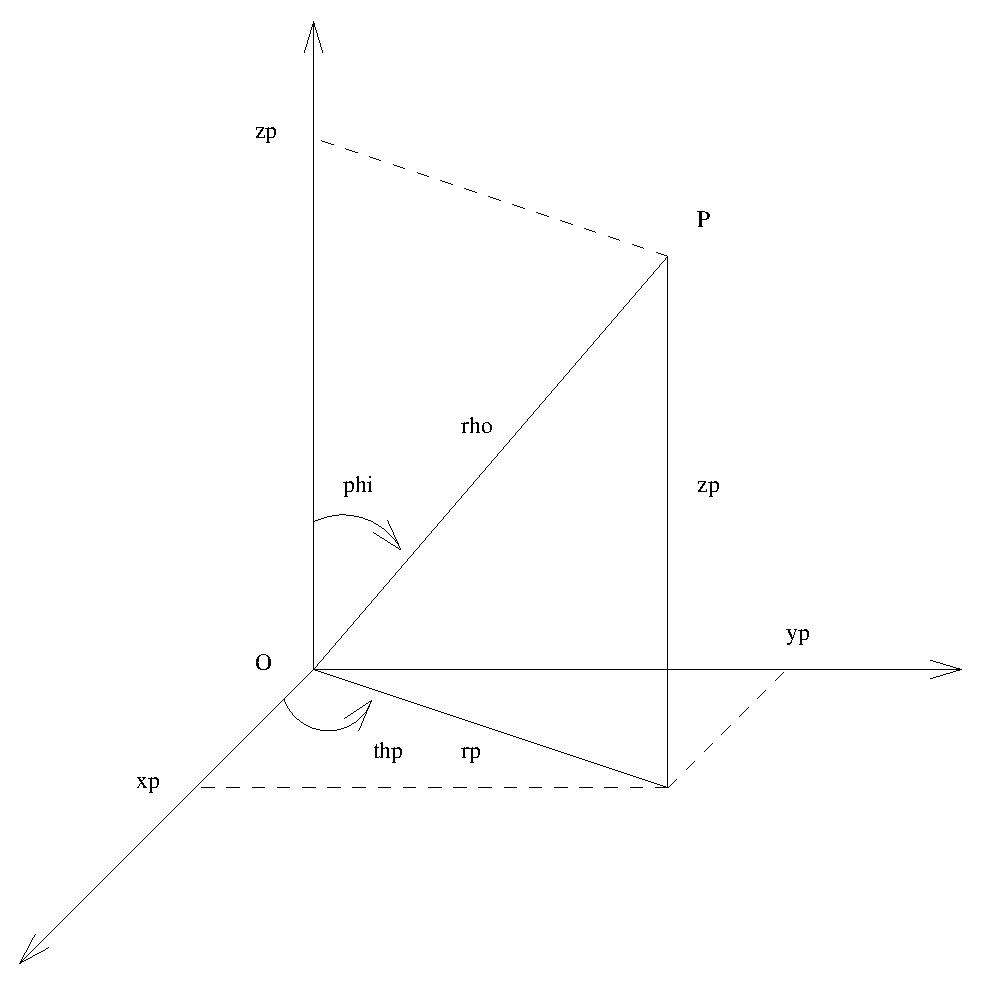
\includegraphics[height=2in]{../../modules/coordinate-systems/pictures/ok-cylindrical-spherical.eps}
\column{0.45\textwidth}
	\begin{itemize}
\item In Cartesian coordinates, a point $P$ is given by triple $(x_P, y_P, z_P)$.
\item<2-> We introduce alternative spherical coordinates $(\rho_P, \phi_P,\theta_P)$.
\begin{itemize}
\item \alert<3>{$\rho_P$: distance $|OP|$;}
\item \alert<4>{$\phi_P$: angle $Oz$ to $OP$;}
\item \alert<5>{$\theta_P$: angle $Ox$ to $OP_{xy}$.}
\end{itemize}
\item<6-> Coordinates range:
\begin{itemize}
\item \alert<7,8>{$\rho$:} \uncover<8->{\alert<8>{ $[0,\infty)$;}}
\item \alert<9,10>{$\phi$:}  \uncover<10->{\alert<10>{$[0, \pi]$;}}
\item \alert<11,12>{$\theta$:}  \uncover<12->{ \alert<12>{$[0,2\pi)$.}}
\end{itemize}
\end{itemize}
\end{columns}
\end{frame}
%\begin{frame}
\frametitle{Spherical curvilinear ``boxes''}


\begin{columns}
\column{0.4\textwidth}

\psset{xunit=1.5cm, yunit=1.5cm}
\begin{pspicture}(-2, -2)(2,2)
\tiny
\renewcommand{\fcScreen}{[-5 1 -2.4] 0}
\pstVerb{10 dict begin%
/rhoMin 1 def%
/rhoMax 2 def%
/thetaMin 20 def%
/thetaMax 70 def%
/phiMin 20 def%
/phiMax 70 def%
/xSph {theta cos phi sin rho mul mul} def%
/ySph {theta sin phi sin rho mul mul} def%
/zSph {phi cos rho mul} def%
}%
\fcAxesIIId{2}{2}{2}
\uncover<10->{
\pscustom*[linecolor=pink]{%
\fcCurveIIId{phiMin}{phiMax}{ 3 dict begin /rho rhoMin def /phi t def /theta thetaMin def xSph ySph zSph end}
\fcCurveIIId{rhoMin}{rhoMax}{ 3 dict begin /rho t def /phi phiMax def /theta thetaMin def xSph ySph zSph end}
\fcCurveIIId{thetaMin}{thetaMax}{ 3 dict begin /rho rhoMax def /phi phiMax def /theta t def xSph ySph zSph end}
\fcCurveIIId{phiMax}{phiMin}{ 3 dict begin /rho rhoMax def /phi t def /theta thetaMax def xSph ySph zSph end}
\fcCurveIIId{thetaMax}{thetaMin}{ 3 dict begin /rho rhoMax def /phi phiMin def /theta t def xSph ySph zSph end}
\fcCurveIIId{rhoMax}{rhoMin}{ 3 dict begin /rho t def /phi phiMin def /theta thetaMin def xSph ySph zSph end}
}%
}%
\fcLineIIId[linestyle=dashed]{[0 0 0]}{[0 2 0]}

\uncover<7->{\fcCurveIIId{rhoMin}{rhoMax}{ 3 dict begin /rho t def /phi phiMin def /theta thetaMin def xSph ySph zSph end}}
\uncover<5->{\fcCurveIIId{rhoMin}{rhoMax}{ 3 dict begin /rho t def /phi phiMax def /theta thetaMin def xSph ySph zSph end}}
\uncover<9->{\fcCurveIIId[linestyle=dashed, linecolor=red]{rhoMin}{rhoMax}{ 3 dict begin /rho t def /phi phiMin def /theta thetaMax def xSph ySph zSph end}}
\uncover<9->{\fcCurveIIId[linestyle=dashed, linecolor=red]{rhoMin}{rhoMax}{ 3 dict begin /rho t def /phi phiMax def /theta thetaMax def xSph ySph zSph end}}

\uncover<8->{%
\fcCurveIIId[linestyle=dashed, dash = 2.6pt,  linecolor=red] {thetaMin}{thetaMax}{ 3 dict begin /rho rhoMin def /phi phiMin def /theta t def xSph ySph zSph end}
\fcCurveIIId{thetaMin}{thetaMax}{ 3 dict begin /rho rhoMax def /phi phiMin def /theta t def xSph ySph zSph end}
\fcCurveIIId[linestyle=dashed, linecolor=red]{thetaMin}{thetaMax}{ 3 dict begin /rho rhoMin def /phi phiMax def /theta t def xSph ySph zSph end}
\fcCurveIIId{thetaMin}{thetaMax}{ 3 dict begin /rho rhoMax def /phi phiMax def /theta t def xSph ySph zSph end}
}%

\uncover<4->{\fcCurveIIId{phiMin}{phiMax}{ 3 dict begin /rho rhoMin def /phi t def /theta thetaMin def xSph ySph zSph end}}
\uncover<9->{\fcCurveIIId[linestyle=dashed, linecolor=red]{phiMin}{phiMax}{ 3 dict begin /rho rhoMin def /phi t def /theta thetaMax def xSph ySph zSph end}}
\uncover<6->{\fcCurveIIId{phiMin}{phiMax}{ 3 dict begin /rho rhoMax def /phi t def /theta thetaMin def xSph ySph zSph end}}
\uncover<9->{\fcCurveIIId{phiMin}{phiMax}{ 3 dict begin /rho rhoMax def /phi t def /theta thetaMax def xSph ySph zSph end}}
\pstVerb{end}
\end{pspicture}

\psset{xunit=1cm, yunit=1cm}
\begin{pspicture}(-2, -2)(2,2)
\tiny
\pstVerb{10 dict begin%
/rhoMin 1 def%
/rhoMax 2 def%
/thetaMin 20 57.2957795 div def%
/thetaMax 70 57.2957795 div  def%
/phiMin 20 57.2957795 div def%
/phiMax 70 57.2957795 div def%
}%
\fcAxesIIId[arrows=->, xLabel=$~~\rho$, yLabel=$~~\phi$, zLabel=$~~\theta$]{2.5}{3.8}{2.5}
\pscustom*[linecolor=cyan]{%
\fcPolyLineIIId{[rhoMin phiMin thetaMin] [rhoMax phiMin thetaMin] [rhoMax phiMax thetaMin] [rhoMax phiMax thetaMax] [rhoMin phiMax thetaMax] [rhoMin phiMin thetaMax] [rhoMin phiMin thetaMin]}
}
\fcLineIIId[linestyle=dashed]{[0 0 0]}{[0 3.8 0]}
\fcDotIIId{[rhoMin 0 0 ]}
\fcPutIIId[t]{[rhoMin 0 -0.2 ]}{$\rho_{min}$}
\fcDotIIId{[rhoMax 0 0 ]}
\fcPutIIId[t]{[rhoMax 0 -0.2 ]}{$\rho_{max}$}
\fcDotIIId{[0 0 thetaMin  ]}
\fcPutIIId[r]{[0 0 thetaMin]}{$\theta_{min}~~$}
\fcDotIIId{[0 0 thetaMax]}
\fcPutIIId[r]{[0 0 thetaMax]}{$\theta_{max}~~$}
\fcDotIIId{[0  phiMin 0  ]}
\fcPutIIId[b]{[0 phiMin 0.2 ]}{$~\phi_{min}$}
\fcDotIIId{[0  phiMax 0  ]}
\fcPutIIId[b]{[0 phiMax 0.2 ]}{$\phi_{max}$}

\fcLineIIId[linecolor=blue, linestyle=dashed]{[rhoMin phiMax thetaMin]}{[rhoMax phiMax thetaMin]}
\uncover<5-9>{\fcLineIIId[linecolor=red, linewidth=2pt, linestyle=dashed]{[rhoMin phiMax thetaMin]}{[rhoMax phiMax thetaMin]}}
\fcLineIIId[linecolor=blue]{[rhoMax phiMax thetaMin]}{[rhoMax phiMin thetaMin]}
\uncover<6-9>{\fcLineIIId[linecolor=red, linewidth=2pt]{[rhoMax phiMax thetaMin]}{[rhoMax phiMin thetaMin]}
}
\fcLineIIId[linecolor=blue]{[rhoMax phiMin thetaMin]}{[rhoMin phiMin thetaMin]}
\uncover<7-9>{\fcLineIIId[linecolor=red, linewidth=2pt]{[rhoMax phiMin thetaMin]}{[rhoMin phiMin thetaMin]}}
\fcLineIIId[linecolor=blue, linestyle=dashed]{[rhoMin phiMin thetaMin]}{[rhoMin phiMax thetaMin]}
\uncover<4-9>{\fcLineIIId[linecolor=red, linewidth=2pt, linestyle=dashed]{[rhoMin phiMin thetaMin]}{[rhoMin phiMax thetaMin]}}

\fcLineIIId[linecolor=blue, linestyle=dashed]{[rhoMin phiMax thetaMax]}{[rhoMin phiMax thetaMin]}
\fcLineIIId[linecolor=blue]{[rhoMax phiMax thetaMax]}{[rhoMax phiMax thetaMin]}
\fcLineIIId[linecolor=blue]{[rhoMax phiMin thetaMax]}{[rhoMax phiMin thetaMin]}
\fcLineIIId[linecolor=blue]{[rhoMin phiMin thetaMax]}{[rhoMin phiMin thetaMin]}
\uncover<8-9>{%
\fcLineIIId[linecolor=red, linestyle=dashed, linewidth=2pt]{[rhoMin phiMax thetaMax]}{[rhoMin phiMax thetaMin]}
\fcLineIIId[linecolor=red, linewidth=2pt]{[rhoMax phiMax thetaMax]}{[rhoMax phiMax thetaMin]}
\fcLineIIId[linecolor=red, linewidth=2pt]{[rhoMax phiMin thetaMax]}{[rhoMax phiMin thetaMin]}
\fcLineIIId[linecolor=red, linewidth=2pt]{[rhoMin phiMin thetaMax]}{[rhoMin phiMin thetaMin]}
}%
\fcLineIIId[linecolor=blue]{[rhoMin phiMax thetaMax]}{[rhoMax phiMax thetaMax]}
\fcLineIIId[linecolor=blue]{[rhoMax phiMax thetaMax]}{[rhoMax phiMin thetaMax]}
\fcLineIIId[linecolor=blue]{[rhoMax phiMin thetaMax]}{[rhoMin phiMin thetaMax]}
\fcLineIIId[linecolor=blue]{[rhoMin phiMin thetaMax]}{[rhoMin phiMax thetaMax]}
\uncover<9>{%
\fcLineIIId[linecolor=red, linewidth=2pt]{[rhoMin phiMax thetaMax]}{[rhoMax phiMax thetaMax]}
\fcLineIIId[linecolor=red, linewidth=2pt]{[rhoMax phiMax thetaMax]}{[rhoMax phiMin thetaMax]}
\fcLineIIId[linecolor=red, linewidth=2pt]{[rhoMax phiMin thetaMax]}{[rhoMin phiMin thetaMax]}
\fcLineIIId[linecolor=red, linewidth=2pt]{[rhoMin phiMin thetaMax]}{[rhoMin phiMax thetaMax]}
}%
\pstVerb{end}
\end{pspicture}

\column{0.6\textwidth}
\begin{itemize}
\item Cut off a rectangular box $B$ in the $\rho, \phi, \theta$-coordinates. 
$
B:=\left\{(\rho, \phi, \theta) |\left| \begin{array}{ccccc} 
\rho_{min} &\leq& \rho &\leq& \rho_{max} \\
\phi_{min} &\leq& \phi &\leq& \phi_{max}\\
\theta_{min} &\leq& \theta &\leq& \theta_{max}\\
\end{array}\right.\right\}
$
\item<2-> As $(\rho, \phi, \theta)$ traverse $B$, the point $P(\rho, \phi,\theta)$ traverses curvilinear ``box'' $Y$: %in the $x,y,z$-coordinates: 
\[
Y = \left\{ P(\rho, \phi, \theta) | (\rho, \phi, \theta)\in B \right\}.
\]
\item<3-> \alert<3-10>{ What is the shape of that curvilinear box?}
\item<11-> What is the volume?
\end{itemize}
\end{columns}
\end{frame}
}
\end{document}
